\section{Úvod}

Tato bakalářská práce se bude zabývat tvorbou aplikace pro tvorbu a zobrazování vstupních stránek osob, firem a jiných
institucí.
Takových aplikací existuje mnoho, nicméně žádná nekombinuje širší možnost i sdílení různých informací.
Proto jsem se rozhodl navrhnout a implementovat vlastní verzi v podobě responzivní webové aplikace, která bude
kombinovat různé typy údajů s vyhledáváním.

Jednostránkové vstupní stránky jsou moderní cestou jak sdílet všechny své veřejné kontaktní a jiné údaje se
svými zákazníky nebo sledovately.
Představují jakosi digitální rozšířenou alternativu k bežných fyzickým vizitkám, které však postrádají interaktivnost
spoustu důležitých údajů.

Dále se práce zaměří na analýzu implementačních technologií, hlavně pak na programovací jazyky a frameworky urychlující vývoj.
Technologií v dnešní době existuje celá řada a každým dnem přibývají nové.
Pro účely této práce se technologie rozdělí na front-endové a back-endové.
Front-endové budou pomáhat tvořit responzivní a interaktivní uživatelské prostředí pro koncové uživatele.
Back-endové na proti tomu budou tvořit konkrétní logiku aplikace na pozadí.
To zahrnuje operace jako manipulaci s uživatelskými daty nebo jejich agregaci.
Součástí této práce bude průzkum celosvětově využívaných technologií pro vývoj webových aplikací.
V případě front-endu se bude jednat o nějaký z Javascriptových frameworků: Vue, React, Swelte nebo Angular.
V rámci back-endu se práce zaměří na programovací jazyky Java, Javascript, C\#, PHP a další a také na
podpůrné nástroje v podobě databázových systémů.

Po zvolení vhodných technologií bude následovat navržení uživatelského prostředí společně s interním
datovým modelem a strukturou aplikace.
Tento návrh bude vzápětí implementován a jednotlivé části jeho postupu popsány.

Konečným krokem bude spuštění aplikace v produkčním prostředí přístupné veřejnosti s potřebnými zabezpečeními.

\section{Cíl práce}

V první řadě bude nezbytné zjistit jaké informace bude vhodné umožňovat uživatelům zobrazovat na jejich
vstupních stránkách a jak s těmito informacemi nakládat napříč aplikací.
Dále bude následovat analýza a provonání programovacích jazyků a frameworků společně s jejich výhodami a nevýhodami.
Výsledný výběr bude kombinací požadavků aplikace a výhod jednotlivých technologií.

Implementace pak bude vycházet z návrhu datového modelu a struktury aplikace.
U jednotlivých řešených problémů bude problém popsán, navrženy možné postupy a samotná výsledná implementace.

Primárním cílem je vytvořit funkční interaktivní webovou aplikaci umožňující intuitivně svým uživatelům
tvořit, spravovat a sdílet své vstupní stránky mezi jinými uživateli.
Aplikace by měla také podporovat všechny využívané rozměry zařízení, aby byl zaručen přístup k aplikaci z mobilních
i desktopových zařízení s minimálním omezením pro uživatele.
Rovněž by aplikace měla být jednoduše spustitelná a udržitelně provozována v produkčním prostředí.

\section{Vstupní stránky pro osoby a instituce}

Vstupní stránky pro osoby a instituce jsou prezentační jednostránkové webové stránky.
Tyto stránky slouží k představení daného subjektu/objektu koncovému uživateli, který hledá základní
informace o daném subjektu.
Kromě základních informací většinou obsahují všemožné kontaktní údaje a odkazy na sociální sítě pro
získání mnohem detailnějších informací.
Některé stránky umožňují reprezentovat i například firemní strukturu nebo lokaci.

Možnosti informací, které lze definovat na takových stránkách nejsou jasně definované, spíše jsou
určeny aplikací poskytující tyto služby.
Kvůli tomu každá již existující aplikace zpřístupňuje jiné informace autorům jiným stylem.

Tento typ stránek je velice vhodný pro sdílení svých osobních údajů a funguje jako takový rejstřík uživatelových
informací.
Vstupní stránky by se dalo popsat jako digitální rozšířené vizitky nejen pro firmy.

Pro tvorbu takovýchto stránek existuje nepřeberné množství webových aplikací, kde lze
tyto prezentace jednoduše tvořit.
Ne všechny ale nabízí všechny zmíněné možnosti a je tak na autorovi, jakou webovou aplikaci zvolí.

\section{Existující aplikace}

Existuje spousta webových aplikací, které by se dali považovat za řešení popsané problematiky
Nicméně žádná momentálně nekombinuje prvky sdílení kontaktních údajů, sociálních sítí a firemní struktury s plně
fulltextovým vyhledáváním bez nutnosti registrace nebo rušení sociálními prvky jako jsou zprávy nebo feedy novinek
náhodných osob a firem, případně ukládání subjektů do oblíbených s možností kategorizace či poznámek nebo globálnosti
platformy.
U většiny takových aplikací se totiž spoléhá na navigaci na cílené subjekty pomocí přímých odkazů, které si daný subjekt
vloží na své sociální sítě nebo vizitky.

Zde byly popsány současné nejznámější existující aplikace pro porovnání s později navrhovaným a implementovaným řešením.

	\subsection{Linktree}

	Pravděpodobně nejrozšířenější takovou aplikací v zahraníčí je Linktree.
	Ta se zabývá především zobrazováním odkazů na sociální sítě a rozsáhlím přízpůsobením.
	Momentálně však neumožňuje fulltextově ani jinak vyhledávat jednotlivé uživatele nebo ukládat ostatní uživatele
	do oblíbených.
	Není ani jistota, že jednotlivé odkazy směřuje opravdu na skutečně sociální sítě, protože uživatelé si mohou ke každému
	odkazu zvolit vlastní ikony.
	Nezabývá se ani firemní hierarchií nebo otevírací dobou.
	Na druhou stranu, poskytuje spoustu napojení na externí aplikace, především pak ty statistické nebo e-commercové.

	\subsection{LinkedIn}

	Další významou aplikací je LinkedIn.
	Ta však směřuje své zaměření spíše na firemní prostředí a pracovní zkušenosti uživatelů.
	Informace navíc nejsou veřejně dostupné bez registrace.
	Oproti Linktree ale obsahuje fulltextové vyhledávání.
	Nevýhodou můžou být sociální prvky aplikace generující nevyžádané spojení s cizími uživateli a firmami nebo
	reklami ostatních firem.
	I přesto že se zaměřuje na firmy, není snadné dohledat firemní struktury nebo otevírací dobu.


	\subsection{AllMyLinks}

	Méně známou alternativou je služba AllMyLinks.
	Ta nabízí velice podobné funkce jako Linktree.
	Také nabízí pouze sdílení odkazů na sociální sítě.
	Stejně jako Linktree neposkytuje pokročilou podporu o ověřování odkazů oproti sociálním sítím, což má za následek
	nevěryhodnot odkazů a ošklivé uživatelské ikony.

	\subsection{Swopi}

	Swopi je další alternativou Linktree.
	Navíc se ale zabývá výrobou a prodejem chytrých fyzických karet a štítků pro rychlé zobrazení uživatelského profilu.
	Software je ale značně neintuitivní a neposkytuje více odkazů na jednu sociální síť.

	\subsection{Firmy.cz}

	Mezi české nepřímé alternativy by se dali zařadit i Firmy.cz, která se ale podobně jako LinkedIn zabývají
	spíše firmami a jejich zobrazení na mapě.
	Nabízí vyhledávání, otevírací dobu a základní kontakty, externí odkazy a firemní struktura jsou však značně omezené.
	Služba je navíc cílená pouze na české publikum.

	\subsection{Zlaté stránky}

	Obdobou Firmy.cz trpící podobnými problémy je další česká služby Zlaté stránky

\section{Návrh vlastní aplikace}

Implementovaná aplikace bude oproti konkurenčních řešení kombinovat více různých typů informací, aby tak pokryla
většinu požadavků jak soukromých osob, tak firem nebo objektů.
Základní obecnou jednotkou reprezentující takový subjekt či objekt bude karta; odvozenina z anglického překladu vizitky "business card".
Každá karta tak bude jakousi digitální pokročilou náhradou klasických vizitek nevztahující se pouze na osoby a jejich
hlavní kontaktní údaje.
Cílem je umožňovat vyhledávat a sdílet informace kromě soukromých osob a firem i události, produkty, místa, umělecká díla a mnohem více.
Jedinou podmínkou pro takový subjekt nebo objekt je existence alespoň jednoho údaje důležitého pro ostatní osoby.
Tím může být kontaktní údaj, odkaz na jiné webové stránky (např.: sociální sítě), geografická pozice nebo
nějaká hierarchie ostatních subjektů či objektů.

	\subsection{Oblíbené karty}

	Ostatní uživatelé pak budou mít možnost takové karty, které je nějakým způsobem zajímají, uložit do svého profilu pro
	zjednodušení zpětného dohledání například kontaktních údajů.
	Kromě obyčejného uchování oblíbených karet bude možné takové karty seskupovat do vlastních upravitelných složek pro
	lepší organizaci a komentovat vlastními soukromými poznámkami.
	Tyto funkce umožní uživatelům komunikujícím s velkým počtem subjektů vyznat se v kontaktních údajích a poznámkách
	například s poslední komunikace nebo podrobností o daném subjektu bez nutnosti ručně takové informace spravovat v
	textových editorech nebo papírových poznámkách.

	\subsection{Viditelnost karet}

	Protože vyplnění takové karty může být zdlouhavý proces, i za předpokladu intuitivního \ac{UI}, je potřeba umožnit
	uživatelům karty skrýt do té doby, než budou připravené ke zveřejnění.
	Zároveň ale takovou rozpracovanou kartu může uživatel chtít někomu vzdáleně ukázat například pro ověření správnosti informací
	bez zveřejňování.
	Karty tak budou moct mít dvě viditelnosti: veřejná a skrytá.
	Veřejná karta bude mít jednoduchou zapamatovatelnou \ac{URL} adresu a bude ji možné vyhledávat pomocí fulltextového vyhledávače.
	Skrytá karta nebude vyhledatelná pomocí vyhledávače, nicméně uživatelé vlastnící \ac{URL} odkaz na danou kartu budou mít přístup
	ke zobrazení dané karty.
	Skrytá karta bude mít navíc možnost vygenerování náhodné \ac{URL} pro znemožnění uhádnutí \ac{URL} adresy nepovolenou osobou.

	\subsection{Karetní informace}

	Každá karta, jak již bylo nastíněno, bude mít možnost zobrazovat různé informace pro uživatele.
	Definovatelné informace budou vždy dané, tj. budou mít vlastní strukturu v kódu, validaci správnosti hodnot a specializované
	\ac{UI}.
	Nebude možné uživatelem definovat náhodné informace, aby se předešlo ke zhoršení čitelnosti informací karet.
	Toto rozhodnutí by mělo pomoci především uživatelům nepříliš zdatných v dodržení přehlednosti většího množství
	informací za pomoci předem daného formátu zobrazení daných informací.
	Je však potřeba strukturu navrhnout dostatečně univerzálně, aby bylo možné v budoucnu implementovat další typy informací
	definovatelných na kartách.
	Momentálně podporovanými takovými informacemi budou:
	\begin{itemize}
		\item fotografie/avatar
		\item kategorizační štítky
		\item popisek
		\item základní kontaktní údaje
		\item odkazy na profily na sociálních sítí
		\item generické odkazy na jakékoliv externí webové stránky
		\item geografická lokace
		\item hlavní otevírací doba
		\item kanceláře, pobočky
	\end{itemize}

	Pro rychlé vizuální rozpoznaní karty bude mít autor k dispozici možnost nahrát vlastní fotografii nebo avatar s logem.
	Fotografie nebo avatar dokáže dostatečně odlišit jednotlivé karty bez nutnosti čtení názvu nebo popisku ke zjistění o
	jakou kartu se vlastně jedná.

	Kategorizační štítky budou sloužit pro globální kategorizaci karet pro úvodní povědomí uživatele o jakou kartu se jedná
	a hlavně pro vyhledání karet ve stejné kategorii.
	To se může hodit pro seskupení například osob s určitým povolání nebo vyznávaným životním stylem.
	Konkrétní využití je však na konkrétních uživatelích.
	Štítku uživatel bude moct definovat několik nebo žádný.

	Popisek bude sloužit především pro stručnou definici obsahu karty, tj. co daná karta reprezentuje.
	Předpokládá se tedy, že popisek karty bude zodpovídat některé z následujících otázek?
	\begin{itemize}
		\item Je to osoba, firma, událost, dílo nebo předmět?
		\item Čím daný subjekt či objekt zabývá v profesní nebo soukromé sféře?
		\item Proč je daný subjekt či objekt zajímavý?
	\end{itemize}
	Popisek bude mít omezenou velikost a nebude povinný, nicméně silně doporučovaný.

	Základními kontaktními údaji se v případě těchto karet rozumí: telefonní číslo, hlavní emailová adresa, hlavní
	webové stránky a identifikační číslo (\noindent\ac{IČO}).
	Uživatel si pak vybere jaké z těchto údajů bude chtít zveřejnit a jaké nikoliv.

	Pro většiny karet, zejména pak pro karty reprezentující soukromé osoby, budou nejdůležitější odkazy na sociální sítě.
	Pro jednoduché rozlišení mezi jednotlivými sítěmi a poskytnutí koncovým uživatelům jistotu, že daný odkaz skutečně
	směřuje na ověřenou doménu dané sociální sítě, systém bude mít předefinované podporované sociální sítě.
	Každá taková definice bude jakousi šablonou pro výsledné odkazy na sociální sítě a bude obsahovat oficiální název,
	názvy podle kterým bude možné sít vyhledat, ikonu, šablony validních \ac{URL} adres a kategorii.
	Uživatel pak bude moct při tvorbě karty vybrat konkrétní síť ručně ze seznamu nebo nechat aplikaci nalézt správnou
	síť podle vložené \ac{URL} adresy.
	Šablony sítí budou kategorizované a bude možné je vyhledávat podle názvu pro jednodušší dohledání.
	Po vložení konkrétní \ac{URL} adresy vznikne konkrétní odkaz držící informaci o použité šabloně, cílové \ac{URL} adresy a
	popisku pro rozeznání různých odkazů na stejné sociální sítě.
	Díky definovaným šablonám reprezentující rozsah validních \ac{URL} pro konkrétní sociální síť bude aplikace schopna
	validovat konkrétní \ac{URL} adresy zda-li odpovídají alespoň jedné šabloně a jestli zadaná \ac{URL} adresa skutečně existuje.
	To jednak umožní autory karet upozornit na nesprávné \ac{URL} adresy a koncovým uživatelům karet poskytne zmiňovanou jistotu
	\ac{URL} adresy skutečně vedoucí na prezentovanou síť.

	Generické odkazy budou podobné odkazům na sociální sítě.
	Rozdíl však bude ve volnosti zadat jakoukoliv validní \ac{URL} adresu.
	Taková adresa sice bude stále validovaná aplikaci pro existenci, nebude už však validovaná proti žádnému rozsahu
	\ac{URL} adres.
	To umožní autorovi karty odkazovat na jakékoliv webové stránky, ale znemožní poskytnutí jistoty pravosti odkazu
	pro koncové uživatele.
	Bohužel není možné jednoduše strojově zjistit jestli odkaz nevede na podvodnou stránku.
	Takové stránky jsou obtížné rozeznat od originálních webových stránek i pro pravidelné uživatelé originálních stránek.
	Navíc podvodné stránky každým dnem přibývají a autoři takových webů jsou stále sofistikovanější.

	Důležitou informací pro firmy, události, pobočky atd. je geografiká lokace sídla.
	Ta umožní koncovým uživatelům nalézt subjekt či objekt, reprezentovaný kartou, v reálném světě.
	Zároveň poskytne možnost zobrazit karty v blízkém okolí daného uživatele pomocí mapy.
	Uživatel tak jednoduše zjistí jaké firmy, osoby nebo události se nachází v okolí jeho bydliště, zaměstnaní nebo
	cílové destinace.

	Firmy a obchody většinou mají nějakou provozní/otevírací dobu, kdy jsou zaměstnanci schopni obsloužit své zákazníky.
	Tato informace je navíc uživateli vyhledávaná opakovaně a je tedy nutné, aby byla po ruce a zobrazovala všechny potřebné
	informace.
	Každá karta tak bude moct definovat otevírací dobu každého dne v týdnu s volitelnou přestávkou.
	Uživatelé tak kromě definovaných otevíracích dob uvidí i informaci o tom, jaká otevírací doba pro daný den platí
	a za jak dlouho daný subjekt bude mít otevřeno, popřípadě kolik času zbývá do konce otevírací doby.

	Nedílnou součástí větších firem a institucí jsou pobočky a kanceláře rozmístěné v různých koutech světa.
	Každá taková pobočka má své zaměstnance, geografickou lokaci a v některých případech i vlastní otevírací dobu.
	Autor karty tak může definovat své pobočky či kanceláře a volitelně je obohatit o zmíněné rozšiřující informace.
	Každá taková pobočka může mít vlastní otevírací dobu, i přes to, že samotná karta může mít již hlavní otevírací dobu
	definovanou, nebo nemusí mít žádnou.
	Pro klienty je pak vhodné mít definovanou i lokaci dané pobočky.
	Podstatnou částí bude možnost přiřadit zaměstnance nacházející se v dané pobočce pro snadné kontaktování přímo konkrétních
	osob.
	Zaměstnanec bude mít definovanou pracovní pozici a jméno, volitelně pak ještě fotografii a základní kontaktní údaje
	v podobě emailové adresy telefonního čísla.
	Každý takový zaměstnanec bude reprezentován speciálním typem karty pro možnost uložení konkrétních zaměstnanců mezi oblíbené
	karty.

	\subsection{Typy karet}

	Aby bylo možné definovat pro karty různého zaměření jiné podporované informace, bude existovat podpora pro typy karet.
	Každý typ bude definovat účel karty, možné informace a platné použití.
	Koncoví uživatelé budou schopni díky této univerzalitě ukládat karty mezi oblíbené bez rozdílů.
	Momentálně dostupnými typy budou: obecná karta a karta zaměstnance.
	Obecná karta bude umožňovat specifikovat všechny výše zmíněné informace a každý uživatel ji bude moct přímo vytvořit.
	Karta zaměstnance bude automaticky nepřímo tvořena při tvorbě zaměstnanců poboček.
	To umožní pro zobrazit detail jednotlivých zaměstnanců, mít unikátní odkaz na každého zaměstnance nebo vyhledávat
	přímo karty zaměstnanců s referencí na rodičovskou firmu.
	Typy karet se ale mohou v budoucnu rozrůst o další specializované typy, a je proto nutné s takovým rozšířením při
	implementaci počítat.

	\subsection{Vyhledávání karet}

	Velmi podstatnou součástí výsledné aplikace je schopnost vyhledávat a objevovat karty podle požadavků koncového uživatele.
	Pro zajištění těchto funkcí bude aplikace umět fulltextově vyhledávat a geograficky zobrazovat karty na mapě světa.
	Díky fulltextovému vyhledávání bude uživatel schopen vyhledávat chtěné karty podle frází obsažených v názvu,
	popisku, kontaktních údajích, odkazech, názvů poboček a karet zaměstnanců.
	Výsledky takového vyhledávání budou seřazený podle relevantnosti vzhledem k hledané frázi.
	Mimo konkrétního vyhledávání uživateli bude zobrazena mapa světa se zaměřením na jeho současnou lokaci zobrazující
	karty a pobočky jako body v mapě.
	Každý bod bude obsahovat souhrn nejdůležitějších informací z reprezentující karty nebo pobočky.
	Takovou informací může být název, štítky, otevírací doba konkrétního dne, odkazy nebo zaměstnanci.
	Díky těmto funkcím budou uživatelé schopni objevovat nové subjekty a objekty bez nutnosti znalosti \ac{URL} adres
	konkrétních karet.

	\subsection{Dostupnost aplikace}

	Cílem aplikace je poskytnout globálně komukoliv bez omezení přístup k veřejným informacím.
	Na rozdíl od některé konkurence nebude vyžadováno po uživatelích registrace ve výsledné aplikaci pro přístup k vyhledávání
	nebo samotným kartám a jejich informacím.
	Jedinou opodstatněnou výjimkou pro nutnost registrace by se v budoucnu mohli stát karty s příznakem 18+.
	Registrovaný účet uživatele by pak sloužil pro ověření věku daného uživatele podle data narození.
	Tento požadavek však současné verzi navrhované aplikace není řešen.
	Dalším požadavkem je umožnit přístup k informacím z jakékoliv země světa.
	Budoucím cílem je postupně lokalizovat aplikaci do dalších jazyků pro ještě větší dostupnost v zemích mluvících
	jiným než anglickým jazykem.
	Nicméně chybějící jazyk dané země nesmí být sám o sobě důvod pro nedostupnost aplikace v dané zemi, uživatelé by
	měli být vždy schopni používat minimálně výchozí anglickou lokalizaci.

	\subsection{Uživatelské účty}

	Jak již bylo v předchozí kapitole nastíněno, uživatelské účty budou volitelnou funkcí aplikace přinášející výhody
	nemožné implementovat bez existující účtu.
	Mezi takové výhody bude z počátku patřit tvoření karet a ukládání cizích karet mezi oblíbené.
	Tyto funkce vyžadují uživatelský účet, aby bylo možné určit kdo má právo upravovat a mazat dané vytvořené karty
	a ukládat soukromé data uživatele jako jsou oblíbené karty a jejich poznámky bez viditelnosti ostatním uživatelům.
	Uživatelské účtu jsou tak tedy spíše bezpečnostním nástrojem pro správu dat v tvořené webové aplikaci, nikoliv
	nástrojem pro získání dat uživatelů pro například pro zpracování nesouvisející se záměrem aplikace nebo prodej dat
	společnostem zabývajících se inzercí reklamy.
	Uživatelské účty jako takové nebudou reprezentovat vždy jen jednu kartu.
	Místo toho každý účet bude moct vytvořit několik karet a účet bude představovat jen vlastníka neviditelného pro
	veřejnost.
	To umožní uživatelům s potřebou více karet pro různé subjekty či objekty používat jeden registrovaný účet místo
	separátního pro každou kartu jako tomu bývá zvykem u konkurence.

	Kromě těchto hlavních funkcí uživatelských účtů, správná aplikace musí svým zaregistrovaným uživatelům poskytnout
	i nástroje pro správu účtů jako takových.
	Každý uživatelský účet bude identifikován jednoznačně pouze podle emailové adresy.
	Aplikace nebude vyžadovat žádné další údaje v podobě jména, bydliště a podobně, protože pro tyto nejsou potřeba pro
	provoz aplikace a aplikace nebude zpracovávat uživatelská data jiným způsobem.
	Emailová adresa místo uživatelského jména byla zvolena z důvodu možnosti informovat uživatele o různých událostech
	v aplikaci bez nutnosti otevírat samotnou webovou aplikaci.
	Takové události mohou zahrnovat potvrzení změny emailové adresy, upozornění na změnu hesla nebo třeba vyžádání obnovy
	zapomenutého hesla.
	Mimo samotné registrace a přihlášení, aplikace bude umožňovat změnu emailu bezpečně obnovit zapomenuté heslo, kompletně
	smazat vytvořený účet se všemi jeho daty nebo odhlásit uživatele ze všech přihlášených zařízení.
	Přihlášení pomocí emailové adresy a hesla bude navíc rozšířeno o přihlášení a registraci skrze účty třetích stran.
	To zjednoduší a hlavně zrychlí registraci a přihlášení uživatelů využívající služby Googlu, Facebooku nebo třeba
	GitHubu, kde již daní uživatelé můžou být zaregistrovaní.
	Při registraci v aplikaci pomocí některého z poskytovatelů pak poskytovatel předá aplikaci základní údaje automaticky
	a uživatel pouze registraci potvrdí bez nutnosti cokoliv ručně vyplňovat.

		\subsubsection{Prémiové funkce}

		Aby bylo možné obecně jakoukoliv webovou aplikaci dlouhodobě provozovat, je nutné zajistit financování provozu
		produkčního prostředí.
		Možností je velké množství a záleží na představivosti vlastníka aplikace.
		Nejčastějšími praktikami jsou: prodej produktů nebo služeb, zobrazování reklamy a placené plány s prémiovými funkcemi.
		V případě této aplikace by bylo možné nabízet a prodávat fyzické produkty v podobě například speciálních čipových karet
		konfigurovatelných pro přesměrování na uživatelem definovaných karet.
		Avšak prodej jakýchkoliv fyzických produktů není hlavním cílem této aplikace, zejména kvůli přidané zátěži
		pro provoz.
		Zobrazování reklam při navigování aplikací by bylo možné a nepřidalo by toto řešení nadbytečnou zátěž na provoz,
		nicméně uživatelské rozhraní by značně trpělo svojí razantně sníženou přehledností a nechtěným proklikům zobrazovaných
		reklam což by mohlo vést ještě k frustraci uživatelů.
		Existuje navíc značné procento uživatelů využívající speciální nástroje prohlížečů pro blokování všech reklam.
		Ideální variantou pro tento typ aplikace se jeví zavedení placených plánu s prémiovými funkcemi.
		Zaregistrovaný uživatel standardně bude mít bezplatný plán poskytující uživateli základní omezené funkce, ale
		bude moct si aktivovat prémiový placený plán odemykající všechny zbylé funkce co aplikace bude nabízet.
		Toto řešení zamezí zhoršení uživatelského rozhraní a celkově nebude omezovat běžné koncové uživatele.
		Zároveň řešení nebude ovlivněno nástroji pro blokování reklam a nebude narušovat soukromí uživatelů v podobě
		sbírání uživatelských dat z reklam.
		Nevýhodou o proti reklamám je přidaná náročnost implementace systému umožňující uživatelům přepínat a platit
		plány a hlavně zamezit uživatelům s bezplatným plánem využívat prémiové funkce.
		Avšak na rozdíl od fyzických produktů, kde přidaná zátěž je stálá, tato zátěž se týká především počátku implementace.
		Další možnou nevýhodou je málo uživatelů platící si prémiový plán, protože pokud nebude dostatečný počet
		platících zákazníků, nebude dostatečný příjem pro produkční provoz.

		Konkrétním řešením pro tuto webovou aplikaci bude zavést limity pro bezplatný plán a umožnit uživatelům jednoduše
		přejít na placený.
		Kromě samotných plateb bude možné uplatňovat kupóny, které aktivují prémiový plán na konečnou dobu a poté se plán
		automatické přepne zpět na bezplatný.
		Pokud uživatel budem mít na svém účtě aktivované prémiové funkce při vypršení prémiového plánu, bude nucen
		data zahrnující prémiové funkce odstranit jinak budou automaticky skryta.
		Samotné limity se budou týkat především karet.
		V případě bezplatného plánu bude mít uživatel k dispozici omezený počet karet, které může vytvořit.
		V rámci každé karty pak budou další omezení v podobě nemožnosti tvořit pobočky a zaměstnance.
		Důležité je připravit takový systém, aby bylo možné co nejjednodušeji limity upravovat a případně přidávat další
		s novými prémiovými funkcemi.

	\subsection{Bezpečnost}

	V dnešní době s přibývajícími podvodnými stránkami a sofistikovanějšími útočníky je čím dál více důležité myslet i
	na zabezpečení webových aplikací.
	Kromě základní již běžné praktiky hashování hesel bezpečným algoritmem je nutné zabezpečit mnohem více.
	V první řadě jde komunikaci mezi prohlížečem a serverem, aby nemohl útočník odposlouchávat posílaná data a následně
	se třeba vydávat za určitého uživatele.
	S kradením identity uživatelů souvisí i další praktiky jako CSRF nebo kradení session.
	Z pohledu samotného kódu aplikace je zas nutné připravit systém práv a taková práva uživatelů před vykonáním
	požadovaných akcí ověřovat, aby jeden uživatel nemohl upravovat data jiných uživatelů nebo jinak škodit.

	\subsection{UI}

	Aby byla aplikace schopna konkurovat rozsáhlé konkurenci, musí kromě své základní funkčnosti poskytovat i přehledné
	a vzhledné uživatelské prostředí (\noindent\ac{UI}).
	Navržené \ac{UI} by tak mělo uživateli zjednodušovat přístup k informacím a akcím, které chce provést bez nutnosti
	zdlouhavého hledání skrze aplikací.
	Kvůli velkému procentu využívání internetu na mobilních zařízení je žádoucí připravit prostředí automaticky se
	přizpůsobující velikosti zařízení při zachování přehlednosti a dostupnosti i na malých.
	Hlavním cílem je uživatelům mobilních zařízení poskytnou webovou aplikaci přibližující se svým rozvržením a pohodlím
	nativním aplikacím stejně jako tak jako pro uživatele osobních počítačů s velkými obrazovkami pomocí jedné
	aplikace díky dynamické přizpůsobitelnosti \ac{UI}.
	Tento koncept se navíc v budoucnosti dá dále rozšířit o skutečnou mobilní aplikaci díky některým technologiím
	bez nutnosti tvořit vlastní nativní aplikaci kopírující funkce webové aplikace což je velmi nákladné.

% ################################
\section{Technologie pro vývoj}

Vývoj jakékoliv aplikace od nuly až po provoz v produkčním prostředí zahrnuje spustu kroků a každý takový krok
lze pojmout několika způsoby.
Před samotným vývojem je tak potřeba důkladně promyslet a naplánovat jaké má projekt požadavky, co je cílem samotného projektu
a také jaký je rozpočet pro jeho vývoj.
Od těchto cílů se pak odvíjí způsob vývoje a především výběr technologií a nástrojů použitých při vývoji.
Ty spolu musí být dostatečně kompatibilní a tvořit efektivní celek.
Při výběru nevhodných technologií se totiž může stát, že v průběhu vývoje vývojáři narazí na problém, který je buď
s použitými technologiemi neřešitelný, protože daná technologie třeba nebyla navržena pro konkrétní úlohu, nebo
je nutné problém obejít a to může způsobit komplikace v budoucnu v podobě malé výkonnosti aplikace nebo příliš
složitého zdrojového kódu.
V dnešním moderním světě existuje spousta webových technologií, které umožňují a většinou i značně usnadňují vývoj
webových stránek, aplikací či mikroslužeb.
Avšak nové alternativní technologie přibývají každým dnem a může být mnohdy obtížné i pro zkušené
vývojáře se zorientovat a vybrat ty správné pro daný projekt.
Při rozhodování je důležité vybírat nejen podle popularity, ale především podle typu projektu, ten totiž může zásadně
ovlivnit, jaké technologie jsou vhodné a které nikoliv.

Kromě webových technologií použitých přímo pro vývoj aplikace je vhodné se při návrhu zabývat i technologiemi a nástroji
pro:
\begin{itemize}
	\item uchovávání uživatelských dat
	\item uchovávání souborů a poskytování jejich variant
	\item návrh uživatelského rozhraní
	\item komunikaci s uživateli jinými kanály než je samotná aplikace
	\item běh aplikace ve vývojovém a produkčním prostředí
\end{itemize}

Webové technologie se navíc primárně rozdělují na dvě kategorie: front-endové a back-endové.
Obě obsahují rozdílné technologie zejména kvůli tomu, že se každá z nich zabývá odlišnou částí
vývoje.
Existují ale i technologie spadající více či méně do obou kategorií, avšak v každé plní trochu jiný účel.
Nejrozšířenějším takovým kandidátem je \noindent\ac{JS} dominující v současné době oběma kategoriím.

	\subsection{Techonologie pro návrh UI a UX}

	Návrh \ac{UI} je jedním z nejdůležitějších kroků pro úspěšnou aplikaci.
	Společně s uživatelským zážitkem (\noindent\ac{UX}) z velké části rozhodují zda aplikace nebo webová prezentace
	uživatele zaujme a bude jí nadále používat nebo přejde ke konkurenci.
	Je důležité navrhnout moderní, přehledné a hlavně intuitivní \ac{UI} neobtěžující koncového uživatele svojí složitostí.
	Kromě na vizuálně přívětivého \ac{UI} je stěžejní myslet na \ac{UX}, kdy použité prvky jako tlačítka, nadpisy,
	vyskakovací okna musí být důkladně promyšleny, aby uživatele podvědomě naváděli uživatele k jeho cíli.
	U jednotlivých prvků jde tak především o tvary, barvy, stíny, rozestupy mezi prvky a textem nebo třeba kontrast prvků
	mezi sebou.
	Dobré je myslet i na uživatele s různými omezeními.
	Například pro úplnou slepotu je možné do webové stránky přidat speciální metadata umožňující prohlížečům správně
	předčítat obsah stránky.
	Pro barvoslepost je zas dobré myslet na správný kontrast vybrané barevné palety při použití s textem, aby byl
	čitelný pro všechny.
	Návrh \ac{UI} ještě před samotnou implementací může navíc zásadně šetřit čas vývojáře, protože v úvodních krocích
	se design často mění, a pokud by měl vývojář kromě každou úpravu ještě implementovat, zabralo by to dvojnásobek času.

	Pro návrh \ac{UI} a \ac{UX} před samotným začátkem vývoje nebo i pro dodatečné úpravy existují specializované
	grafické nástroje.
	Použít lze i tradiční grafické nástroje, ty ale nenabízí funkce pro vzájemnou kolaboraci mezi
	členy v týmu nebo přidávání interaktivních prvků přímo do grafického návrhu pro demonstraci fungování budoucí
	aplikace.
	Nejpopulárnějšími nástroji se staly Figma, Sketch a Adobe DX a z toho Figma a Adobe XD poskytují dokonce bezplatné
	varianty s určitými omezeními \cite{design_tools_database}.
	S pomocí nich je snadné navrhnout základní drátový model pro návrh struktury, grafický model pro vizualizaci
	vzhledu i interaktivní demo sestavené z předchozích modelů.
	Tyto modely pak značně usnadňují tvorbu \ac{UI}, protože vývojář tvořící výslednou stránku nemusí vymýšlet
	vzhled a strukturu stránku při samotném vývoji stránky.
	Místo toho se může zabývat čistou implementací až finální verze \ac{UI}.
	Samotný výběr konkrétního nástroje je otázkou podpory operačních systémů designérů a vývojářů, ceny, případně
	předchozí znalosti prostředí daného nástroje.

	% ###############################
	\subsection{Front-endové webové technologie}

	Front-endové technologie se věnují především přímé interakci s uživatelem pomocí webového prohlížeče.
	Definují tak vzhled a samotné ovládání aplikace pro koncového uživatele.
	Tyto technologie pak zpravidla jaksi obalují a zpracovávají funkcionality serverů tak, aby se koncovému uživateli s danými
	daty pracovalo co možná nejjednodušeji a nebyl nucen pracovat se surovými daty.
	V drtivé většině pak neposkytují uživatelům jen data samotná, ale hlavně informace z nich zpracované.

	Tyto technologie by se daly ještě pomyslně rozdělit na standardizované a ostatní.
	Standardizované tvoří základní stavební kameny všech webových stránek a aplikací, kterým rozumí webové
	prohlížeče.
	Ostatní pak představují jakési nadstavby nad těmi standardizovanými a snaží se je nějakým způsobem rozšířit
	či zjednodušit.
	Tyto už standardizované nijak nejsou a mohou se proto často zásadním způsobem měnit od verze k verzi.
	Je jich mnohem více a každým dnem vznikají nové, vývojářům značně ulehčují práci, a proto jsou tolik oblíbené.

		\subsubsection{Standardizované front-endové technologie}

		Jsou definovány standardy společností W3C, což umožňuje vyvíjet v podstatě univerzální stránky a aplikace běžící na
		koncovým uživatelem zvoleném prohlížeči.
		Zástupci těchto technologií jsou HTML, CSS, \ac{JS} a nově i WebAssembly a představují tedy základní
		nástroje pro tvorbu jakýchkoliv stránek a aplikací jež je možné provozovat na internetu. \cite{w3c_webdesign}

		Nejdůležitější je značkovací jazyk \noindent\Ac{HTML}, bez kterého se nelze obejít.
		Tento jazyk definuje základní strukturu a obsah pomocí tzv. značek, které se do sebe zanořují a
		tvoří tak stromovou strukturu bloků dokumentu.
		Struktura vychází z jazyka \noindent\Ac{XML}, který je obohacen hlavně
		o vlastní značky s přidaným významem pro orientaci prohlížečů při vykreslování stránek. \cite{html_hypertext_markup_language}

		Další velmi důležitou technologií je stylovací jazyk \noindent\Ac{CSS} definující vzhled struktury
		dokumentu pro koncové uživatele.
		Pomocí tohoto jazyka je možné upravovat písma, barvy, pozice prvků dokumentu a dokonce i animace.
		Vzhled stránek a aplikací je čím dál tím důležitější jak pro snazší orientaci, tak hlavně pro odlišení se od konkurence.
		\cite{css_cascading_style_sheets}

		V dnešní době už téměř stejně důležitý stavební prvek jako \Ac{HTML} nebo \Ac{CSS} je skriptovací jazyk \ac{JS}
		umožňující na front-endu dynamicky, v průběhu interakce uživatele se stránkou, modifikovat strukturu a vzhled
		původní stránky či aplikace.
		To otevírá obrovské možnosti pro tvorbu komplexních animací, dynamického donačítání obsahu ze serveru, her, přehrávačů
		videí a mnoho dalšího. \cite{what_is_javascript}

		Alternativou případně doplňkem k \ac{JS} je nový standard WebAssembly.
		Je to nízkoúrovňový jazyk podobný Assembleru sloužící jako univerzální jazyk, do kterého je možné překládat
		kód z mnoha již existujících jazyků jako např. C++ nebo Rust.
		Oproti \ac{JS} má ohromnou výkonnostní výhodu, což otevírá možnost pro výpočetně náročné aplikace běžet
		v klasickém prohlížeči.
		WebAssembly se ale dá použít společně s \ac{JS} a lze tak využít výhody obou jazyků. \cite{webassembly}

		\subsubsection{CSS preprocesory, frameworky a knihovny}

		Používání základního jazyka \Ac{CSS} může být zejména u větších projektů mnohdy těžkopádné a špatně udržovatelné.
		Proto existují nástroje jako preprocesory, frameworky a knihovny ulehčující zásadním způsobem práci vývojářům.

		Preprocesory jsou jazyky představující jakousi nadstavbu základního \Ac{CSS} a rozšiřují ho o vlastní
		funkcionality.
		Problém je v tom, že prohlížeče rozumí pouze standardizovanému \Ac{CSS}, proto musí být tyto jazyky překládány
		zpět do \Ac{CSS}, který lze pak použít standardním způsobem.

		Frameworky a knihovny pak seskupují předpřipravené kusy \Ac{CSS} kódu připravené pro rychlé použití při tvorbě stránek.
		Díky nim je možné rychle stylovat dokument stránky, protože vývojář nemusí pomocí \Ac{CSS} konfigurovat vše, co se
		týče vzhledu, ručně.
		Místo toho může použít výše zmíněné kusy kódů nebo již celé hotové bloky.

		Nejrozšířenějším preprocesorem je jednoznačně \Ac{SASS}.
		Oproti základnímu \Ac{CSS} totiž nabízí širokou škálu funkcionalit od vnořování, funkcí pro automatizaci až po třeba
		dědičnost.
		Prohlížeče ale tomuto jazyku nerozumí, proto je nutné ho překládat do \Ac{CSS}, pomocí předpřipravených nástrojů.
		Tento jazyk mimo jiné hlavně usnadňuje organizaci stylovacího kódu a je tak jednodušší ho v budoucnu rozšiřovat a
		modifikovat. \cite{learn_sass}

		Méně používanou alternativou k \Ac{SASS} je \Ac{LESS} a stejně jako \Ac{SASS} rozšiřuje základní \Ac{CSS}
		o další funkcionality jako vnořování nebo dědičnost a je též nutné ho překládat do standardizovaného \Ac{CSS}. \cite{less_overview}
		\Ac{LESS} ale oproti \Ac{SASS} ve spoustě věcech pokulhává a proto není mezi vývojáři tolik oblíbený.
		\Ac{SASS} má např. prokročilejší možnosti scriptování zahrnující cykly a podmínky blížící se programovácím jazykům
		a umožňuje tak jakousi automatizaci generovaného \Ac{CSS} kódu.
		Naproti tomu \Ac{LESS} poskytuje jen základní cykly a proměnné což může být pro některé vývojáře dosti omezující.
		\Ac{SASS} má také mnohem pokročilejší a efektivnější dědičnost, nastavení neduplikuje ale spíše nahrazuje. \cite{sass_vs_less}.

		Dlouholetým favoritem mezi frameworky je Bootstrap.
		Ten obsahuje velké množství základních předpřipravených šablon, nastavení typografie, formulářů, tlačítek atd.
		Kromě toho lze využít komunitních šablon celých stránek a vytvořit finální stránky během velmi krátké doby.
		Bootstrap je ale paměťově náročný a mnohdy těžkopádný, a proto se ho, pokud využívají jen část jeho funkcionalit,
		někteří vývojáři zbavují, a nahrazují ho jednoduššími alternativami či přímo nově vznikajícími standardy
		v samotném \Ac{CSS}. \cite{bootstrap}

		Poměrně novou oblíbenou alternativou k Bootstrapu je TailwindCSS poskytující obecné \Ac{CSS} třídy pro
		pozicování a stylování \Ac{HTML} struktury.
		To umožňuje, stejně jako u Bootstrapu, rychlou tvorbu webových stránek a aplikací bez nutnosti hlubších znalostí
		samotného jazyka \Ac{CSS}. \cite{tailwindcss}
		Oproti Bootstrapu je ale mnohem univerzálnější a díky univerzálním třídám, stránky nevypadají podobně jako v případě
		Bootstrapu, který poskytuje spíše předpřipravené bloky či rovnou celé stránky.
		TailwindCSS je také méně paměťově náročný, a proto nepředstavuje tak velkou zátěž jako Bootstrap.
		\cite{tailwindcss_vs_bootstrap}

		\subsubsection{JavaScriptové frameworky a knihovny}

		Frameworky a knihovny představují v \ac{JS} sadu předpřipravených nástrojů pro snazší a rychlejší vývoj
		oproti čistému \ac{JS}.
		Dříve vývojáři hojně využívali knihoven pro chybějící základní funkcionality, protože nebyl v některých ohledech tak
		pokročilý.
		Dnes je čistý \ac{JS} velmi pokročilý a není problém používat pouze něj, avšak dnes se spíše
		používají frameworky a knihovny pro snadnou tvorbu reaktivních znovupoužitelných komponent.
		Takovéto komponenty představují samostatné bloky, jako např. formuláře nebo tlačítka, udržující si vlastní
		data a při změně se automaticky překreslují.

		Momentálně nejznámější knihovnou pro tvorbu takových komponent je React, jenž
		byl vytvořen především pro tvorbu interaktivních grafických uživatelských rozhraní (\noindent\Acs{GUI}) webových stránek a
		aplikací.
		Zaměřuje se hlavně na zobrazovací vrstvu, což zahrnuje reaktivnost a překreslování komponent a skládání
		výsledné stránky z takových komponent.
		Ostatní funkcionality pak spíše přenechává již existujícím specializovaným knihovnám, které jsou
		často lepší kvůli delšímu vývoji a velké komunitě.
		Stejně jako další podobné frameworky je postaven na systému reaktivity, kdy každá komponenta má vlastní data,
		která když se změní, část stránky se automaticky překreslí s novými daty bez nutnosti explicitního překreslení
		vývojářem.
		Nicméně React může být složitější na naučení a pochopení, kvůli horší dokumentaci nebo rychlému vývoji.
		Rychlý vývoj tohoto frameworku zesložiťuje i samotný vývoj projektů, protože se spoustu věcí často mění a existující
		projekty mohou mít problémy s pozdějšími upgrady na novější verze.
		Má ale velkou komunitu a s tím i spojené velké množství materiálů.
		Navíc je vyvíjen samotným Facebookem, což zaručuje, že se bude ještě dlouhou dobu rozvíjet a jen tak
		nezmizí. \cite{react}

		Další čím dál více oblíbenou alternativou pro snadnou tvorbu interaktivních \Ac{GUI} je Vue.
		Stejně jako React se zaměřuje pouze na zobrazovací vrstvu s využitím reaktivních komponent a ostatní
		funkce přenechává již existujícím knihovnám.
		To umožňuje vývojářům vybrat správné technologie pro daný projekt a nemuset se omezovat vybraným hlavním frameworkem.
		Jeho velkou výhodou je flexibilita míry integrovanosti do projektu.
		Lze ho totiž použít buď jako pomocníka při tvorbě jednoduchých komponent ve stávajícím projektu, nebo jako
		celou platformu pro tvorbu sofistikovaných webových aplikací. \cite{vue_guide}
		Vue je oproti Reactu mnohem jednodušší na naučení, jak pro zkušené vývojáře, tak pro začátečníky
		s programováním, a společně s ne tak často měnícím se kódem je čím dál více používán nejen
		jednotlivci, ale i velkými firmami.
		Nemá sice zatím tak velkou komunitu, ale je dostatečně velká na to, aby se o něm dalo uvažovat
		jako o solidní možnosti pro nový projekt. \cite{vue_vs_react}

		Svelte je nejnovějším přírůstkem do skupiny nejpoužívanějších frameworků pro tvorbu \Ac{GUI}, avšak přináší odlišný
		způsob tvorby interaktivních stránek a aplikací.
		Stejně jako Vue je možné ho použít jen okrajově jako pomocníka nebo pomocí něj vytvořit celou aplikaci.
		Od konkurence React a Vue se ale zásadně liší ve formě v jaké běží v prohlížeči.
		Zatím co React a Vue používají svojí logiku za chodu aplikace k sestavování stránek, Svelte překládá kód
		do čistého kompaktního \ac{JS} kódu.
		To má vliv především na rychlost celé stránky či aplikace, především pak u složitých aplikací,
		ovšem za cenu vyšší rychlosti je zde omezení v podobě vlastního scriptovacího jazyka. \cite{svelte_basics}
		Ten se podobá klasickému \ac{JS}, ale nelze říct, že je s ním zaměnitelný.
		V případě potíží při vývoji tak může být pro některé vývojáře obtížné danou situaci vyřešit. \cite{vue_vs_svelte}

		Mezi tyto frameworky by dal zařadit ještě Angular, který už však ztrácí na popularitě a je používán spíše v
		korporátní sféře.
		Angular je spolehlivý a mocný nástroj a poskytuje obdobné funkcionality jako konkurence,
		nicméně nemá moc dobrou dokumentaci a je obtížný na naučení. \cite{react_vs_angular}

	% ###############################
	\subsection{Back-endové webové technologie}

	Back-endové technologie běží na serverech a proto se na rozdíl od front-endových vůbec nedostanou do styku s koncovými uživateli.
	Místo toho se zaměřují hlavně na práci s daty a informacemi v podobě poskytování relevantních dat front-endovým
	technologiím a provádění mnohdy výpočetně náročných operací nad uživatelskými daty.

	Pro komunikaci mezi těmito dvěma světy se používá standardizovaný aplikační protokol \noindent\Ac{HTTP}.
	Ten definuje strukturu přenášených dat, tak aby jakýkoliv server s jakoukoliv technologií mohl bez problému komunikovat
	standardizovaným způsobem s jakýmkoliv prohlížečem. \cite{http}

	Díky tomuto protokolu servery nejsou omezeny základními standardizovanými technologiemi jako tomu je v případě
	\Ac{HTML}, \Ac{CSS} a \ac{JS}, a vývojáři tak mohou používat teoreticky jakýkoliv programovací jazyk a ekosystém s ním
	spojený.

		\subsubsection{Java}

		Java je velmi univerzální objektově orientovaný programovací jazyk, jenž může být provozován téměř na jakémkoliv
		hardwaru od serveru až po mikrořadiče.
		Umožňuje vyvíjet ohromnou škálu aplikací počínaje desktopovými aplikacemi, přes hry až po třeba právě ty
		serverové aplikace. \cite{java}
		Ačkoliv je psaní kódu v Javě oproti jiným jazykům mnohdy zbytečně zdlouhavé, které nabízejí kratší zápisy
		některých příkazů, Java nabízí velmi stabilní a zpětně kompatibilní prostředí pro vývoj.
		Není se proto třeba obávat, že by se v příští verzi udály velké zpětně nekompatibilní změny nebo dokonce
		by přestala být zcela podporována.
		Java se osvědčila jako vhodná i pro výpočetně náročné serverové aplikace potřebující provádět několik paralelních
		operací najednou.

		V dnešní době jsou serverové aplikace čím dál tím složitější a je v podstatě nutné používat nějaký framework
		či knihovnu, poskytující nástroje pro práci s protokolem \Ac{HTTP} a všeho s tím spojené, pro udržení
		přehledného a snadno rozšiřitelného kódu.

		Jedním z nejpoužívanějších frameworků pro vývoj webových aplikací v Javě je Spring.
		Věnuje se velké škále různých nástrojů pro vývoj a mezi ty hlavní patří systém \noindent\Ac{DI} usnadňující práci s
		mnoho objekty, které jsou mezi sebou propojené a bylo by obtížné tyto vazby spravovat svépomoci.
		Neméně důležitou funkcionalitou je systém událostí poskytující vývojářům možnost jednoduše v rámci programu vyvolávat
		události, na které se lze kdekoliv v kódu napojit a spouštět potřebné procesy. \cite{spring_framework_documentation_core}
		Pro vývoj běžných webových stránek pak poskytuje nástroje pro implementaci \noindent\Ac{MVC}
		architektury, \noindent\Ac{REST} API architektury atp. \cite{spring_framework_documentaiton_web}
		\Ac{MVC} architektura rozděluje zpracovávání požadavku mezi datový model starající se o data a jejich přípravu,
		pohled sestavují výsledné stránky s připravených dat a v poslední řadě řadič zpracovávající požadavky,
		které následně deleguje na datový model a výsledná data předá pohledu. \cite{mvc}
		Čím dál více využívanou architekturou pro komunikace mezi serverem a koncovou aplikací nebo stránkou je \Ac{REST} API.
		Ta se vůbec nestará o to jak se data dostanou ke koncovému uživateli natož v jaké podobě.
		Místo toho se soustředí pouze na zpracování požadavku a poskytnutí relevantních dat, se kterými pak
		většinou pracují front-endové technologie pro sestavení stránek a aplikací. \cite{restfulapi}
		\ac{MVC} a \ac{REST} architektury se tak často kombinují tam kde potřeba ze serveru získat strojově čitelná data
		místo sestavených stránek pro koncové uživatele. \ac{MVC} část se pak stará o zpracování a poskytnutí dat
		a \ac{REST} část se stará do doručení a přijmutí dat.
		Nicméně Spring poskytuje velké množství dalších nástrojů a funkcionalit, a proto může být pro začínající vývojáře
		jeho rozsáhlost odrazující.
		Avšak znalost tohoto frameworku se značně vyplatí, hlavně pak při tvorbě velkých projektů; příkladem mohou být
		třeba e-shopy.

		Hojně využívanou alternativou (především v korporátní sféře) k Springu je Java EE resp. v současné době
		Jakarta EE (pouze jiný název).
		Ta definuje oficiální standardy pro různé způsoby zpracování \Ac{HTTP} požadavků od nejzákladnějšího obecného
		zpracování, až po např. formátování odpovědi podle daných požadavků.
		Zároveň definuje standardy např. pro mapování objektů na databázové tabulky, \Ac{DI} a atp.
		Tím, že se jedná ve své podstatě pouze o standardy je zapotřebí vybrat pro vývoj knihovny implementující právě tyto
		standardy. \cite{jakarta_ee}

		Obě technologie jsou velmi populární a velmi mocné.
		Každá z nich má své klady a zápory a nelze proto jednoznačně určit lepší z nich, nicméně Spring je obecně jednodušší při
		vývoji a navíc je zdarma.
		Java EE naproti tomu přichází s Oracle licencí, a proto se více hodí pro použití ve velkých korporátních
		společnostech. \cite{java_ee_vs_spring}

		\subsubsection{Javascript}

		V dnešní době je možné scriptovací jazyk \ac{JS} používat nejen k vývoji interaktivního \Ac{GUI},
		ale také k vývoji serverových aplikací zpracovávající \Ac{HTTP} požadavky za pomoci běhového prostředí Node.js
		využívající jádro V8, stejně jako prohlížeče. \cite{express_node_introduction}
		Ačkoliv \ac{JS} běží pouze jednovláknově, je poměrně výkonný pro obsluhu velkého množství menších dotazů díky
		systému událostí, kdy se zpracovává vždy jen ten nejdůležitější požadavek.
		Není ale úplně vhodný pro výpočetně náročné operace, protože pak může blokovat ostatní požadavky, právě kvůli
		neschopnosti rozdělit požadavky mezi více vláken. \cite{js_eventloop}
		Pro některé vývojáře může být použití výhodou, protože v případě použití \ac{JS} též na front-endu,
		nemusí řešit rozdílné jazyky a knihovny.
		Jednoduše použijí jeden jazyk a podobné knihovny.
		Stejně jako v případě Javy existuje mnoho frameworků a knihoven poskytující předpřipravené nástroje pro ulehčení
		tvorby webových stránek.

		Momentálně nejpoužívanějším frameworkem pro back-endový \ac{JS} běžící na Node.js je Express.js. \cite{state_of_js_2020}
		Ten umožňuje především přijímat samotné \Ac{HTTP} požadavky a odesílat \Ac{HTTP} odpovědi a také poskytuje vývojářům
		prostředky pro zpracovávání těchto požadavků pomocí architektury \Ac{MVC}, \Ac{REST} API atd., podobně
		jako Spring v Javě.
		Mimo jiné je pro spoustu ostatních frameworků základním stavebním kamenem, ke kterému pak přidávají
		své funkcionality. \cite{express_node_introduction}

		Next.js je rovněž frameworkem běžícím na Node.js, ale cílí na front-endovou knihovnu React.
		Jeho hlavním úkolem je zjednodušení jeho provozu v produkčním prostředí.
		Může být totiž obtížné nastavit prostředí serveru pro správné poskytování Reactu pro front-end.
		Kromě výše zmíněného jej rozšiřuje např. o schopnost vykreslení částí nebo celků stránek již na serveru a
		prohlížeči posílá připravenou stránku či aplikaci. \cite{create_nextjs_app}

		Obdobou Next.js pro front-endový Vue je Nuxt.js.
		Ten poskytuje dost podobné funkcionality jako usnadnění provozu Vue v produkčním prostředí, sestavování
		částí nebo celků stránek nebo třeba jednodušší podporu pro navigaci mezi jednotlivými stránkami. \cite{nuxtjs}

		Při výběru mezi Nuxt.js a Next.js tak záleží především na volbě front-endového frameworku či knihovny
		nikoliv obráceně, protože nelze použít Nuxt.js společně s Reactem a naopak.

		\subsubsection{PHP}

		Dalším stále velmi oblíbeným, i přes jeho stáří, je skriptovací jazyk \noindent\Ac{PHP} zaměřující se především na tvorbu
		webových stránek a aplikací. \cite{php}

		Tento jazyk je již sám o sobě mocný a dokáže spoustu věcí.
		Avšak poskytuje spíše základní nástroje a vývojáři musí tak psát pokročilejší logiku pokaždé od nuly.
		Proto existují frameworky poskytující jistou úroveň abstrakce vzdávající vývojáře nutnosti tvorby základní logiky,
		jako navigaci mezi stránkami, obsluhu požadavků atp., která je mnohdy pro většinu stránek a aplikací podobná
		né-li stejná. \cite{best_php_frameworks}

		V České Republice je velmi oblíbený český framework Nette díky jeho přehlednosti a univerzálnosti.
		Poskytuje širokou škálu nástrojů a funkcionalit podobně jako Spring pro Javu.
		Též umožňuje vývojářům využít hotového systému \Ac{DI}, implementovat \Ac{MVC} architekturu nebo třeba používat
		vlastní šablonovací systém pro tvorbu zobrazovací vrstvy v rámci \Ac{MVC}. \cite{proc_pouzivat_nette}

		Na poli globálně populárních frameworků dominuje především Laravel.
		Mimo základní funkce přináší schopnost stavět komplexní webové aplikace s velkou rychlostí a bezpečností
		v kombinaci s jednoduchostí vývoje, kterou přinášejí předpřipravené nástroje starající se o běžné repetitivní
		úkoly.
		Kvůli jeho velké popularitě přichází s velkým ekosystémem v podobě např. dostupnosti hostujících serverů
		s instalací na jedno kliknutí nebo velkého množství návodů. \cite{best_php_frameworks}

		Největší konkurencí Laravelu je Symphony, který je starší a má podobně velkou komunitu i ekosystém.
		Narozdíl od Laravelu je rozdělen do komponent podle zaměření funkcionalit a je tak možné je používat samostatně. \cite{best_php_frameworks}
		Symfony oproti Laravelu poskytuje nástroje pro velké projekty jako např. škálování.
		Nicméně se může jevit jako složitější na pochopení pro začínající vývojáře a může být výrazně pomalejší
		než Laravel, kvůli externím knihovnám.
		Naproti tomu Laravel se často mění a může být proto obtížné stávající projekty aktualizovat.
		\cite{laravel_vs_symfony_in_2021}

		\subsubsection{C\#}

		Podobně jako Java je C\# univerzální objektově orientovaný programovací jazyk pro tvorbu nejen
		desktopových aplikací a her, ale právě i webových stránek a aplikací.
		K tvorbě webových stránek existuje oficiální framework ASP.NET, který rozšiřuje základní schopnosti
		komunikace pomocí \Ac{HTTP} protokolu o pomocné nástroje pro snadný vývoj webových aplikací, \Ac{REST} API nebo třeba
		komunikace mezi prohlížečem a serverem v reálném čase. \cite{asp_net}

		Zajímavou a nadějnou novinkou v rámci frameworku ASP.NET je Blazor.
		Ten umožňuje vývojářům vyvíjet i front-endovou interakci s koncovým uživatelem pomocí pouze C\#, \Ac{HTML} a \Ac{CSS}
		bez jakékoliv nutnosti znát \ac{JS}, přičemž Blazor nabízí dvě možnosti, jak tohoto docílit; a to pomocí
		WebAssembly, nebo pomocí již zmíněné komunikace mezi prohlížečem a serverem v reálném čase.
		V případě WebAssembly se kód napsaný v C\# překládá do právě WebAssembly a běží tak čistě v prohlížeči
		jako front-endová technologie.
		Pokud si ale vývojář vybere druhou možnost, v prohlížeči běží jen malý komunikační nástroj delegující operace
		spojené s interaktivním front-endem na server, kde je kód vykonáván přímo v C\#.
		Obě možnosti pak dovolují používat již existující knihovny pro .NET ekosystém, což může být pro některé vývojáře
		obrovskou výhodou stejně jako fakt, že nemusí programovat v \ac{JS}.
		Nicméně vzhledem k tomu, že je tato technologie poměrně nová, nemusí být pro všechny projekty vhodné spoléhat
		se na nezaběhlou a neověřenou technologii, protože není jasné jestli budu ještě dlouhé roky podporována a
		navíc nemá z daleka tak velkou komunitu jako např. React nebo Vue. \cite{blazor}

% ############################

	\subsection{Databázový systém}

	Databázový systém je stěžejní technologie pro uchovávání a agregaci uživatelských dat.
	Bez komplexních databázových systému by nebylo možné efektivně uchovávat strukturovaná data, nad kterými lze vyhledávat potřebné
	informace s možností agregace dat pro různé shrnutí, přehledy a grafy.
	Výběr správného systému je proto jedním z nejdůležitějších kroků před implementací samotného řešení, protože přímo
	zásadním způsobem ovlivňuje jak se s daty bude poté ve výsledné aplikaci nakládat a jaká omezení a výhody vybraný
	systém přináší.

	Existuje spousta databázových systémů s velmi odlišnými zaměřeními a přístupy ke struktuře dat.
	Různé systémy se tak často kombinují, kde každá poskytuje jiná data pro jiné účely.
	Nejčastějším takovým rozdělením u klasických webových aplikací je použití jednoho databázového systému pro
	uchování originálních dat sloužící jako hlavní zdroj dat reprezentující platná data a jako doplněk se pak často vybírá
	systém pro např.: fulltextové vyhledávání agregující pouze nejnovější data z hlavní databáze pro nejoptimálnější vyhledávání.
	Existují samozřejmě i další specializované systémy s různými zaměření jako je mezipamět, vyhledávání podle pokročilých kritérií,
	uchovávání speciálních dat atd.
	Vyvíjená webové aplikace bude však potřebovat pouze uchovávat a vyhledávat data, postačí proto pouze jeden databázový systém
	jako zdroj data a jeden pro vyhledávání.

	Existují dvě kategorie databázových systémů podle způsobu jakým pracují s daty: \noindent\Ac{SQL} a \noindent\Ac{NoSQL}.
	\Ac{SQL} je standardizovaný jazyk postavený na principu relačních databází umožňující pracovat s daty pomocí tabulek.
	Využívá se k manipulaci s databází a uložených dat definující způsob práce s daty v této kategorii systémů.
	Jedná se o velice univerzální nástroj především pro ukládání, vyhledávání a agregaci dat dělající z tohoto jazyka
	nástroj použitelný pro většinu projektů.
	Nicméně i přesto, že je tento jazyk standardizovaný, každý databázový systém postavený na \Ac{SQL}
	má vlastní implementaci a často obsahuje rozšíření nebo změny v syntaxi oproti standardu. \cite{sql_intro}
	Odlišnosti od standardu, ale nejsou příliš velké umožňující uživatelům celkem jednoduše přecházet mezi jednotlivými
	systému bez nutnosti učení se kompletně nového jazyka a vybírat systém spíše podle nefunkčních požadavků než
	podle přístupu k datům.
	\Ac{NoSQL} systémy již nijak standardizované nejsou a každý takový systém obvykle přichází s vlastním
	vyhledávacích jazykem a strukturou dat.
	Naštěstí se během své existence \Ac{NoSQL} systémy kategorizovali čtyřmi široce používanými
	datovými strukturami.
	Nerozšířenější jsou databáze pracující s \noindent\Ac{JSON} či \Ac{XML} dokumenty a databáze využívají strukturu klíč-hodnota.
	V krajních případech se používají i databáze podobné relačním ukládající data v tabulkách nebo databáze pracující
	grafy a jejich uzly. \cite{nosql_explained}

	\Ac{SQL} databáze, jak již bylo zmíněno, ukládají data v tabulkách neboli relacích, kde každý řádek reprezentuje
	jednu entitu/jedince a sloupce reprezentují jednotlivé parametry dané entity.
%	TODO example tabulka
	Jednotlivé relace lze navíc mezi sebou propojovat k vytvoření složitějších struktur pomocí vztahů.
	Díky tomu je možné např.: k entitě navázat kolekci jiných úplně odlišných entit logicky, které spolu logicky souvisí
	nebo tvořit hierarchie entit stejného typu.
	Možnosti návrhu struktury dat jsou tak celkem rozsáhlé, bohužel pro aplikace využívající objektový přístup (\noindent\Ac{OOP})
	je celkem obtížné mapovat tabulky na jednotlivé objekty.
	Při prvním pohledu se může zdát, že objekty a tabulky se dají snadno mapovat, praxe ukazuje mnoho skrytých komplikací
	zmiňované v kapitole o návrhu datového modelu. % todo je to tam fakt zmíněné?

	\Ac{NoSQL} databáze pracující s \Ac{JSON} dokumenty zjednodušují právě zmiňované komplikace při mapování
	na objekty, protože \Ac{JSON} struktura vychází právě z objektové přístupu.
	To zároveň umožňuje jednodušší změnu struktury při změně objektů v aplikaci, ale taky velice ztěžuje agregaci dat
	a vyhledávání na takovými daty.
	Nejjednodušším databázovým systémem je systém využívající strukturu klíč-hodnota kde každá entita má svůj unikátní klíč
	a jednu hodnotu připomínající tabulku o dvou sloupcích.
	Mezi příklady patří: mezipaměť pro rychlé získání konkrétních entit, nákupní košíky nebo třeba preference uživatel.
	Pro analytická data jsou vhodné databáze pracující se sloupci podobně jako relační databáze.
	Na rozdíl od relačních databází jsou ale data uložená ne po řádcích ale po sloupcích což umožňuje jednodušší agregaci
	dat jako je výpočet sumy.
	Tato struktura má ale nevýhodu ve velmi pomalém ukládání, protože vyžaduje několika násobné zapisování dat na disk.
	Posledním rozšířeným typem \Ac{NoSQL} databází je grafová struktura zaměřující se v první řadě na vztahy mezi
	jednotlivými entitami, podle kterých lze vyhledávat jednoduše mezi více entitami na rozdíl od relačních databází, kde
	je potřeba složitě propojovat jednotlivé relace při samotném vyhledávání.
	Tyto databáze se používají většinou spíše jako sekundární databáze pro analýza dat a zkoumaných problémů.
	\cite{types-of-nosql-databases}

		\subsubsection{Databázový systém pro ukládání dat}

		Jak již bylo zmíněno databázové systémy pro ukládání dat se používají jako primární zdroj s nejaktuálnějšími i
		historickými daty.
		U těchto systémů je pak téměř vždy vyžadované pravidelné zálohování dat a schopnost zotavení se z pádu celého
		systému, protože v případě jakékoliv výpadku by mohlo dojít ke ztrátě, často nenahraditelných, dat a to může
		dále vést ke ztrátě uživatelů nebo dokonce zisků.
		Stěžejní je pak schopnost zajistit integritu dat při paralelním zápisu a čtení data, aby nedošlo k situacím,
		kdy každý uživatel vidí stejná data v jiných verzích nebo k vzájemnému přepisu stejných dat.
		To totiž může v lepším případě vést k milným informacím zobrazovaným uživatelům a v tom horším až třeba ke ztrátě
		peněz v případě bankovních systémů pracujících při transakcích se starými nebo porušenými daty.
		Z těchto důvodů existují v databázích transakce definující sled kroků, které musí být splněny při změně dat.
		S tím souvisí množina vlastností zvaná \noindent\Ac{ACID} určující jaké vlastnosti databáze musí
		splňovat, aby se její databázové transakce daly považovat za bezpečné v případě nějakého problému.
		Atomicita definuje, že databázová transakce rozdělená na více kroků musí být splněná celá.
		Pokud alespoň jedna její část selže, selže celá transakce, čímž je zaručena konzistence změny dat v rámci transakce.
		Vlastnost konzistence zaručuje správnost dat oproti pravidlům nastaveným daném datovém modelu, tak aby nebylo možné
		do relací zapsat nevalidní data.
		Izolace transakcí zajišťuje nepřepisování stejných data, pokud dojde k paralelní změně stejných dat ve více
		transakcích.
		Pokud jedna transakce změní nějaká data, ostatní transakce musí počkat až předchozí transakce skončí a až tehdy
		mohou upravovaná data znovu změnit, aby nedošlo k chybnému přepisování dat.
		Aby bylo možné zaručit, že data změněná transakcí, která úspěšně doběhla se nemohou ztratit existuje vlastnost
		zvaná trvalost dat.
		Bez této vlastnosti by nebylo možné se spolehnout, že uložená data v databázi zůstanou. \cite{acid-compliance}

		Nejpoužívanějšími \Ac{SQL} databázemi splňující výše zmiňované požadavky jsou PostgreSQL, MySQL, MariaDB
		nebo třeba Oracle DB.
		Všechny kromě Oracle DB jsou open sourcované a může je využívat kdokoliv bez nutnosti placené licence.
		To neplatí o Oracle DB vyžadující placenou licenci, za kterou uživatel dostane nejen samotnou databázi, ale
		i podporu ze strany firmy Oracle jenž využívají především firmy velkých rozměrů, které mají v takových databázích
		vyšší milióny dat a potřebují proto prvotřídní a přímou podporu ze strany poskytovatele databázového systému.
		Většina firem a jedinců si však toto nemůže dovolit a proto volí spíše ostatní databáze, které poskytují mnohdy
		stejné funkce bez větších omezení v používání díky rozsáhle komunitě přispívající k rozvoji.
		Díky internetovým diskuzím mají také uživatelé těchto databází přístup k diskuzním fórům nahrazující do jisté míry
		placenou podporu.
		Open sourcové databáze poskytují v drtivé většině stejné funkce díky zmiňovanému standardu \Ac{SQL} a
		liší se tak spíše v krajních případech jako jsou podporované datové typy, uživatelská rozšířitelnost systému
		nebo v podporovaných indexes.
		Např.: PostgreSQL obsahuje podporu pro pole hodnot, rozsahy hodnot a pokročilou práci s datovým typem \Ac{JSON},
		na proti tomu MySQL a MariaDB mají omezenější výčet podporovaných datových typů a uzčí schopnosti práce s datovým
		typem \Ac{JSON}.

		Populární alternativou k tradičním \Ac{SQL} databázím se stále více stávají \Ac{NoSQL} databáze
		díky jejich flexibilnějšímu přístupu.
		Zdaleka nejpoužívanější takovou databází sloužící jako zdroj primárních dat je databáze MongoDB využívající
		\Ac{JSON} dokumentů pro ukládání dat.
		Její popularita spočívá především ve snadnosti mapování dat na objekty při zachování \Ac{ACID} vlastností.
		Pro běžné webové aplikace, nezabívající se např.: složitými statistickými výpočty a agregáty, poskytuje MongoDB
		jednodušší a rychlejší vývoj díky podobnosti s objektovým přístupem.
		MongoDB navíc umožňuje větší flexibilitu struktury dat, takže při budoucím rozvoji datového modelu aplikace se
		databáze snadněji přizpůsobí než databáze postavená na \Ac{SQL}.
		Díky tomu jsou databáze \Ac{NoSQL} běžně jednodušeji škálovatelné přes více serverů.\cite{when_to_use_nosql}
		To také ale znamená, že vývojář nemusí chyby spojené se strukturou dat objevit už při vývoji ale až při provozu
		v produkčním prostředí.
		\Ac{JSON} dokumenty mohou také často vést k zvýšené duplicitě dat pokud datový model zahrnuje spoustu
		propojení mezi různými typy entity, protože kolekce \Ac{JSON} dokumentů spoléhají na to, že většina dat
		spojená s danou entitou budou obsažena právě v daném \Ac{JSON} dokumentu, a proto podporují jen hodně
		omezené propojování mezi kolekcemi na rozdíl od \Ac{SQL} databází postavených na vzájemném propojování
		relací.
		MongoDB se tak spíše hodí pro aplikace, kde data jsou hodně unikátní a lze tak využít výhod \Ac{JSON}
		dokumentů jako je rychlost načtení nebo škálování.\cite{why_you_should_never_use_mongodb}

		\subsubsection{Databázový systém pro fulltextové vyhledávání}

		Fulltextové vyhledávání umožňuje vyhledávat entity nejen podle přesně daných klíčových slov, ale hlavně podle
		frází nacházejících se v dlouhých textech nebo názvech, které v sobě mohou být zapsány s jiným skloňováním nebo
		dokonce s překlepy.
		Většinou se tak zadaná fráze uživatele vyhledává napříč několika různými texty entit a nalezené výsledky se pak
		řadí podle relevantnosti, tj. jak moc daná entita odpovídá hledané frázi.

		Databáze používané primárně pro vyhledávání dat, a tedy jako spíše sekundární zdroj, nepotřebují nutně pravidelné
		zálohování dat, protože vyhledávací data lze kdykoliv obnovit z hlavní databáze.
		Je spíše kladen důraz na rychlost a dostupnost pomocí duplikace vyhledávacích dat na více serverů do různých částí
		světa pro co nejmenší odezvu.
		Jiná je také struktura dat optimalizovaná pro optimální vyhledávání a nemusí tak obsahovat nevyhledávaná data
		a agregovaná data, která se dají lépe analyzovat vyhledávacím strojem.

		Ačkoliv většina databázových systému použitých jako primární zdroj až už je to PostgreSQL, MySQL nebo MongoDB
		nabízejí podporu fulltextové vyhledávání, vlastnost je to spíše doplňková a oproti dedikovaným databázím
		pro vyhledávání dosti omezující a pomalá.
		Navíc při vyhledávání nad agregovanými daty se tato data musí často duplikovat vedle originálních dat a to přínáší
		nepřehlednost.
		Na proti tomu, při použití dedikované databáze vytvořené speciálně pro vyhledávání, agregovaná data jsou bezpečně
		oddělená od primárních dat a databáze tak může dělat lepší optimalizace.
		Takové databáze navíc poskytují speciální jazyky a nástroje pro specifikování hledané fráze na určitými atributy
		entit bez nutnosti ručního sestavování, mnohdy složitého, vyhledávacího dotazu v tradičních systémech.
		Nejpopulárnější takovou databází je Elasticsearch, který podobně jako MongoDB je \Ac{NoSQL} databází
		využívající \Ac{JSON} dokumenty přinášející snazší mapování na objekty \cite{es_documents}.
		Kromě standardního jazykově specifického fulltextového vyhledávání podporuje například i geolokační vyhledávání
		\cite{es_documents}.
		Čím dál více používanou alternativou je hostovaná databáze Algolia poskytující velmi podobné vyhledávací
		funkce jako Elasticsearch, navíc bez nutnosti složité konfigurace a jednodušším rozhraním pro vývojáře i díky
		předpřipraveným nástrojům.
		Bohužel neposkytuje self-hosting, který umožňoval vývojářům provozovat systém na vlastních serverech, je tak
		nutné využívat servery přímo Algolie s pravděpodobností vyšších nákladů na provoz menší kontrolou nad daty a
		databází.
		Algolia je i přesto pro běžné fulltextové vyhledávání vhodnější díky jednoduššímu rozhraní.
		Na proti tomu Elasticsearch poskytuje pokročilejší nástroje pro složité analytické vyhledávání a možnost
		provozovat aplikaci na vlastních serverech.\cite{es_vs_algolia}
		Relativně novou alternativou přicházející s podobnou jednoduchostí jako Algolia je databáze Typesense.
		Ta je navíc oproti Algolii open-source a lze ji provozovat na vlastních serverech, nicméně momentálně nepodporuje
		statistiky vyhledávání a personalizaci pro doporučování podobných entit.\cite{typesence}
		Problémem u takto nové databáze je pak zejména malá komunita a je tak pravděpodobné, že při implementaci vyhledávání
		nad touto databází vývojář může narazit na problém, na který se mu nemusí dostat řešení a bude odkázán na vlastní
		výzkum a analýzu problému.

	\subsection{Souborové úložistě}

	Je běžné pro dnešní webové aplikace a aplikace obecně uchovávat kromě textových a číselných dat i soubory jako
	obrázky, dokumenty nebo videa.
	Databázové systémy sice umožňují ukládat mezi běžné data i soubory v binární podobě, bohužel je takové řešení dosti
	těžkopádné kvůli zbytečnému narůstání objemu samotné databáze nebo obtížnou manipulaci s takovými daty.
	Při uchovávání souborů se od aplikace očekává, že kromě samotného poskytování souborů uživatelům bude umět tvořit
	varianty obrázků, poskytovat duplicitní úložiště napříč celým světem pro rychlé odezvy nazývané \noindent\Ac{CDN} a zálohování.
	Zejména pak zmíněné varianty obrázků jsou mnohdy tím stěžejním požadavkem, protože umožňují zobrazovat uživatelům menší
	komprimované verze originálních souborů a šetří tak objem dat putující mezi serverem a prohlížečem uživatele rapidně
	zrychlující načítání webové aplikace.

	Souborové úložiště lze implementovat různými způsoby.
	Kromě již zmíněného databázového systému, lze úložiště implementovat ručně nad vlastním serverem, kde se většinou
	provozuje samotná webová aplikace.
	Tento přístup sice vývojáři přináší naprostou kontrolu nad soubory, musí však řešit implementaci tvořiče variant
	nebo pravidelného zálohování svépomoci.
	Musí i pak řešit napojení na externího poskytovatel \noindent\Ac{CDN} systému.
	Existují však služby poskytující tyto funkcionality s minimální konfigurací zbavující vývojáře nutnosti implementovat
	a udržovat vlastní systém společně s otestovanými nástroji poskytovatelem služby.
	Mezi takové služby patří Cloudinary, Sirv, imgix nebo imagekit.
	Všechny nabízejí základní funkce zahrnující tvorbu variant obrázků a systém \Ac{CDN} s jednoduchým napojením
	z webové aplikace.
	Bohužel za cenu jednoduchosti, vývojář přijde o část kontroly nad uživatelskými daty.
	Avšak oproti budování vlastního úložiště je to pro spoustu firem vítaná varianta umožňující především rychlý vývoj
	aplikací.

	\subsection{Technologie pro transakční e-maily a rozesílky}

	Webová aplikace pracující se zaregistrovanými uživateli potřebuje nějakým způsobem komunikovat se svými uživateli i
	mimo samotné prostředí webové aplikace.
	To hlavně z důvodu, pokud se ve webové aplikaci objeví nějaká nová událost, na kterou je potřeba uživatele upozornit
	okamžitě bez čekání až si daný uživatel otevře webovou aplikaci.
	Takovou událostí může cokoliv, zejména pak upozornění na nové přihlášení z neznámého zařízení, nová aktivita spojená
	s daným uživatelem nebo upozornění na nové podmínky používání aplikace.
	Pro tyto a další upozornění se používá převážně emailová komunikace díky její rozšířenosti a univerzálnosti.
	Webová aplikace potřebující komunikovat se zaregistrovaným uživatelem tímto způsobem si musí při registraci
	vyžádat email uživatele.
	Ten je unikátní napříč všemi emailovými poskytovali, a proto ho lze použít zároveň jako unikátní identifikátor
	uživatele využívajícího služeb příslušné aplikace.
	Kromě upozorňovacích emailů webové aplikace čím dál častěji využívají hromadné rozesílky emailů s novinkami
	například nových produktů v případě internetových obchodů.
	Bohužel implementace rozesílek je poměrně složitá kvůli velkému množství odesílaných dat problémů, které mohou nastat
	při doručování jednotlivých emailů.
	Jako příklad lze uvést následující problémy: cílený email může být dočasně zablokovaný nebo
	poskytovatel dané schránky může zamítnout daný email z podezření na spam.
	Vlastníci dané webové aplikace navíc potřebují statistiky o úspěšnosti rozesílek jako počet úspěšně doručených emailů,
	počet prokliků konkrétních odkazů v rozesílaném email apod.

	Podobně jako u souborového úložiště lze takový systém implementovat svépomoci, to však přináší značnou zátěž jak pro
	prvotní implementaci aplikace, tak hlavně na dodatečnou údržbu daného systému.
	Taková zátěž je pak velice znatelná převážně u menších vývojářských týmu.
	Vznikli proto služby zabývající se poskytováním právě těchto služeb s minimální konfigurací pro zbavení se nutnosti
	udržovat další složitý systém.
	Služeb poskytující tyto funkcionality a mnohé další je mnoho.
	Některé poskytují pouze základní infrastrukturu pro odesílání emailů, jiné mají nástroje dokonce pro emailový
	marketing.
	Mezi nejoblíbenější platformy patří Sendinblue, SendGrid, Mailgun, Mailchimp nebo třeba Sparkpost.
	Platformy se liší především svými limity v prodávaných balíčcích.
	Většina z nich obsahuje omezené balíčky zdarma vhodné pro malé webové aplikace nepotřebující vysoké limity odesílaných
	emailů nebo pro vyzkoušení dané platformy.
%	todo nějaké odkazy na zdroje nejpopulárnějších platforem? třeba https://www.isitwp.com/smtp-transactional-email-services/
	% todo z tohodle jsem asi původně čerpal https://www.ventureharbour.com/transactional-email-service-best-mandrill-vs-sendgrid-vs-mailjet/
	% https://www.websiterating.com/email-marketing/mailchimp-vs-sendinblue/
	Při výběru tak hlavně záleží jaké limity jsou pro projekt stěžejní, případně jestli projekt potřebuje nějaké speciální
	marketingové nástroje.

	\subsection{Provoz v produkčním prostředí}

	Nedílnou součástí vývoje webové aplikace, u které se plánuje ostrý provoz v produkčním prostředí pro reálně uživatele
	je naplánovaní strategie provozu takové aplikace v produkčním prostředí.
	Oproti lokálnímu vývojovému prostředí, ve kterém aplikace běží v průběhu vývoje na strojích vývojářů, produkční
	prostředí vyžaduje mimo jiné určité bezpečnostní a dostupnostní požadavky.
	Nejdůležitější je zabezpečit produkční server proti neoprávněnému přístupu, tak aby na server mohli přistupovat a
	upravovat jeho vlastnosti pouze administrátoři webové aplikace.
	Dalším bezpečnostním prvek sloužící zejména pro bezpečí koncových uživatelů je HTTPS protokol zajišťující bezpečnou
	a šifrovanou komunikaci mezi prohlížečem a serverem aniž by někdo neoprávněný nemohl odposlouchávat danou komunikaci.
	V dnešní době je tento protokol již standardem a prohlížeče upozorňují uživatele webových stránek nepodporující tento
	protokol.
	Chybějící podpora tohoto protokolu může vést například k odcizení hesel nebo bankovních údajů a útočník se tak
	může vydávat za úplně někoho jiného a způsobit nemalé škody nejen koncových uživatelům ale firmě stojící za danou
	aplikací.
	Šifrování je zajištěno certifikátem SSL podepsaný věrohodnou autoritou spojený s doménou webové aplikace.
	Mimo bezpečnost je stěžejní i nepřetržitá dostupnost aplikace.
	Pokud webová aplikace je často nedostupná pro koncové uživatele, ať už z důvodu zahlcení aplikace požadavky nebo
	chybě v infrastruktuře produkčního prostředí, znamená to, že uživatelé mohou přestat aplikaci využívat a přejít
	ke konkurenci, i v případě že konkurence nemusí nabízet stejné funkcionality.
	To má obrovský dopad hlavně na zisky firmy stojící za takovou aplikací, zejména pak pro internetové obchody jsou
	pravidelní zákazníci klíčoví.

		\subsubsection{Technologie pro provoz produkčního prostředí}

		Existuje několik odlišných variant jak řešit provoz produkčního řešení, každý se svými jasnými výhodami i nevýhodami.
		Nejstarší variantou je pronajmutí serveru.
		Ten lze pronajmou celý nebo jen jeho část ve formě \noindent\Ac{VPS}.
		Pronájem celého dedikovaného serveru je mnohdy zbytečné, pokud aplikace neumí využít celý jeho potenciál.
		Právě díky tomu vznikly zmiňované \noindent\Ac{VPS} poskytující jen takový výkon, který aplikace skutečně využije za
		zlomek ceny.
		Díky tomu lze navíc levněji poskytovat aplikaci z různých koutů světa bez nutnosti vlastnit několik, ne zcela
		využitých, serverů.
		Nicméně takové řešení je velice náročné na konfiguraci a správu kvůli zajištění bezpečnosti a optimálnímu běhu cílové
		aplikace.
		Kvůli tomu provoz vlastního serveru vyžaduje mnohdy dedikovaného správce né-li celý tým, v případě velkých projektu.
		To si však malé start-upy nemohou většinou dovolit a i pro velké organizace je to podstatná finanční zátěž.
		Postupem času a zkušeností s provozem různých webových řešení vznikly různé nástroje pro částečnou automatizaci
		celého procesu, protože podstatná část provozu je ve většině případů repetitivní napříč různými projekty.
		Populárními řešeními pro jednodušší aplikace se stávají předpřipravená konkrétní prostředí pro aplikace využívající
		konkrétní programovací jazyky s jejich ekosystémy.
		Ty umožňují provozovat webové aplikace s minimální konfigurací ze strany administrátora při zachování bezpečnosti
		a dostupnosti.
		Pro náročnější webové aplikace, ať už z důvodu nutné specifické konfigurace nebo spojení více částí tvořící finální
		webovou aplikaci, existují nástroje stojící mezi těmito dvěma řešeními umožňující za cenu nutné malé konfigurace
		relativní volnost ve struktuře dané aplikace bez nutnosti spravovat samotný server.
		Administrátor se pak stará pouze o infrastrukturu dané aplikace a už neřešení infrastrukturu serverů a úložišť.
		Mezi takové nejpoužívanější nástroje patří systémy založené na konceptu kontejnerizace jednotlivých dílčích aplikací.
		Kontejner v tomto kontextu představuje spustitelný balíček spojující kód aplikace a všechny její potřebné závislosti jako jsou
		knihovny, běhové prostředí a konfiguraci prostředí, tak aby bylo možné balíček spustit na jakémkoliv stroji podporující
		běh kontejnerů \cite{what_is_container}.
		Příkladem je systém Kubernetes zajišťující nejen běh několika aplikací najednou a jejich vzájemné síťové propojení,
		ale taky schopnost jednoduše provozovat webovou aplikaci na více serverech najednou což umožňuje distribuci
		uživatelského provozu mezi všechny takové servery, aby nedošlo k přetížení a následné nedostupnosti.
		Alternativou, také postavenou, na kontejnerizaci je Docker, který tento přístup zpopularizoval.
		Velmi oblíbený je pak zejména pro běh webové aplikace ve vývojovém prostředí na vývojářských strojích.
		Avšak lze ho využít i pro provoz produkčního prostředí za cenu nutnosti vetší konfigurace.
		Docker je tak spíše nástroj pro samotnou správu a běh kontejnerů než komplexní správce pro produkční prostředí.
		Síla také spočívá v univerzálnosti kontejnerů.
		Ty mohou obsahovat téměř jakoukoliv aplikaci, přes webové aplikace, desktopové nástroje až po databázové systémy.
		Díky systému jako je třeba Kubernetes je pak možné poměrně jednoduše spustit samotnou webovou aplikace, API server pro
		aplikaci, hlavní databázi a navíc ještě třeba databázi pro vyhledávání pomocí pár příkazů v uzavřené lokální síti
		s pevně definovanými pravidly síťového provozu.

		% todo storage pro docker image
		% todo nějaké zdroje? je to všechno z mojí hlavy tak nevím
		% todo co web servery? nginx apod?

		% todo nemělo by toto být spíš dolejc?
		I přes správně nakonfigurované prostředí však může dojít k chybě například v samotné aplikaci a ta se může stát nedostupnou
		nehledě na to, že samotná infrastruktura funguje v pořádku.
		Pro takovéto případy je dobré mít nějaký monitorovací systém sledující dostupnost aplikace a korektnost odpovědí
		vracených serverem.
		K tomu je většinou využíván strojově ovládaný prohlížeč simulující základní uživatelské kroky při vstupu na stránku
		aplikace.
		Kromě jednoduchého zjišťování dostupnosti, některé nástroje umožňují i monitoring rychlosti načtení stránky pro
		průběžnou kontrolu, že se v aplikaci neděje něco neobvyklého.

		\subsubsection{Poskytovatelé prostředí pro produkční provoz}

		Z důvodu velké náročnosti provozu vlastního fyzického serveru ve vlastní serverovně jednotlivci i menší firmy
		využívají serverů ostatních společností zabývající se čistě provozem serverů k pronájmu.
		Takové společnosti se nazývají poskytovatelé, protože poskytují prostor pro běh jakékoliv aplikace.
		Koncový administrátor se pak už nemusí start o infrastrukturu spojenou s propojením serverů k internetu, a jak už
		bylo zmíněno, mnohdy se nemusí start ani o infrastrukturu vně serveru.

		Mezi nejznámější patří poskytovatelé: DigitalOcean, Microsoft Azure, Google Cloud Platform, Amazon Web Services,
		Linode nebo třeba Vultr. % todo nějaký odkazy? je to čístě z hlavy spíš
		Samozřejmostí je poskytování základních služeb v podobě různých variant \noindent\Ac{VPS} na různě výkonných serverech.
		Lze si ale pronajmou již předkonfigurovaný server přímo pro konkrétní typ aplikace, kdy stačí umožnit poskytovateli
		přístup ke zdrojových kódům a vše ostatní připraví poskytoval.
		Tato varianta je nejjednodušší a ideální pro jednodušší aplikace nemající specifika oproti standardizovanému postupu
		pro vybraný programovací jazyk.
		Není tak ani potřeba mít v týmu administrátora starajícího se pouze o provoz produkčního prostředí.
		Pro složitější aplikace s proprietární konfigurací nebo více dílčími aplikacemi si lze často pronajmout
		předkonfigurovanou strukturu pro běh systému Kubernetes.
		Ani v tomto případě většinou není potřeba speciálního administrátora, protože Kubernetes je navržen především
		pro programátory a v ideálním případě systému říct odkud stáhnout kontejnery s potřebnými aplikacemi.
		Jednotliví poskytovatelé se pak hlavně lišší v cenách za pronájem, kvalitou podpory, dostupným hardwarem, předkonfigurovaných
		prostředích a v garantované dostupnosti.
		Záleží tedy na požadavcích projektu na produkční prostředí a rozpočtu projektu.

		Poskytovatelé samotného prostředí sice většinou umožňují monitorovat aplikaci a samotný server zevnitř serveru,
		pro monitoring aplikace zvenčí existují externí služby zabývající se pouze monitoringem a díky tomu nabízí pokročilé nástroje.
		Takových služeb je nepřeberné množství a většina z nich poskytuje téměř stejné funkce.
		Pravděpodobně nejznámější službou je Pingdom umožňující monitorovat webové stránky z desítek lokalit po celém
		světě \cite{pingdom}.
		Nicméně přichází pouze s placenými plány, které jsou poměrně drahé pro malé a neprofitující aplikace.
		Naštěstí existují omezenější služby poskytující zdarma alespoň základní monitoring dostačující pro pravidelné
		ověřování běhu aplikace i s ověřováním správnosti odpovědi serveru za cenu méně častého provolávání.
		Některé služby dokonce zdarma poskytují pokročilejší funkce jako je třeba SSL monitoring pro kontrolu
		platnosti certifikátů.
		Jako příklad lze uvést Better Uptime, UptimeRobot, HetrixTools nebo Checkly.
		Samozřejmostí jsou pak i placené plány s více funkcemi, takže lze dodatečně podle potřeby funkce získat.
		% todo tady prostě nevím co uvést, všude uvádějí něco jiného, ani nevím kde jsem našel to checkly.
		% prostě asi direct google search
		% todo https://websitesetup.org/website-monitoring-services/
		% todo https://makeawebsitehub.com/best-website-monitoring-services/

\section{Implementace}

Pro samotnou implementaci vlastního navrhovaného řešení je potřeba vybrat správné technologie podle definovaných požadavků
popsaného řešení.
Je dobré se zamyslet nad výběrem technologií z každé kategorie hned na začátku a promyslet, zda všechny vybrané technologie
jsou vůbec kompatibilní mezi sebou, případně zda-li daná kombinace je optimální pro implementovaný projekt.
Při výběru jen části technologií by se mohlo v průběhu vývoje stát, že nějaká nově vybraná technologie nemusí být snadno
zakomponovatelná do existujícího kódu, který je pak třeba nutné z části předělat, což přináší zbytečné další náklady na vývoj.
Po výběru technologií je vhodné nejdříve navrhované řešení načrtnout v nějakém grafickém editoru pro ustanovení finální
podoby a rozvržení struktury aplikace.
Následně je již možné začít se samotnou implementací s pomocí vybraných technologií a prototypu \ac{UI}.

	\subsection{Pojmy}

	Před samotným návrhem implementace je dobré si stanovit a vysvětlit určité běžně používané technické pojmy, které
	nemusí být úplně jednoznačné na první pohled:

		\subsubsection{Business logika}

		Tento pojem označuje hlavní část zdrojového kódu zabývající se naplněním stanovených funkčních požadavků aplikace.
		Běžně taková logika řeší poskytování vyžádaných dat z nějakého úložiště, transformuje data nebo ukládá nová data.
		Může ale i vykonávat složité výpočetní operace, pokud je to jeden z požadavků aplikace.
		Do této části se už ale nevztahuje jak jsou data dotažena z databáze nebo uložena do dní, neřeší komunikace
		s okolím, tj. poskytování \ac{API} reflektující funkcionality business logiky nebo sestavení stránek z poskytnutých
		dat apod.

	\subsection{Návrh implementace}

	Způsobů jak implementovat webovou aplikaci je mnoho a o to těžší může pro nezkušeného programátora výběr být.
	Není totiž vždy úplně jednoznačné jakou cestou se vydat, protože pro většinu běžných webových aplikací je více
	vhodných způsobů.
	Je tak na zvážení implementátora jaký způsob je vhodnější pro daný projekt porovnáním výhod a nevýhod.
	Nejpoužívanějšími jsou následující dva přístupy:

	Starším a do nedávna nejvíce obecně používaným způsobem je serverová aplikace poskytující sestavené stránky
	prohlížeči.
	Taková aplikace sestavuje stránky z programátorem připravených šablon jednotlivých stránek, do kterých se při sestavení
	vloží na určená místa aktuální a požadované informace.
	Těmi může být téměř cokoliv: od jednoduchého údaje jako jméno přihlášeného uživatele přes celý seznam článků k přečtení
	až po kompletně dynamické sestavení dané stránky na základě dat třeba z databáze.
	Pro tvorbu takových šablon existuje velké množství nástrojů a specializovaných scriptovacích jazyků, kde každý
	ekosystém má své.
	Sestavená stránka poslaná prohlížeči je ale víceméně statická, a i když lze takové stránky obohatit například jazykem
	\ac{JS} pro dodatečnou dynamičnost v uživatelově prohlížeči, s rostoucí dynamičností velice roste komplexnost a nepřehlednost.
	Kvůli této nevýhodě společně s nutností tvořit pro každou stránku novou šablonu tento způsob upadá díky lepším novějším
	alternativám.
	Nástroje pro tvorbu šablon sice umožňují do jisté míry přepoužívání částí stránek bez nutnosti duplicity,
	nicméně i tak neumožňují hlavně velkou míru dynamičnosti po sestavení výsledné stránky.
	Výhodou ale je přímé propojení s logikou aplikace a díky tomu snazší přístup k samotným datům bez nutnosti přeposílání
	dat mezi více zařízeními pomocí nějaké standardizované komunikace.
	Pro jednodušší a hlavně méně dynamické stránky v podobě například blogů může být tento způsob stále vyhovující díky
	mírnější křivce učení daných technologií.
	Pro vetší webové stránky a hlavně webové aplikace je tento způsob v dnešní době již zbytečně nepřehledný a složitý a
	neumožňuje takovou dynamičnost jako nativní aplikace.

	Novějším a stále více používaným a oblíbeným způsobem je sestavování stránek pomocí dynamických přepoužitelných
	komponent prvků s pomocí jazyka \ac{JS}.
	Každá komponenta reprezentuje jeden prvek (např.: tlačítko nebo kontejner), který má svoji šablonu pro vykreslení
	a svůj stav zajišťující dynamičnost prvku v čase nebo při interakci uživatele.
	Šablonovací nástroje pro tvorbu komponent jsou velmi podobné těm z předchozího způsobu, nicméně hluboce integrují
	jazyk \ac{JS} pro propojení vzhledu a stavu komponenty.
	Stav takové komponenty může obsahovat pouze například jednoduchý příznak kdy bylo tlačítko stisknuto nebo komplexnější
	data jako uživatelem vložený text, jeho formátování nebo variantu vzhledu.
	Díky zapouzdření stavu a šablony je možné celkem jednoduše takové komponenty používat na více místech bez
	nutnosti přidávat do rodičovské stránky logiku pro ovládání daného prvku.
	Tento způsob pak navíc při využití jeho dynamických schopností poskytnout uživatelům podobný zážitek jako v případě
	nativní aplikace.
	Pro zajištění všech těchto vlastností se používá jazyk \ac{JS} běžící v prohlížeči, kde se veškeré sestavování běžně
	děje.
	Nicméně prohlížeč tímto způsobem nemá přístup k datům a je proto nutné zajistit ještě nějaký zdroj dat a komunikaci
	mezi tímto zdrojem a aplikací v prohlížeči.
	Tím je většinou serverová aplikace poskytující \ac{API} zpřístupňující data pomocí standardizované strojové komunikace,
	které musí rozumět jak serverová aplikace tak i aplikace v prohlížeči.
	\ac{API} je obecný název pro rozhraní poskytující více aplikacím možnost strojově komunikovat mezi sebou pomocí
	strukturovaných dat.
	Momentálně nejpoužívanějšími přístupy pro tvorbu \ac{API}
	Aplikace vystavující \ac{API} definuje jaké data a funkce umí zpracovat a ostatní aplikace při doržení těchto pravidel
	mohou získávat z této služby data nebo je naopak odesílat ke zpracování.
	Momentálně nejpoužívanějšími přístupy jsou \ac{REST} \ac{API} a GraphQL \ac{API}, kde každý má své výhody, nevýhody
	a myšlenku jak takové \ac{API} má vypadat, nicméně slouží ke stejnému účelu: poskytovat data frond-endové aplikaci
	ze serveru.
	I tak je oproti předchozího způsobu, kde šablony mají přímí přístup k aktuálním datům, složitější správně synchronizovat
	informace mezi prohlížečem a serverem právě z důvodu separace, kde si front-endová aplikace musí hlídat data
	korektně sama data aktualizovat.
	Především je tato nevýhoda viditelná při implementaci systémů uživatelů a přihlášení.
	Jak už se může na první pohled zdát, tento způsob tvorby aplikace je složitější, protože vyžaduje znalosti více technologií
	najednou a schopnosti všechny tyto prvky správně propojit do fungujícího celku.
	Další nevýhodou jsou zvýšené nároky na výkon cílového zařízení uživatele kvůli zmíněné dynamičnosti probíhající přímo
	v uživatelově prohlížeči.
	Z pohledu vyhledávačů je zde nevýhoda omezených možnostech nastavení \ac{SEO} vlastností kvůli posunutému sestavování
	v prohlížeči s čímž má většina botů prohledávající weby pro problém kvůli snížené podpoře \ac{JS}.
	Naštěstí zvýšenou náročnost překračují již popsané výhody v podobě velké dynamičnosti, přehlednosti a znovupoužitelnost.
	Navíc již existují i nástroje sestavující prvotní podobu stránek již na serveru a díky tomu lze poskytnout sestavenou
	stránku uživateli dříve a se správným nastavením pro \ac{SEO}.

	I když by se tedy dali použít pro implementované řešení oba způsoby, bylo vybráno řešení využívající dynamické komponenty
	zejména z důvodu požadované velké dynamičnosti aplikace přibližující se nativním aplikacím.
	Tento způsob navíc umožňuje budoucí transformaci webové aplikace na téměř nativní mobilní aplikace díky systému
	sestavování stránek přímo v prohlížeči podobně jako nativní aplikace jsou sestavovány přímo v zařízení.
	Původní prototyp aplikace byl sice implementován pomocí prvního zmíněného způsobu za pomocí šablon stránek, jak se
	ale ukázalo krátce po začátku vývoje, tento způsob by byl spíše limitující při snaze vyvinout moderní dynamickou aplikaci.
	Bylo proto rozhodnuto pojmout výzkum dostupných a vhodných technologií sofistikovaněji a začít víceméně od znovu. % todo možná přesunout někam do úvodu a třeba rozšířit že to bylo dobré rozhodnutí a potvrzuje to nutnost výběru technologií dopředu
	Znamenalo by to také vyvinout vlastní ekosystém pro poskytnutí dynamičnosti zbytečně oddělený od samotných stránek,
	což dále vede k nepřehlednosti a horšímu rozšiřování z důvodu chybějícího zapouzdření komponent.
	Místo toho by bylo nutné udržovat separátně šablony stránek a obecnou logiku pro dynamičnost starající o místo
	jednotlivých komponent o vše.
	Kromě jasných výhod pro tento konkrétní projekt je zde ještě vedlejší benefit v podobě zkušeností získaných
	z návrhu komplexnějšího systému, kde jednotlivé části mezi sebou musejí korektně komunikovat.

	% todo reactivní aplikace??? tady v případě api serveru

	Při implementace řešení využívající serverové \ac{API}, je zásadní vybrat jaký přístup bude implementovat.
	Tento způsob totiž neurčuje specificky jak má být taková aplikace implementovaná s jakými konkrétními nástroje, jde
	spíše osvědšený vzor, který je dobré následovat a tím že \ac{API} není nějaká specifická technologie ale také spíše
	způsob jak tvořit komunikaci, je potřeba se zamyslet nad konkrétním způsobem před samotným výběrem technologií.
	Pomineme-li kompletně vlastní řešení, které by bylo pracné na vyvinutí a nepřinášející žádné benefity pro tento projekt,
	je na výběr mezi přístupy \ac{SOAP} (Simple Object Access Protocol), \ac{REST} nebo GraphQL \ac{API}.
	Vzor \ac{SOAP} je již poměrně starý a i když nabízí rozsáhlé možnosti jeho struktura založená na značkovacím jazyku
	\ac{XML} je zbytečně složitá oproti alternativám a příliš upovídaná, což může zbytečně zatěžovat a zpomalovat
	síťovou komunikaci.
	Z tohoto důvodu již nějakou dobu výměně strukturovaných dat dominuje jazyk \ac{JSON}, který je značně stručnější a
	čitelnější a hlavně jednodušší na zpracování.
	Na tomto jazyka staví právě vzory \ac{REST} a GraphQL.
	\ac{REST} staví na principu poskytování jednotlivých ucelených dat v předem specifikované formě a objemu v
	podobě jednotlivých "resource", které lze získat nebo zapsat a to vše bez návaznosti mezi jednotlivými požadavky
	\cite{restfulapi}.
	GraphQL je novější a o proti \ac{REST} postaven na myšlence získání jen těch dat, které aplikace opravdu potřebuje díky svému
	speciálnímu dotazovacímu jazyku a pevná struktura dat je tak spíše udává jaké všechna data lze získat a jak budou vypadat
	pokud si o ně aplikace skutečně požádá \cite{graphql}.
	GraphQL tak řeší problém se získáváním příliš mnoho dat nebo nedostatek dat s nutností dělat několik separátních dotazů
	pro získání všech potřebných dat díky možnosti specifikování jaká data jsou vyžadovaná oproti získání
	přesně daných dat z \ac{REST} \ac{API}.
	Nelze ale říci, že GraphQL je za všech podmínek lepší než \ac{REST}, protože každé \ac{API} musí z pohledu serveru
	řešit stejné problémy v podobě serializace dat, zpracování chyb, cachování a mnoho dalšího.
	GraphQL tak sice poskytuje lepší kontrolu nad vracenými daty, nemusí však být vhodné pro některé projekty (např.:
	obecné mikroslužby poskytující \ac{API} pro kohokoliv), navíc klient konzumující takové GraphQL \ac{API} potřebuje
	komplexnější knihovnu pro zpracování takových dat.
	Kromě toho, \ac{REST} za svou delší existenci vyspěl a existuje nepřeberné množství dostupných materiálů jak navrhnout
	správné \ac{API} a nástrojů pro samotnou tvorbu.

	Právě kvůli vyspělosti \ac{REST} \ac{API} a rozšířenosti padlo rozhodnutí právě na tento přístup.
	Vzor \ac{REST} je navíc stále velmi populární a používaný a tak hlubší znalosti návrhu \ac{API} pomocí tohoto vzoru
	nejsou k zahození.
	Obecně jsou pro tento projekt vhodné oba přístupy a ani jeden by nekomplikoval vývoj, protože každé mají své výhody.

	\subsection{Výběr technologií}

	Po rozhodnutí jakým způsobem bude projekt fungovat je možné vybrat konkrétní technologie vhodné pro vybraný způsob,
	pomocí kterých bude aplikace vyvíjena.
	I přes to je patrné, že vybrat správnou technologii pro daný projekt není snadný úkol, především pokud vývojář
	nemá ani okrajové zkušenosti s většinou těchto technologií a nemůže tedy vybírat podle vlastních poznatků.
	Pokud jsou ale vybrány celosvětově používané a podporované technologie, nelze většinou udělat chybu výběrem ani
	jednou z nich, protože každá je většinou dostatečně univerzální.
	Krajní výjimkou můžou být specifické projekty s náročnými požadavky splňující pouze užší výběr technologií.
	Tam je pak oproti běžnějším projektům, jako jsou webové stránky a aplikace, kladen větší důraz na výběr správných
	technologií, protože některé technologie nemusí poskytovat dostatečnou podporu pro dané specifické požadavky a tím
	se může vývoj značně zkomplikovat.
	Kromě prodloužení implementace se totiž může stát, že je potřeba podstatnou část aplikace kompletně předělat.
	Nicméně pro běžnější projekty hlavní rozdíl pro většinu vývojářů spočívá ve stylu, jakým se v dané technologii
	vyvíjí a jestli daný vývojář má alespoň nějaké znalosti používaného programovacího či skriptovacího jazyka.
	Čas strávený studováním nových technologií v porovnání s konkurenčními technologiemi, které již vývojář zná, může být
	poměrně velká část samotného vývoje.

		\subsubsection{Kritéria pro výběr technologií}

		Jak již bylo zmíněno, vyvíjený projekt bude webovou aplikací potencionálně dostupnou ve všem moderních prohlížečích.
		Stěžejním kritériem je vybraný přístup s využitím dynamických komponent a tudíž aplikace bude rozdělena
		na front-endovou aplikaci a \ac{API} server.
		Toto kritérium zásadním způsobem omezuje možnosti vybratelných technologií, protože ne všechny webové technologie
		a programovací jazyky tento přístup podporují a mají pro něj připravené nástroje.
		Důležité je i omezení pouze na moderní prohlížeče, protože pokud by byl požadavek podporovat i několik let staré,
		již nepodporované prohlížeče používající jen malé procentu uživatelů, možnosti výběru technologií by to značně
		ovlivnilo a omezilo.
		Nebylo by možné použít novější technologie značně usnadňující vývoj a bylo by nutné dělat mnohem více kompromisů
		při výběru technologií a především při samotném vývoji.
		Webová aplikace, jak již bylo zmíněno, se bude zabývat možností tvorby, zveřejňování a vyhledávání
		karet obsahující veřejně dostupné a vyhledatelné informace, např.: odkazy na sociální sítě,
		kontaktní údaje nebo popis daného subjektu.

		Hlavním požadavkem je vytvořit webovou aplikaci, která se bude chováním a interakcí co nejvíce přibližovat
		k nativní aplikaci jak pro osobní počítače, tak pro mobilní zařízení zároveň (podle typu zařízení, na kterém aplikace
		v danou chvíli poběží) bez nutnosti instalace takové aplikace, aby byl poskytnut co možná nejrychlejší přístup
		k informacím v dané aplikaci.
		Kromě odpadající nutnosti instalovat aplikaci tento přístup přináší i značné urychlení vývoje v porovnání s
		nativními aplikacemi.
		Pro každou platformu by totiž musela být tvořena separátní aplikace od začátku vícekrát znovu a znovu.
		Výjimkou jsou programovací jazyky a frameworky umožňující tvorbu opravdových aplikací běžících na několika
		platformách zároveň, podobně jako webové aplikace.
		I tak se ale tyto aplikace musí instalovat a distribuovat separátně.

		Dalším velmi důležitým aspektem pro aplikaci poskytující spoustu vyhledatelných informací je možnost nastavit
		kvalitní SEO, aby se daná aplikace dostala do předních žebříčků při vyhledávání uživateli skrze internetové
		vyhledávače.
		\noindent\Ac{SEO} je tedy technika pro optimalizaci webových stránek pro internetové vyhledávače jako např.
		Google, Bing nebo DuckDuckGo, tak aby byly schopné co nejlépe pochopit a kategorizovat informace poskytnuté
		danou stránkou a předat dané informace koncovému uživateli. \cite{what_is_seo}

		\subsubsection{Vybrané technologie}

			\paragraph{Návrh UI a UX}

			Prvním nástrojem při návrhu aplikace, jak již bylo zmíněno, měl být grafický editor pro náčrt struktury a vzhledu.
			Vzhledem k tomu, že všechny dostupné nástroje obsahují podobné základní funkce, byl vybrán editor Figma díky
			schopnosti běhu v prohlížeči a tím odpadající nutnosti vlastnit zařízení s operačním systémem Windows nebo macOS.
			Program je navíc bezplatný i pro základní kolaboraci mezi členy v týmu v případě potřeby.
			Figma je tak ideální volbou i pro začátečníky bez zkušeností ostatních grafických editorů.

			\paragraph{Technologie pro vývoj GUI}

			Vzhledem k tomu, že cílem je vytvořit webovou aplikaci, která poběží v standardních webových prohlížečích,
			nelze se úplně vyhnout základním front-endovým technologiím \Ac{HTML}, \Ac{CSS} a \ac{JS}.
			Ty lze ale do jisté míry nahradit jejich nadstavbami.

			V případě \Ac{CSS} byl vybrán preprocesor \Ac{SASS}, pro jeho širokou komunitu a funkce.
			Tento preprocesor umožní přehlednější kód a tím rychlejší vývoj.
			Kvůli výše zmíněné potřebě zobrazovat různé typy odkazů na profilových kartách, \ac{SASS} navíc umožní
			do jisté míry automatizovat repetitivní a nepřehledné \ac{CSS} třídy pro velké množství barevných kombinací
			(každá sociální síť používá jiné barevné kombinace ve svém designu).

			V případě tvorby interaktivního \Ac{GUI} je výběr složitější.
			Je možno využít jak základního \ac{JS}, tak frameworků či knihoven usnadňující tvorbu reaktivních komponent.
			Alternativou může být jazyk C\# s pomocí technologie Blazor, díky kterému je možné se úplně od ekosystému
			\ac{JS} odstínit za cenu menší komunity a vyspělosti.
			Ze studijních účelů byl vybrán \ac{JS}, především pro hlubší pochopení tohoto jazyka, protože je používán v současné
			době téměř každou webovou stránkou či aplikací a pravděpodobně tomu tak ještě dlouhou dobu bude.
			Jako nadstavba jazyka pro zrychlení vývoje byl vybrán framework Vue díky jeho velmi dobré dokumentaci, snazšího
			pochopení a možnosti programovat přímo v jazyku \ac{JS}.
			Vue (a stejně tak ostatní takové nadstavby) sám o sobě ale nedisponuje zrovna dobrými prostředky pro \Ac{SEO},
			což je dáno delegací sestavení výsledné stránky až na front-endový \ac{JS}.
			Kvůli tomu vyhledávače při strojovém procházení takových stránek nevidí výslednou stránku a nemohou tak
			vyextrahovat potřebné informace.
			Řešením může být vykreslení takové stránky již na serveru a prohlížeči poslat již připravenou stránku, kterou
			následně převezme samotný Vue.
			Tuto techniku poskytují již hotovou serverové frameworky Nuxt.js nebo Next.js.
			Protože byl ale vybrán Vue, lze vybrat pouze Nuxt.js mající tuto techniku jako jednu z jeho hlavních výhod.
			Kromě lepších nástrojů pro \ac{SEO}, sestavení stránky na serveru zrychlí prvotní vykreslení stránky
			koncovým uživatelům, protože daná stránka přijde ze serveru již sestavená.

			\paragraph{Technologie pro vývoj API}

			Co se týče technologií pro vývoj serverové aplikace fungující jako \ac{API} poskytující data, tam je výběr spíše
			otázka preferencí a předchozích znalostí daného vývojáře s programovacími jazyky a frameworky.
			Všechny zmiňované totiž nabízí alespoň základní nástroje pro tvorbu \ac{API} aplikace.
			Některé však nabízí i komplexní podporu pro tvorbu \ac{API}.
			Tím, že byl již vybrán serverový framework Nuxt.js pro podporu \Ac{SEO}, by bylo možné jednoduše použít Node.js,
			na kterém Nuxt.js běží v kombinaci např. s frameworkem Express.js a vystavit \Ac{REST} \ac{API} přímo pomocí něj.
			Ekvivalentní alternativou pro tvorbu samotného \Ac{REST} \ac{API} je použití např. jazyka Java, C\#, \ac{JS}
			nebo \Ac{PHP}.
			Ze studijních důvodů a vývojářovy předchozí znalosti byl vybrán právě jazyk Java společně s frameworkem
			Spring poskytující pokročilé nástroje potřebné pro tvorbu jednoduchého i komplexního \Ac{REST} \ac{API} a jeho
			automatizované testování bez nutnosti řešit licenční poplatky jako v případě Java EE.
			Kromě podpory pro \ac{REST} \ac{API}, ekosystém Spring přichází například s vlastní knihovnou pro správu
			zabezpečení dat a komunikace pomocí práv a různých doporučených taktik v různých oblastech pro znemožnění zcizení
			identit a podobně.
			Knihovna je má navíc taktéž podporu pro \ac{REST} \ac{API} a díky tomu lze jednodušeji zabezpečit celou aplikaci.
			I když je knihovna poměrně rozsáhlá a náročná na pochopení, bezpečnost webu je mnohem složitější a při vývoji
			kompletně vlastního řešení bezpečnosti se mnohem jednodušeji může stát, že vývojář zapomene na podstatnou část a ohrozí tak
			data uživatelů o proti použití knihovny řešící všechny tyto problémy systematicky a často automaticky.
			Není však problém knihovnu kdykoliv celkem jednoduše rozšířit o vlastní požadavky, dělající z knihovny
			nenahraditelný nástroj.

			% todo asi by bylo fajn tady zmínit i ORM, ale db se řeší až dál
			% možná i další stěžejní knihovny?

			\paragraph{Databázový systém jako zdroj dat}

			Pro uchovávání uživatelských dat je nutné vybrat vhodný databázový systém.
			Pro účely tohoto projektu by se daly použít jak \ac{SQL} databáze tak i \ac{NoSQL} databáze.
			Projekt nevyžaduje specifické náročné analytické agregace dat, které by bylo možné poskytnou pouze nějakou z
			\ac{SQL} databází, dalo by se tak uvažovat o \ac{NoSQL} databázi MongoDB pro ulehčení mapovaní objektů na
			\ac{JSON} dokumenty.
			Nicméně navrhované řešení počítá s určitou hierarchií karet, což už není by v případě MongoDB mohl být značný
			problém, pokud jednotlivé karty, i když v hierarchii, musí být dostupné na stejné úrovni pro koncové uživatele
			\cite{why_you_should_never_use_mongodb}.
			Projekt bude sice vyžadovat zprvu pouze poměrně jednoduchou jednoúrovňovou hierarchii, i tak by ale docházelo ke
			zbytečně duplicitě dat kvůli požadavku na ukládání i podřízených karet do oblíbených nebo požadavku a na vyhledávání
			všech karet pomocí jednoho vyhledávače.
			Z těchto důvodů padla volba na některou z \ac{SQL} databází.
			Mezi bezplatnými databázemi by se dala vybrat například PostgreSQL, MySQL nebo MariaDB a všechny byly schopny
			poskytnou potřebné funkce pro vývoj navrhovaného řešení.
			Proto finální výběr byl tak spíše preferencí podle programátorových předchozích znalostí s bezchybnou funkčností,
			dostupnými funkcemi a vyspělostí databázového systému PostgreSQL.

			\paragraph{Databázový systém pro fulltextové vyhledávání}

			% todo

			\paragraph{Souborové úložiště}

			Dalším důležitým úložištěm dat je úložiště uživatelských souborů.
			V tomto případě se jedná především o obrázky a možnosti jednoduché tvorby jejich variant pro optimalizaci \ac{UI}.
			Jak již bylo zmíněno v analýze, možností s největší kontrolou nad daty by bylo vyvinou vlastní řešení s pomocí
			různých knihoven.
			Takové řešení by bylo ale poměrně pracné a i přes velký investovaný čas by nemuselo poskytovat všechny funkce
			poskytující ostatní řešení.
			Protože cílem tohoto projektu není vyvinou optimální souborové úložiště ani uchovávat přísně tajná data, je
			vhodnější využít hotového řešení a vývojové prostředky investovat do samotné aplikace.
			Vhodné řešení by tak mělo poskytovat kromě \ac{CDN} hlavně tvořič variant.
			Takových služeb je vícero a mnohdy jsou svými poskytujícími funkcemi ekvivalentní a výběr je tedy opět spíše
			preferencí.
			Vybrána byla služba Cloudinary především díky její rozšířenosti mezi ostatními uživateli poskytující všechny
			požadované funkce pro tento projekt a navíc bezplatně.

			\paragraph{Transakční emaily a rozesílky}

			Protože aplikace bude pracovat se zaregistrovanými uživateli bude potřeba uživatelům odesílat transakční emaily
			o důležitých událostech spojených se změnou v daném účtu, případně o jiných důležitých událostech jako změna podmínek
			aplikace a podobně.

			Transakční emaily jsou tedy emaily odesílané konkrétnímu uživateli připravené na míru danému účtu, nikoliv
			hromadné rozesílky v podobě reklam nebo obecných novinek aplikace.
			Opět jako v případě souborového úložiště lze připravit vlastní implementaci zpracovávání šablon emailů a jejich
			odesílání pomocí knihovny JavaMail starající se pouze o samotné odeslání a doručení emailu.
			Avšak u emailů kromě samotného odesílání řešit dynamické šablony (podobně jako u šablon stránek) a připravit
			takovou infrastrukturu, aby emaily skutečně byly doručovány a nepadali do spamu.
			Na proti tomu většina nástrojů zmíněných v analýze poskytuje poměrně jednoduché \ac{API} pro odesílání emailů
			s již připravenou infrastrukturou pro tvorbu šablon a jednoduchou možnost nastavit odesílání emailů tak aby
			byly správně doručovány.
			Na druhou stranu bezplatné plány jsou omezené na počet možných odeslaných emailů za nějakou dobu a za větší limity
			se musí logicky platit.
			Avšak přináší tato řešení záruku určité spolehlivosti doručitelnosti emailů díky používaným serverům s dobrou pověstí
			u emailových serverů, které jen tak daný email nezahodí do nevyžádané pošty.
			Navíc pro případ speciálních požadavků na správu emailů aplikací existují služby jako je SparkPost zaměřující
			se pouze na spolehlivé doručení emailů bez nadbytečných nástrojů.
			V případě této aplikace je důraz především na jednoduchost tvorby šablon a odesílání transakčních emailů bez
			speciálních požadavků.
			To umožňuje využít zvolenou služby SendinBlue poskytující intuitivní editor šablon emailů, jednoduché \ac{API}
			pro odesílání emailů s parametry pro šablony a navíc podporuje i rozesílky v případě budoucího rozvoje.

			\paragraph{Provoz aplikace}

			Poslední částí skládanky je samotný provoz ve vývojovém lokálním prostředí, produkčního prostředí a případně
			i v dalších, například: testovacích prostředí.

			Jak již bylo v analýze nástrojů a poskytovatelů zmíněno, možností jak webovou aplikaci provozovat je mnoho: od
			manuálního nastavování a spouštění až po částečnou automatizaci v podobě kontejnerů.
			Protože se jedná o nový projekt nemá moc smysl se vydávat starou metodou manuálního nastavování a spouštění všeho.
			Místo toho se vyplatí jít cestou kontejnerizace, protože umožňuje jednoduché nahození podpůrných systémů
			(např.: databáze), na kterých aplikace stojí, a zároveň umožňuje připravit izolované kontejnery samotné aplikace
			podle vyvinutých verzí což poměrně zjednodušuje celý proces sestavovaní aplikace ze zdrojového kódu a přenos
			spustitelné aplikace na cílené prostředí mimo lokálního.
			Jako bonus je možné jednoduše spouštět historické verze aplikace (např.: pro ověření nějaké funcionality nebo chyby)
			bez nutnosti transformovat zdrojový kód do nějaké
			předchozí verze a následného sestavení pro samotné spuštění.
			Staré verze navíc mohou obsahovat jiné a zastaralé postupy sestavování dané aplikace a nemusí být jednoduché
			přenastavit vývojové prostředí pro tuto skutečnost.
			Kromě zjednodušeného přenosu mezi prostředími se zjednoduší i přenos aplikace i mezi členy případného týmu.
			Nevýhodou je znalost dalšího nástroje pro sestavování takových kontejnerů a jejich následné spuštění, u většiny
			projektů je ale tato nevýhoda mnohonásobně překročena zrychlením a zjednodušením vývoje.

			Pro jednoduché projekty lze využít ještě jednodušší variantu v podobě sdílení zdrojového kódu s poskytovatelem
			prostředí a poskytoval sám automatizovaně zajistí sestavení a spuštění aplikace na cílovém prostředí.
			Avšak taková aplikace musí splňovat určitou standardizovanou strukturu a neumožňuje spuštění více aplikací tvořicí
			jeden systém.
			Navíc vývojář přijde o schopnost jednoduše spouštět historické verze aplikací a zjednodušeného sdílení mezi členy
			v týmu.

			V rámci tohoto projektu je potřeba spouštět dvě aplikace: front-endové \ac{GUI} a serverové \ac{API}.
			Tyto části spolu musí umět komunikovat a tvářit se navenek jako celek.
			Právě na tento scénář je vhodné využít kontejnerů a nějakého orchestrálního nástroje jako Kubernetes.
			Tento nástroj umožní poměrně jednoduše čitelně definovat jaké aplikace v jakých verzích se mají spouštět, jaká mají
			práva a jak mezi sebou budou po sítí komunikovat.
			Je požadavkem aby \ac{GUI} a \ac{API} mezi sebou mohli komunikovat pouze v rámci interní sítě uvnitř jednoho serveru
			a pro koncové uživatelé zobrazoval pouze funkční celek v podobě interaktivního \ac{GUI}.
			Kubernetes s tímto přístupem počítá a automaticky zajišťuje potřebnou interní komunikaci a v základu žádnou komunikaci
			nepustí ven ani dovnitř serveru.
			Je pak na vývojáři, případně administrátorovi, aby explicitně definoval jakým způsobem bude systém komunikovat s
			okolním světem pomocí jednoduchých pravidel.

			Výběrem systému Kubernetes pro provoz částí implementovaného systému zužuje výběr možných poskytovatelů pouze na
			nutné minimum.
			Sice v dnešní době již většina poskytovatelů nabízí servery Kubernetes, nicméně často lišší cenou daného řešení.
			% todo nějaké srovnání cen
			Mezi dlouhodobě nejlevnější mezi nejoblíbenějšími patří poskytovatelé DigitalOcean a Linode.
			Oba poskytují široké možnosti konfigurace, přívětivou cenu, rozsáhlou dokumentaci, základní monitoring hardwaru
			a ochotnou podporu.
			Z vlastních zkušenosti byla dána přednost DigitalOcean díky jednoduší konfiguraci celého Kubernetes systému
			zejména pak při nastavování bezpečnostních funkcí a celkového propojení s danou Kubernetes konfigurací běžících
			webových aplikací.
			DigitalOcean navíc jeden z nejpopulárnějších poskytovatelů a tak kromě oficiální dokumentaci a podpory lze
			najít spousta komunitních materiálů.

			Finálním nástrojem je monitorovací systém automatizovaně kontrolující produkční prostředí jestli aplikace
			stále běží a je dostupná pro koncové uživatele.
			Těchto externích nástrojů je celá řada a většina těch co poskytují bezplatné plány nabízí podobné funkce a
			a konkrétní volba je tak spíše otázkou preferencí nebo předchozích zkušeností s nějakou z dostupných služeb.
			Pro tento konkrétní projekt byla vybrána služby Checkly díky poměrně široké nabídce funkcí, zejména pak
			možnost monitorovat webové dotazy, dotazy přímo na \ac{API}, expiraci SSL certifikátu pro šifrovanou
			komunikaci a možnost upozorňovat programátora či správce pomocí emailu nebo komunikačních aplikací
			(např.: Discord), což je vhodné zejména pro vývojové týmy, kde případné upozornění vidí všichni.

	Jak je vidět, výběr konkrétních technologií je poměrně náročný úkol, zejména pak pokud programátor nemá praktické
	zkušenosti s vývojem různých typů aplikací a technologií, aby dokázal spolehlivě určit vhodné technologie před samou
	implementací.
	Avšak pořádná analýza před samotných vývojem může několika násobně zrychlit vývoj, i pokud se některé, ne tolik
	stěžejní, technologie v průběhu vývoje změní.

	\subsection{Prototyp}

	Prvotní verze aplikace byla sice taktéž postavená na frameworku Spring společně \ac{ORM} frameworkem Hibernate pro
	přístup k databázovému systému MySQL.
	Tato verze stavěla na starším způsobu tvorby webových aplikací se sestavováním jednotlivých stránek již na serveru pomocí
	šablon.
	Neexistovalo tak rozdělení na front-endovou \ac{GUI} aplikace a \ac{API} server aplikace předávající si data mezi sebou
	pomocí \ac{REST} \ac{API}.
	Místo toho existovala pouze jedna standardní webová aplikace poskytující již sestavené stránky pomocí dat z databáze.
	Aplikace však zahrnovala střípky \ac{REST} \ac{API} se snahou udělat \ac{GUI} více dynamické např.: při editaci poznámek
	oblíbených karet.
	Aplikace tak měla vlastně dvě části: hlavní kde byly šablony a přístupové třídy k datům hluboce propojeny a vedlejší
	poskytující omezená data pomocí \ac{API}.
	Nicméně i přes to že se jednalo o rannou fázi aplikace s minimem funkcí, začalo být postupně znát, že vytvořit
	plně dynamickou aplikaci chovající se podobně jako nativní aplikace by bylo při nejmenším kostrbaté.
	Pro rozšíření \ac{API} by se navíc samotná business logika musela k tomu přizpůsobit a být více modulární.
	Šablony stránek navíc byly tvořeny bez jakéhokoliv vzhledu \ac{UX} návrhu a obsahovaly pouze nejnutnější prvky pro
	interakci.
	To však pro aplikaci vyžadující intuitivní \ac{UI} není vhodné a mohlo by se stát, že při implementaci finálního vzhledu
	by se podstatná část jednak šablon, ale samotných stránek mohla zásadně změnit což by vyžadovalo velký zásah pro již
	existujícího kódu.

	Právě kvůli těmto obavám a možnostech moderních technologií byl kompletně změněn přístup k vývoji a bylo potřeba začít
	od nuly s analýzou technologií a možností.
	Část původního kódu se sice přepoužila, nicméně původní kód byl po analýze natolik přepracovat, že se dá uvažovat
	spíše o nové aplikaci.
	Nově tedy bylo rozhodnuto řádně zanalyzovat využívané styly a postupy vývoje webových aplikací společně s populárními
	technologiemi pro dané styly.
	Následně bylo potřeba navrhnout alespoň prototyp \ac{UI} a \ac{UX} pro lepší orientaci a explicitního definování
	funkcionálních požadavků a způsobu interakce uživatele s aplikací.
	Po této komplexní analýze a návrhu bylo již možné začít implementovat přepracovanou verzi aplikace.

	\subsection{UI a UX}

 	Zejména pro explicitní definování funkcionálních požadavků a způsobu interakce uživatele s aplikací byl před samotnou
	implementací věnován čas návrhu právě \ac{UI} a \ac{UX}.
	Tento krok navíc umožnil *něco(zobrazit)* vizi finální aplikace a zhodnotit designová rozhodnutí přímo v grafickém
	editoru.
	Právě grafický editor Figma napomohl zhotovit téměř kompletní grafický návrh jednotlivých prvků a stránek a uceleně
	definovat designový jazyk budoucí aplikace.
	Díky tomuto návrhu bylo možné postupně vypilovat grafické prvky, styly a strukturu na jednom místě díky systému
	znovu použitelných komponent, kdy se změny promítly do celého návrhu.
	Bylo tak možné lépe nahlédnout na designový jazyk jako celek použitý v různých scénářích a upravit ho tak, aby byl
	dostatečně univerzální pro co možná nejširší skupinu úloh.

	Kromě samotného rozvržení struktury a vytvoření nadhledu nad aplikací, právě příprava a vypilování designového jazyka
	bylo jedním s velkých benefitů návrhu \ac{UI} v grafickém editoru.
	Designový jazyk je soubor pravidel, schémat a stylů grafického designu, kterým se řídí vývoj veškerých prvků \ac{UI}.
	Tento jazyk má především zajistit jednotnost designu napříč celou aplikací pro poskytnutí intuitivnějšího rozhraní,
	tak aby uživatel nemusel stejnou věc dělat kompletně jinak v různých částech aplikace.
	To by totiž přineslo značnou frustraci koncovému uživateli což by mohlo vést úbytku využívání.
	Z tohoto důvodu je nutné věnovat návrhu designového jazyka nějaký čas a zamýšlet se nad všemi možnými scénáři používání
	prvků.

	% TODO DL z dropboxu
	Design jazyk si bere velkou inspiraci \href{https://material.io/}{Material Design 2} definující jakýsi soubor
	základních rozvržení, velikostí prvků, barev a podobně.
	Nicméně navržený design jazyk se v některých prvcích rozchází kvůli potřebám tohoto projektu a není proto pravidlem,
	že Material Design 2 striktně kopíruje, spíše slouží jako výchozí bod pro nové prvky, které ještě nebyly navrženy
	design jazyku.
	I tvůrci Material Designu berou tyto materiály jako výchozí bod a počítají s tím, že daný projekt si ho přizpůsobí
	tak aby co nejlépe vystihoval danou aplikaci.
	Z Material Designu si bere hlavně \href{https://material.io/design/layout/spacing-methods.html#baseline-grid}{velikosti a odsazení}
	mezer a prvků a základní pravidla jako pozicování tlačítek, rozvržení seznamů, modální okna a podobně.

		\subsubsection{Rozvržení prvků a grafická pravidla}

		Rozvržení prvků by mělo být maximálně přehledné a intuitivní.
		Mezi hlavní pravidla patří nezatěžování stránek příliš mnoha informacemi a zobrazit koncovému uživateli pouze to
		co je skutečně nutné.
		Pokud je nutno zobrazit velké množství informací, je lepší rozdělit jednu stránku na více přehlednějších, aby
		uživatel nebyl přehlcen a neztratil lehce pozornost.
		Další podstatným pravidlem je zakomponování tzv. bílého prostoru kolem prvk.
		Bílý prostor znamená prostor kolem prvků oddělující jednotlivé prvky od sebe prázdnotou.
		Prvky tak poté nejsou na sobě tak nalepené a uživatel se dokáže lépe orientovat a užívat si používání aplikace.
		Neméně důležité je vizuálně navést uživatele co na dané stránce může vše provést bez zbytečných překážek a
		složitostí.
		Díky tomu je pravděpodobnější že uživatel dosáhne svého cíle bez frustrace, opuštění aplikace nebo vyhledání
		pomoci.
		To také může velice přispět k návratnosti uživatele do aplikace.
		Pro intuitivnost prostředí a spokojenost uživatele je dále nutné udržovat konzistenci grafických pravidel a prvků
		napříč celou aplikací, aby uživatele jen tak něco nepřekvapilo s čím by se neuměl poradit.
		Konzistence zaručí efektivnější a příjemnější práci s danou aplikací.
		\cite{create_great_ux}

		Zajímavou a užitečnou pomůckou pro návrh rozvržení prvků je princip vizuální rovnováhy.
		Vizuální rovnováha staví na pomyslené vizuální váze prvků, kde určité vlastnosti, jako konstrast nebo složitost,
		určují jakosi váhu prvku.
		Následně dva prvky porovnává na fyzikální páce, která musí zůstat v rovině i pokud jsou prvky jinak těžké pomocí
		posunu jednotlivých prvků od sebe.
		% todo citace obrázku https://uploads-ssl.webflow.com/5c72b8b72d05ce02c7987c46/5d066cd3d9b514108395ac6f_naprava-rovnovahy-1.png

		\begin{figure}[H]
			\centering
			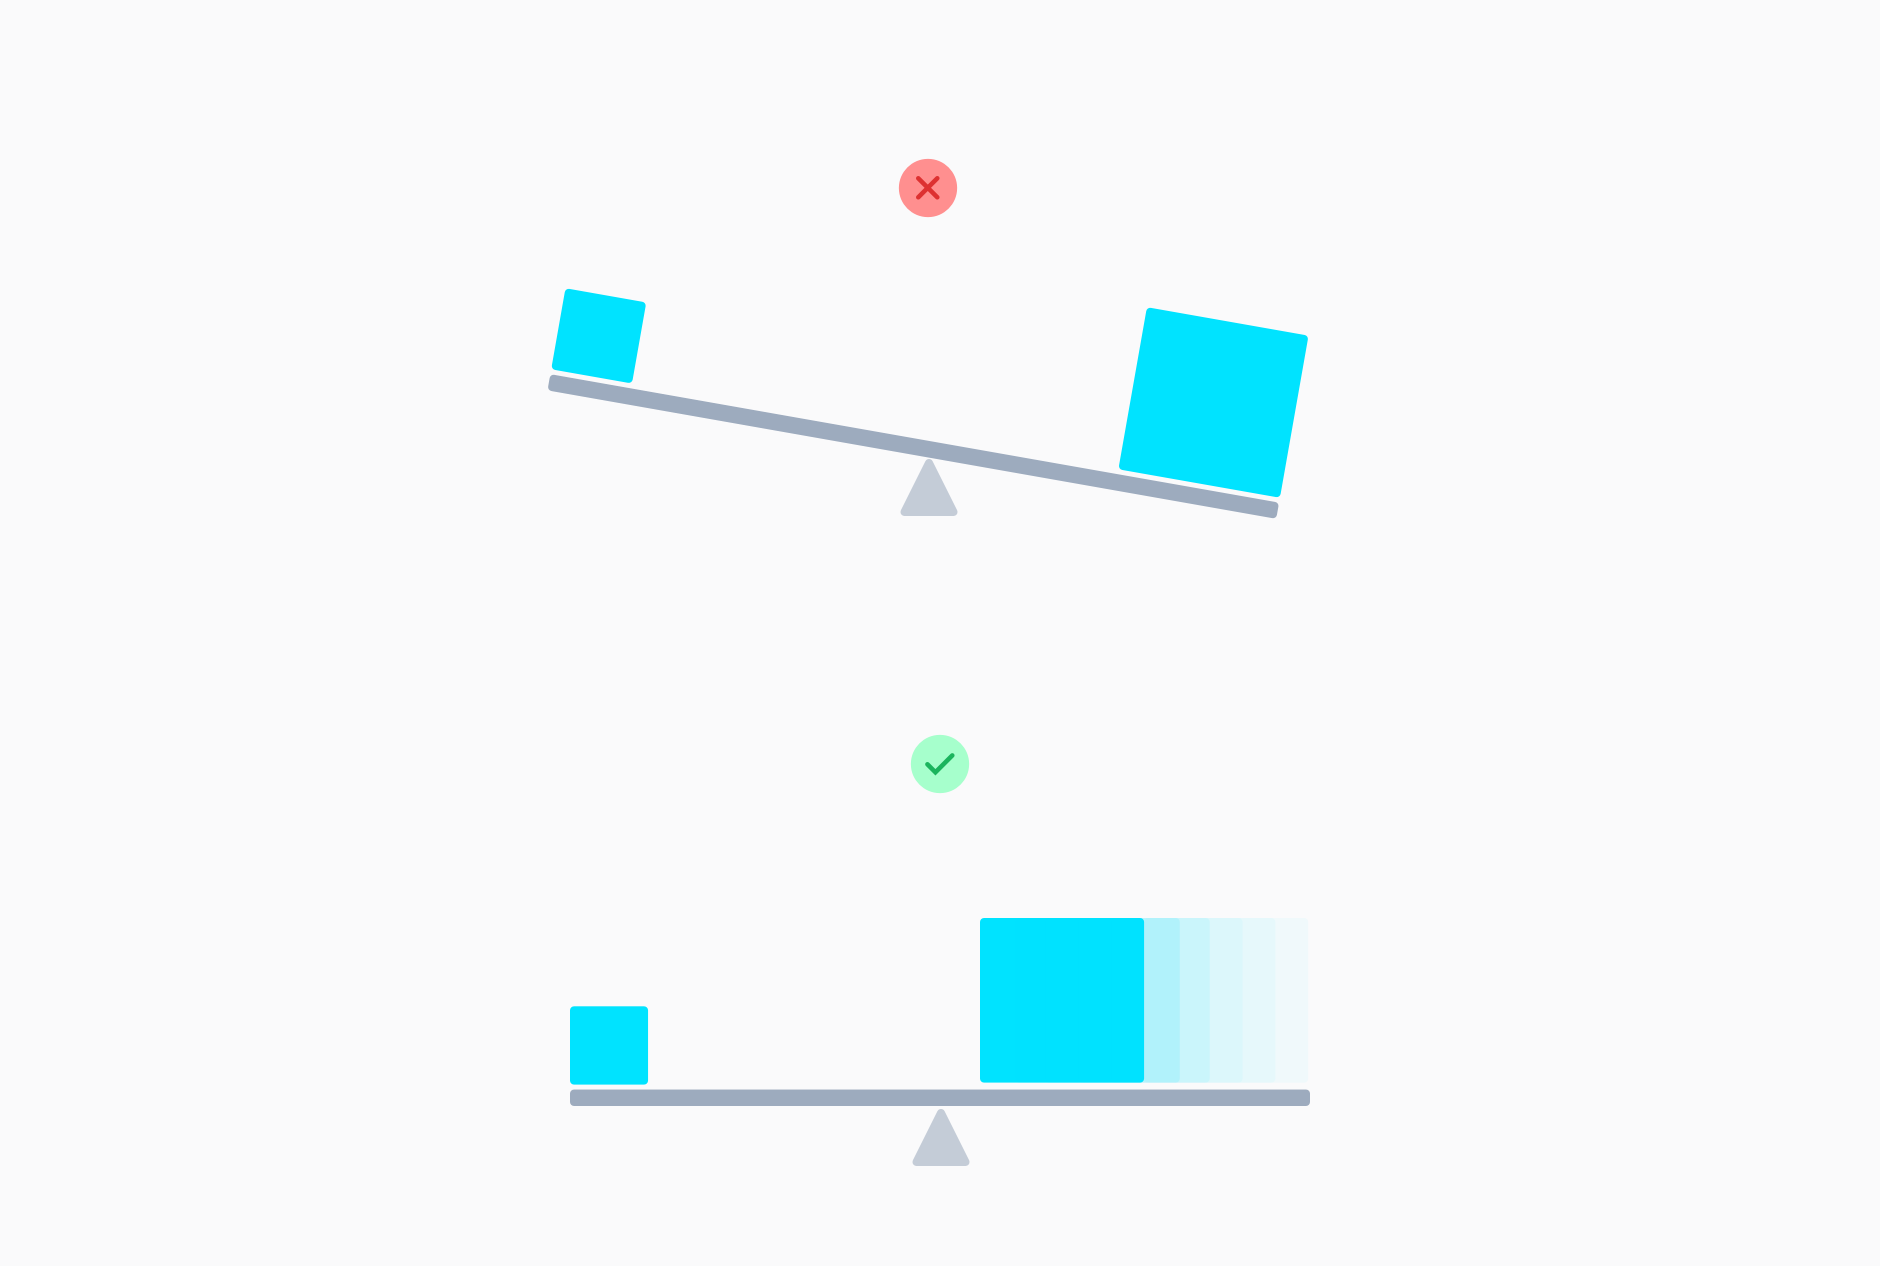
\includegraphics[width=10cm]{obrazky/rovnovaha_paka}\hfill
			\caption{Páka rovnováhy vzhledu. Zdroj: \cite{vizualni_rovnovaha}}
		\end{figure}

		Pokud je tedy nejaký prvek vizuálně těžší než druhý, je dobré lehčímu prvku přidat více bílého prostoru a odsunout
		ho tak od těžšího prvku.
		Tím vznikne rovnováha mezi prvky a celkově přívětivější rozhraní.
		\cite{vizualni_rovnovaha}

		Rozvržení prvků ale není vše a je potřeba myslet i na samotný design.
		Je potřeba definovat jasná pravidla a styly, aby byla zajištěna konzistence.

		Nejdůležitější částí designu je správně připravená paleta barev.
		Bylo potřeba připravit spolu kompatibilní barvy použitelné napříč aplikací.
		Hlavní část palety obsahuje obecné barvy: hlavní prezentovanou barvu použitou na místech, která musí být
		patřičně zvýrazněna a barvy pro různé texty jako hlavní text, nadpis, podnadpis nebo popisek.
		Dále paleta obsahuje paletu obecných základních barev pro případ například uživatelských úprav některých objektů.
		Důležitými barvami jsou i barvy pro označování polí formuláře, zejména pak jejich správnosti při validaci
		hodnot.
		Paleta obsahuje i ostatní méně obecné barvy a je samozřejmě možné ji v budoucnu rozšiřovat, avšak je potřeba se
		vždy zamyslet jestli je nová barva skutečně nutná a zda-li je kompatibilní s již použitými barvami.
		Většina barev je inspirována výše zmíněným Material Designem obsahující širokou paletu barev, kterou lze jednoduše
		využít v jakémkoliv projektu.

		\begin{figure}[H]
			\centering
			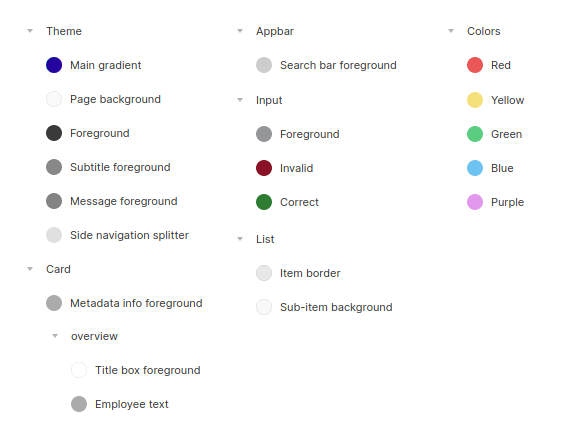
\includegraphics[width=\linewidth]{obrazky/paleta_barev}\hfill
			\caption{Navržená paleta barev. Zdroj: [autor]}
		\end{figure}

		Dalším velmi důležitým designovým prvkem jsou stíny pomáhající vizualizovat pomyslnou vzdálenost jednotlivých
		prvků od uživatelova zraku.
		Díky stínům je totiž možné u více překrývajících se prvků jasně ilustrovat uživateli, které prvky jsou více v
		popředí než ostatní.
		Tím lze zároveň poměrně efektivně odlišit jednotlivé bloky od sebe.
		Způsobů používání stínu je mnoho.
		Pro tento projekt byl vybrán způsob, kdy stín se snaží simulovat reální stín generovaný jedním světelným zdrojem.
		Na takové stíny jsou uživatelé zvyklí z reálného světa a je pro ně jednodušší pochopit oddělení prvků.
		Velmi používané je i využití linek kolem jednotlivých prvků pro oddělení bloků, případně se kombinuje obojí.
		Ve skutečnosti i tento projekt používá kombinaci linek a stínů.
		Stíny jsou v tomto případě použity hlavně pro bloky ucelených informací a prvků které mají vyšší prioritu než
		ostatní v rámci jednoho bloku a linky jsou použity pro standardní prvky uvnitř bloků.
		Kombinace byla vybrána z důvodu zjednodušení vzhledu, protože použití pouze stínů by mohlo pro některé uživatele
		být příliš rozptylující.

		\begin{figure}[H]
			\centering
			
\includegraphics[width=8cm]{obrazky/ukazka_stinu_a_linek}
			\caption{Ukázka kombinace stínů a linek v jednom bloku. Zdroj: [autor]}
		\end{figure}

		Kromě linek a stínu je dobré myslet i na samotné okraje prvků, tj. zda-li budou mít zaoblené rohy a podobně.
		Po vzoru Material Designu byly zvoleny zaoblené rohy o průměru 8px pro větší lehkost prvků.
		Toto rozhodnutí je však celkem subjektivní a někteří uživatelé mohou preferovat ostré rohy.

		\begin{figure}[H]
			\centering
			
\includegraphics[width=8cm]{obrazky/blok_obsahu}\hfill
			\caption{Ukázka zaoblených rohů. Zdroj: [autor]}
		\end{figure}

		Posledním pravidlem je jednotná signalizace výběru.
		Tato část musí být obzvlášť konzistentní napříč aplikací a intuitivní pro koncové uživatele.
		Uživatel musí být schopen jednoznačně určit jaký prvek ze všech možných je vybraný ať už se jedná o navigaci
		nebo výběr položky ve formuláři.
		Velice používaným způsem jak tuto signalizaci řešit je jednoduchá linka zobrazená u vybraného prvku.
		V rámci této aplikace byly navrženy dvě varianty: varianta pro pás prvků a varianta pro samostatné prvky.
		Varianta pro pás prvků se použije v případě pásu prvků, u kterých nemůže dojít k přetečení na více řádků.
		V takovém případě se použije jednoduchá linka pod či nad prvkem.
		V případě osamocených prvků nebo víceřádkových prvků je použita linka kolem celého okraje prvku.

		\begin{figure}[H]
			\centering
			
\includegraphics[width=6cm]{obrazky/ukazka_vyberu_1}\hfill
			\caption{Ukázka signalizace výběru v navigaci. Zdroj: [autor]}
		\end{figure}

		\begin{figure}[H]
			\centering
			
\includegraphics[width=4cm]{obrazky/ukazka_vyberu_2}\hfill
			\caption{Ukázka signalizace výběru konkrétního prvku. Zdroj: [autor]}
		\end{figure}

		Na těchto principech je tedy možné navrhnout nějaké základní univerzální prvky pro tvorbu konkrétních stránek
		a následně celý vzhled.

		\subsubsection{Strukturální prvky}

		Strukturálními prvky jsou myšlené takové prvky, které slouží jako základní stavební prvky pro jednotné
		rozvržení stránek a oddělení prvků uceleným způsobem.
		Tyto prvky tak slouží jako prvky obalovací a bez vnořených interaktivních prvků nedávají samostatně smyl
		a jsou především pomůckou pro tvoření stránek.

			\paragraph{Blok obsahu}

			\begin{figure}[H]
				\centering
				
\includegraphics[width=6cm]{obrazky/blok_obsahu}\hfill
				\caption{Ukázka bloku obsahu. Zdroj: [autor]}
			\end{figure}

			Stránky jsou rozvrženy hlavně pomocí tzv. bloků obsahu označující jeden logický celek informací
			na stránce.
			Blok obsahu vždy obaluje nějaký konkrétní obsah: dlouhý text, seznam položek, editor a cokoliv dalšího.
			Blok obsahuje hlavičku obsahující nadpis popisující logický celek informací, co se bude v bloku nacházet
			a k čemu slouží, a lištu tlačítek dávající smysl pro celý logický celek seřazenou zprava od nejdůležitějších
			akcí.
			Samotný obsah těla už je pak záležitostí konkrétního použití, avšak pravidlem je jednotné odsazení 24px od
			okrajů bloku.
			Krajním případem je využití bloku bez hlavičky na speciálních stránkách s vlastním nadpisem, kde blok
			představuje logický celek informací platných pro celou stránku (příkladem mohou být stránky s popisem
			funkcí aplikace uživateli).

			V případě více logických celků na jedné stránce se použije více bloků řazených pod sebou a oddělených 24px
			pro dostatečné oddělení rozlišných informací.

			\begin{figure}[H]
				\centering
				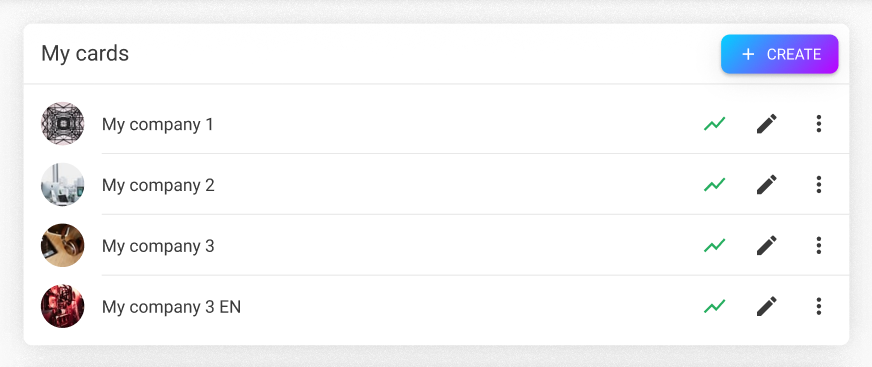
\includegraphics[width=\linewidth]{obrazky/blok_obsahu_ukazka}\hfill
				\caption{Ukázka využití bloku obsahu. Zdroj: [autor]}
			\end{figure}

			Uvnitř bloku se může nacházet jakýkoliv obsah.
			Nicméně je několik základních prvků, které se zde běžně nacházejí a je nutno aby byly konzistentní.
			Jedná se především o seznamy prvků, textová pole a vnitřní logické celky.
			Seznamy prvků definují vlastní odsazení a proto jsou výjimkou nepoužívající standardní vnitřní odsazení
			bloku.
			Dobrým pravidlem je omezit množství seznamů v jednom bloku na jeden, protože více seznamů může představovat
			značné zmatení uživatele.
			Textová pole vlastní odsazení nemají, nicméně pokud takových polí je v jednom bloku více, musí být oddělena
			mezi sebou 16px a horizontálně zobrazovat maximálně dvě pole.
			Ve některých případech je nutné logický celek rozdělit ještě na dílčí celky, většinou pomocí speciálních
			tlačítek odkazujících na jiné stránky.
			Ty po vzoru bloků mají stín pro odlišení od běžných prvků a mezi sebou mají prostor 16px stejně jako
			textová pole.

			\paragraph{Lišta akcí}

			\begin{figure}[H]
				\centering
				
\includegraphics[width=\linewidth]{obrazky/lista_akci}\hfill
				\caption{Ukázka lišty akcí. Zdroj: [autor]}
			\end{figure}

			Kromě hlavní navigační lišty aplikace dostupné téměř na všech stránkách pro jednoduchou navigaci mezi
			částmi aplikace, bylo nutné zavést ještě jeden typ lišt: lišta akcí.
			Díky ní je možné na určitých stránkách zobrazit sekundární lištu s nadpisem a dodatečnými akcemi vztahující
			se k obsahu stránky jako celku.
			Takovými stránkami jsou většinou stránky zobrazující detail určitého jednoho objektu, který lze například
			smazat nebo upravit, ale zároveň je potřeba zobrazit vnořená data (příkladem může být editor jedné karty).
			Navíc může obsahovat i sekundární navigaci spojenou s konkrétním objektem.

			\paragraph{Modální okno}

			\begin{figure}[H]
				\centering
				
\includegraphics[width=\linewidth]{obrazky/modalni_okno}\hfill
				\caption{Ukázka modálního okna. Zdroj: [autor]}
			\end{figure}

			Modální okna představují bloky obsahu překrývající všechen ostatní obsah při zobrazí, aby se uživatel zaměřil
			pouze na obsah uvnitř okna a nebyl rušen zbylým obsahem, který v danou chvíli není důležitý.
			Jedná se především o potvrzení určité akce vyvolané uživatelem nebo zobrazení detailu nějakého dílčího prvky.
			Modální okno se může zobrazit pouze jako reakce na uživatelskou akci, nesmí dojít k samovolnému zobrazování
			náhodných oken, protože to vede k frustraci uživatele.
			Každé okno má hlavičku a případně i patičku, avšak obsah se mění podle typu okna.
			Tato aplikace rozlišuje dva primární typy oken: informační okno a akční okno.
			Informační okno slouží pouze k zobrazení již existujících dat a nevyžaduje od uživatele žádnou akci.
			Lze ho zavřít buď křížkem v hlavičce nebo kliknutím mimo okno a neobsahuje patičku.
			Akční okno akci vyžaduje a uživatel musí vždy nějakou akci zvolit, nelze okno zavřít pouhým kliknutím mimo okno.
			Takové okno má v hlavičce pouze nadpis a obsahuje patičku se všemi možnými akcemi, které uživatel může provést.
			Akce jsou většinou dvě a jsou seřazeny zprava od té nejdůležitější.
			Příkladem takových akcí může být potvrzení vytvoření objektu a zrušení akce.
			U tohoto typu okna se navíc předpokládá, že bude obsahovat kromě statických i nějaký formulář, který musí
			uživatel vyplnit, není to však pravidlem.
			Tlačítko nejdůležitější akce by mělo být patřičně odlišeno od běžných tlačítek, aby bylo zřejmé co se po
			uživateli chce.

			Okna mají podobná pravidla odsazení jednotlivých vnitřních prvků jako bloky obsahu.
			Obsah by měl být odsazen 24px od okrajů okna (až na výjimky s vlastním odsazením) a akční tlačítka jsou
			mezi sebou odsazeny 8px.
			Celá patička je navíc od samotného obsahu taktéž odsazena 24px pro jasné rozdělení částí.

			\begin{figure}[H]
				\centering
				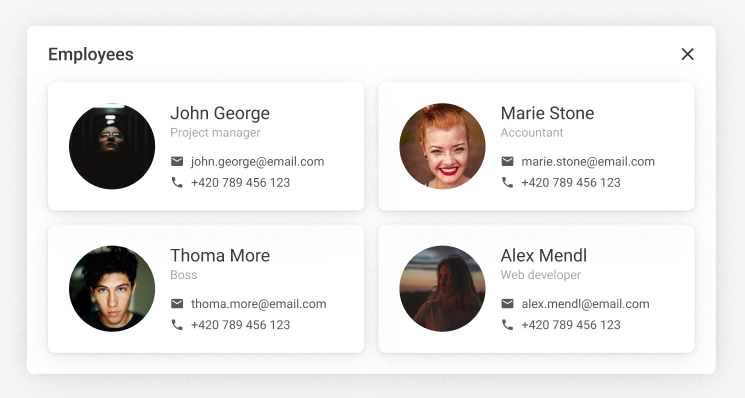
\includegraphics[width=10cm]{obrazky/modalni_okno_informacni_ukazka}\hfill
				\caption{Ukázka konkrétního informačního modální okna. Zdroj: [autor]}
			\end{figure}

			\begin{figure}[H]
				\centering
				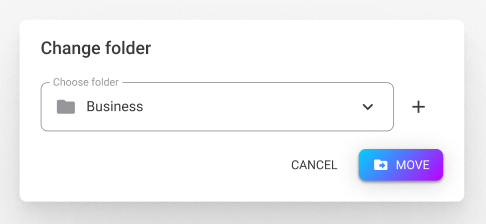
\includegraphics[width=10cm]{obrazky/modalni_okno_akcni_ukazka}\hfill
				\caption{Ukázka konkrétního akčního modálního okna. Zdroj: [autor]}
			\end{figure}

			\paragraph{Kontextuální nabídka}

			\begin{figure}[H]
				\centering
				
\includegraphics[width=6cm]{obrazky/kontextualni_nabidka}\hfill
				\caption{Ukázka kontextuální nabídky. Zdroj: [autor]}
			\end{figure}

			Jedná se malé menu zobrazující rozšířené možnosti nějaké akce.
			Většinou se používá pro zobrazení vícero akcí možných nad nějakým objektem, pokud není v \ac{UI} dostatek
			místa pro všechny akce nebo pro výběr konkrétní položky výběrového pole ve formuláři.
			Nabídka podobně jako modální okno překrývá část obsahu pro zviditelnění, nicméně ji lze jednoduše zavřít
			kliknutím mimo nabídku.

			\begin{figure}[H]
				\centering
				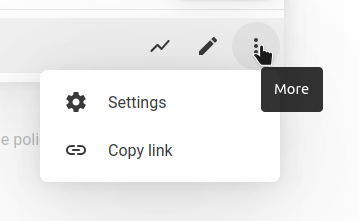
\includegraphics[width=8cm]{obrazky/kontextualni_nabidka_seznam_ukazka}\hfill
				\caption{Ukázka kontextuální nabídky akcí položky v seznamu. Zdroj: [autor]}
			\end{figure}

			\begin{figure}[H]
				\centering
				
\includegraphics[width=8cm]{obrazky/kontextualni_nabidka_vyberove_pole_ukazka}\hfill
				\caption{Ukázka kontextuální nabídky položek výběrového pole. Zdroj: [autor]}
			\end{figure}

			\paragraph{Sekce}

			\begin{figure}[H]
				\centering
				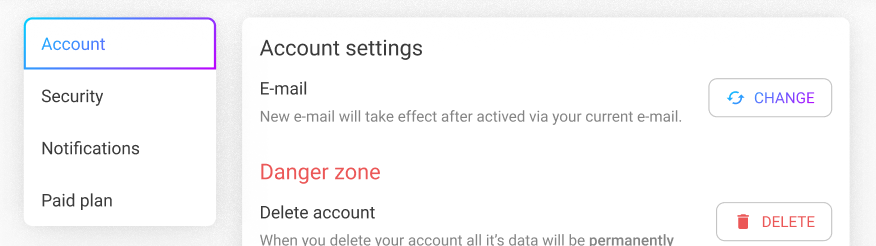
\includegraphics[width=\linewidth]{obrazky/sekce}\hfill
				\caption{Ukázka sekce. Zdroj: [autor]}
			\end{figure}

			Pro stránky složené z více podstránek (např.: nastavení uživatelského účtu) je vhodné provázat tyto stránky
			nějakou navigací pro jednoduchý přechod mezi dílčími stránkami.
			K tomu slouží extenze bloku obsahu o postranní menu sloužící právě pro navigaci souvisejících stránek.
			Díky viditelnému menu je jasně viditelné jako sekce jsou uživateli dostupné a co tak uživatel může vše dělat.

		\subsubsection{Prvky pro interakci}

		Po prvcích strukturující obsah je možné navrhnout již prvky, se kterými bude uživatel přímo či nepřímo interagovat.

			\paragraph{Tlačítko}

			Nejhlavnějším takovým prvkem je tlačítko.
			To umožňuje uživatelům vyvolávat akce, potvrzovat akce nebo se nechat přesměrovat na jiné stránky.
			Tlačítek je v aplikaci spousta a každé dělá trochu něco jiného.
			Lze je ale zařadit do pár kategorií a navrhnout tak pár typů tlačítek evokující jejich prioritu a vážnost akce,
			se kterou jsou spojeni.
			Všechny tlačítka byla rozdělena na tlačítka s nízkou prioritou, tlačítka s vysokou prioritou a tlačítka s vysokou
			prioritou a vysokou vážností akce.

			Tlačítko s nízkou prioritou reprezentuje vedlejší akci, kterou sice uživatel může provést, ale není hlavním cílem.
			Takové tlačítko má neutrální barvu a ve většině případech neobsahuje ani ikonu, aby nevyjadřovalo vysokou prioritu
			a uživatel se zaměřil spíše na výraznější tlačítka.

			\begin{figure}[H]
				\centering
				
\includegraphics[width=4cm]{obrazky/tlacitko_s_malou_prioritou}\hfill
				\caption{Ukázka tlačítka s malou prioritou. Zdroj: [autor]}
			\end{figure}

			Tlačítko s vysokou prioritou představuje primární akci, kterou by se uživatel měl vydat.
			Taková tlačítka představují potvrzení nějaké akce, vytvoření nových objektů, přidání existujících objektů a
			podobně.
			Měli by být proto patřičně zvýrazněna a uživatele podvědomě navést kam má kliknout pokud v danou akci chce
			provést.
			Tato tlačítka mají proto výraznou barvu a vystihující ikonu pro zpřehlednění a zpříjemnění celkového dojmu.

			\begin{figure}[H]
				\centering
				
\includegraphics[width=4cm]{obrazky/tlacitko_s_velkou_prioritou}\hfill
				\caption{Ukázka tlačítka s vysokou prioritou. Zdroj: [autor]}
			\end{figure}

			Pro případy kdy uživatel provádí nějakou akci s vysokou vážností jako je například nevratné smazání nějakého
			objektu, vzniklo rozšíření tlačítka s vysokou prioritou.
			Tlačítko se lišší pouze v červené barvě evokující dojem závažné akce.
			Právě červená barva by měla uživatele přimět znovu zamyslet se nad prováděnou akcí, protože červená barva
			je využívána jako symbol něčeho negativního.

			\begin{figure}[H]
				\centering
				
\includegraphics[width=4cm]{obrazky/tlacitko_s_velkou_prioritou_a_velkou_vaznosti}\hfill
				\caption{Ukázka tlačítka provádějící nevratnou změnu. Zdroj: [autor]}
			\end{figure}

			\paragraph{Vstupní pole}

			Vstupní pole různých druhu jsou společně s tlačítky nejdůležitějšími prvky jakékoliv aplikace.
			Vstupní pole umožňují uživatelům předat data aplikaci v různých formátech podle požadované informace.
			Vzniklo proto několik základních typů vstupních polí, které lze jednoduše kombinovat uvnitř v formulářů.
			Mezi ně patří: textové pole, výběrové pole, pole pro výběr času a data, pole pro nahrání obrázku a pole pro
			výběr geografické lokace.
			Vstupní pole využívají linek namísto stínu, protože sami o sobě nereprezentují celek ale pouze část celého
			bloku.
			Pole mají popisek pro identifikaci účelu konkrétního pole, ikonu a mohou mít i akční tlačítko pro jednoduchou
			akci nad danou zadanou hodnotou.
			U většiny polí je navíc popisek plovoucí, kdy pokud pole nemá žádnou hodnotu, nahradí ji popisek, pokud však
			nějaká hodnota byla zadána, popisek se zmenší a posune stranou, aby zůstal stále viditelný, ale nepřekážel.
			Pole jsou také schopna změnit svoji barvu a zobrazit popis chyb, pokud je zadaná hodnota nevalidní.
			Pokud je hodnota validní nebo žádná ještě neexistuje, je možné na místo chyby pod pole vepsat nápovědu k danému
			poli pro koncového uživatele v případě nejasných polí nebo potřebě dodatečných informací v podobě například
			požadovaného formátu.

			Textové pole slouží pro zadávání různých krátkých i dlouhých textů, mají vždy popisek a mohou mít ikonu a
			akční tlačítko.
			Mohou sloužit i pro zadávání hesel a v takovém případě zobrazují pouze zástupné znaky.
			Obsahují však tlačítko pro přepnutí mezi zástupnými znaky a originálními pro kontrolu zadaného hesla.

			\begin{figure}[H]
				\centering
				
\includegraphics[width=8cm]{obrazky/textove_pole}\hfill
				\caption{Ukázka textového pole s ikonou a nápovědou. Zdroj: [autor]}
			\end{figure}

			Extenzí textového pole jsou pole pro zadání času a data.
			Ty rozšiřují manuální zadávání o okénka pro pohodlný výběr bez nutnosti klávesnice.

			\begin{figure}[H]
				\centering
				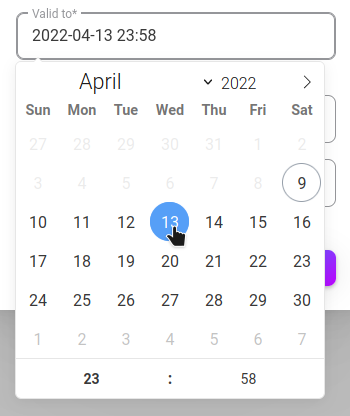
\includegraphics[width=6cm]{obrazky/datumove_pole}\hfill
				\caption{Ukázka pole s výběrem data a času. Zdroj: [autor]}
			\end{figure}

			Vzhledem k požadavku možnosti specifikovat geografické lokace karet bylo potřeba zavést i specifické pole
			pro výběr bodu v mapě.
			Pole zobrazuje automaticky mapu světa, kterou je možné hýbat a přibližovat ji a vybírat konkrétní body.
			Vybraný bod lze také jednoduše smazat/resetovat.
			Na rozdíl od textového pole toto pole neumožňuje specifikovat ikonu ani akční tlačítko a obsahuje pouze
			statický popisek kvůli stále zobrazené mapě do všech krajů.

			\begin{figure}[H]
				\centering
				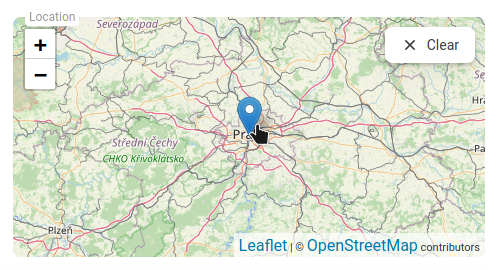
\includegraphics[width=8cm]{obrazky/pole_lokace}\hfill
				\caption{Ukázka pole pro výběr geografického bodu v mapě. Zdroj: [autor]}
			\end{figure}

			Posledním méně používaným polem v této aplikaci je pole pro výběr obrázku.
			Pole umožní výběr souboru ze souborového systému uživatele, který je následně nahrát a zobrazen jeho náhled
			přímo v poli.
			Vybraný obrázek je pak možné jednoduše změnit nebo úplně odstranit.

			\begin{figure}[H]
				\centering
				
\includegraphics[width=5cm]{obrazky/obrazkove_pole}\hfill
				\caption{Ukázka pole s nahraným obrázkem. Zdroj: [autor]}
			\end{figure}

			\paragraph{Seznam položek}

			Velmi využívaným prvkem je seznam jakýchkoliv položek.
			Seznam může být jednoduchý pouze pro jednoduché zobrazení několika podobných položek nebo může umožňovat
			spravovat objekty stejného typu pomocí přidělených akcí a dodatečných informací.
			Samotný seznam je pouze obalovací prvek, až prvky konkrétních položek obsahují pokročilé možnosti.
			Každá položka může obsahovat ikonu nebo obrázek, text, seznam akcí nebo dokonce i vnořený seznam dílčích
			položek stahujících se k dané nadřazené položce.
			Nicméně vnořené seznamy jsou omezeny pouze na jednu úroveň kvůli zachování přehlednosti, více úrovní navíc
			běžně není potřeba a u takového scénáře by bylo na zvážení zda-li je vícenásobné vnoření tím správným řešením.
			Seznamy akcí se kromě běžného zobrazení umí i seskupit v případě malého místa a schovat akce do kontextuální
			nabídky, aby uživatel využívající malé zařízení nepřišel o možnost využívat všechny akce s minimálním omezením.

			\begin{figure}[H]
				\centering
				
\includegraphics[width=8cm]{obrazky/jednoduchy_seznam}\hfill
				\caption{Ukázka jednoduchého seznamu podobných prvků. Zdroj: [autor]}
			\end{figure}

			\begin{figure}[H]
				\centering
				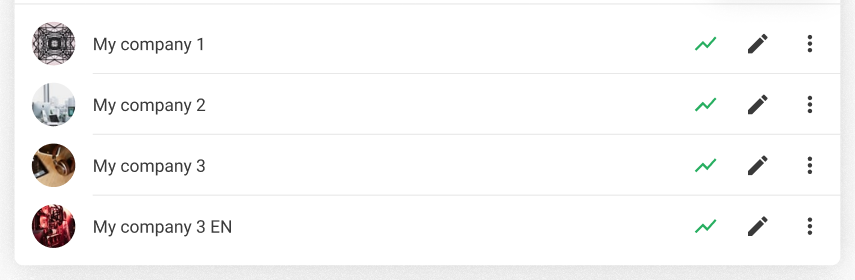
\includegraphics[width=\linewidth]{obrazky/seznam}\hfill
				\caption{Ukázka pokročilého seznamu prvků. Zdroj: [autor]}
			\end{figure}

			\begin{figure}[H]
				\centering
				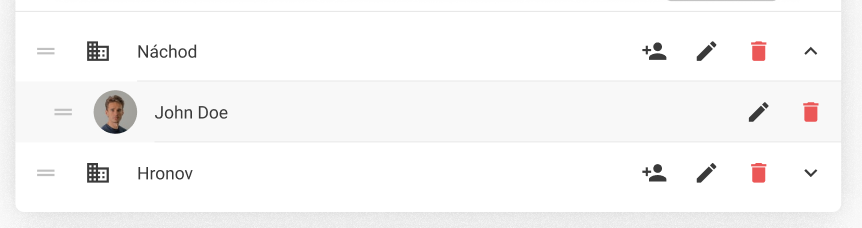
\includegraphics[width=\linewidth]{obrazky/vnoreny_seznam}\hfill
				\caption{Ukázka vnořeného seznamu uvnitř jiného seznamu. Zdroj: [autor]}
			\end{figure}

			\paragraph{Stránkování}

			Při velkém množství položek v jednom seznamu je běžně používaný systém stránkování, kdy se položky rozdělí
			do stránek s omezeným počtem prvků pro jednodušší navigaci po stránce bez nutnosti příliš pohybovat myší.
			Prvek stránkování umožňuje přepínat mezi konkrétními stránkami nebo se přepínat mezi předchozí a následující.
			Pokud je velké množství stránek, prvek nezobrazí všechny stránky, ale zobrazí pouze okolí vybrané stránky
			a první a poslední stránky pro rychlou navigaci.

			\begin{figure}[H]
				\centering
				
\includegraphics[width=4cm]{obrazky/strankovani}\hfill
				\caption{Ukázka stránkování. Zdroj: [autor]}
			\end{figure}

		\subsubsection{Finální návrh}

		S pomocí výše navržených základních prvků a jejich variacemi bylo navrženo finální \ac{UI} všech stěžejních
		stránek.

		\begin{figure}[H]
			\centering
			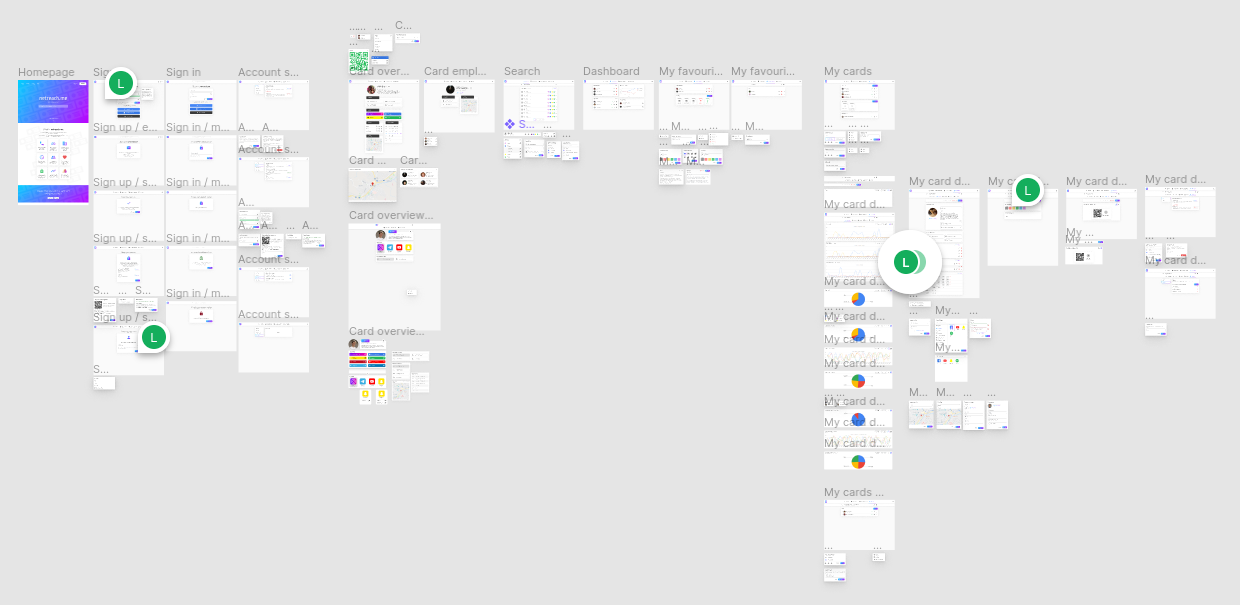
\includegraphics[width=\linewidth]{obrazky/finalni_navrh}\hfill
			\caption{Finální grafický návrh aplikačních stránek a prvků. Zdroj: [autor]}
		\end{figure}

		Tento postup s návrhem aplikace před samotnou aplikací se ukázal jako velmi efektivní oproti původnímu prototypu
		pomohl nejen snadněji implementovat samotné \ac{GUI}, ale i navrhnout \ac{API} díky zřetelným požadavkům na
		manipulaci s daty.
		\ac{API} tak bylo částečně navrženo právě podle designového návrhu, protože návrh mimo jiné umožnil realizovat
		vizi požadavků na \ac{UI} i funkce aplikace.

	\subsection{Implementace API serveru}

		\subsubsection{Datový model}

		Úkol API serveru je poskytovat a zpracovávat data ať už textová v pobobě \ac{JSON} dokumentů nebo binární v podobě
		obrázků.
		Tyto funkce pro samotné API bude zprostředkovávat implementovaná business logika starající se, aby všechna data
		byla správně zpracována.
		Je ale stěžejní se na počátku zamyslet a vybrat styl a navrhnout model jakým bude business logika implementována.
		Stěžejní je to z důvodu budoucí čitelnosti kódu a možnostech rozšíření o nové funkce, protože při špatném
		návrhu může být složité aplikace rozšířit a kód se tak může stávat postupně nečitelným.

		Vzhledem k tomu, že byl vybrán jazyk Java, který je primárně objektově orientovaný programovací jazyk, business
		logika bude využívat právě objektově orientovaného programování \ac{OOP}.
		\ac{OOP} je velice populární a většinově používané obecné programovací paradigma využívané spousty programovacími
		jazyky.
		Toto paradigma využívá objekty pro reprezentaci celého systému (aplikace).
		Každý objekt má nějaké své vlastnosti a operace, které může buď využívat vnitřně nebo poskytnou k využití ostatním
		objektům.
		Hlavní myšlenka \ac{OOP} je popisovat reálné objekty (člověk, pes, budova, událost...) těmi virtuálními ve zjednodušené
		formě, kdy popisujeme jen tu část reálného objektu, která nás zajímá.
		Tyto objekty pak v systému mezi sebou komunikují pomocí zpráv a předávají si data, tak aby dosáhli výsledku
		očekávaného od celého systému.
		Každý objekt v systému má svou předlohu zvanou třída definující pro každý objekt jako vlastnosti a operace daný objekt
		může obsahovat a objekt je pak už konkrétní instance obsahující konkrétní data.
		Kromě tříd ještě existují rozhraní a abstraktní třídy, které můžou mezi sebou dědit vlastnosti a operace a z nich
		následně vznikají konkrétní třídy.
		Rozhraní a abstraktní třídy definují obecnou předlohu operací, tzv. kontrakt, který dědící třída musí splňovat, což
		následně umožňuje využít techniku polymorfismus, tj. provádět operace na základě obecného rozhraní bez nutnosti
		vědět konkrétní a třídu a její chování.
		\cite{oop}

		Právě díky \ac{OOP} bylo možné poměrně věrně reprezentovat objekty využívané jednotlivými stránkami v logické,
		přehledné a jasně definované struktuře.
		Model navrhovaného systému původně vycházel z modelu použitém v prototypu, avšak po hlubší analýze požadavků byl
		značně přepracován.
		Nový model byl pro přehlednost interně rozdělen na několik modulů podle jejich zaměření, nicméně všechny moduly
		mezi sebou i tak komunikují, ale nejsou spolu hluboce provázány.
		Momentálně se datový model skládá z modulu pro správu uživatelských účtů, modulu pro správu karet, modulu pro správu
		kupónů pro prémiové plány a podpůrného modulu.

		Modul uživatelských účtů je zodpovědný za vytváření, uchování, úpravu a mazání jednotlivých účtů a jejich dat
		každého jednoho uživatele.
		S tím je spojena i správa oblíbených karet a poznámek, které jsou vždy na konkrétního uživatele a propojují
		moduly účtů a karet.
		Modul dál řeší i prémiový plán a předplatné.

		\begin{figure}[H]
			\centering
			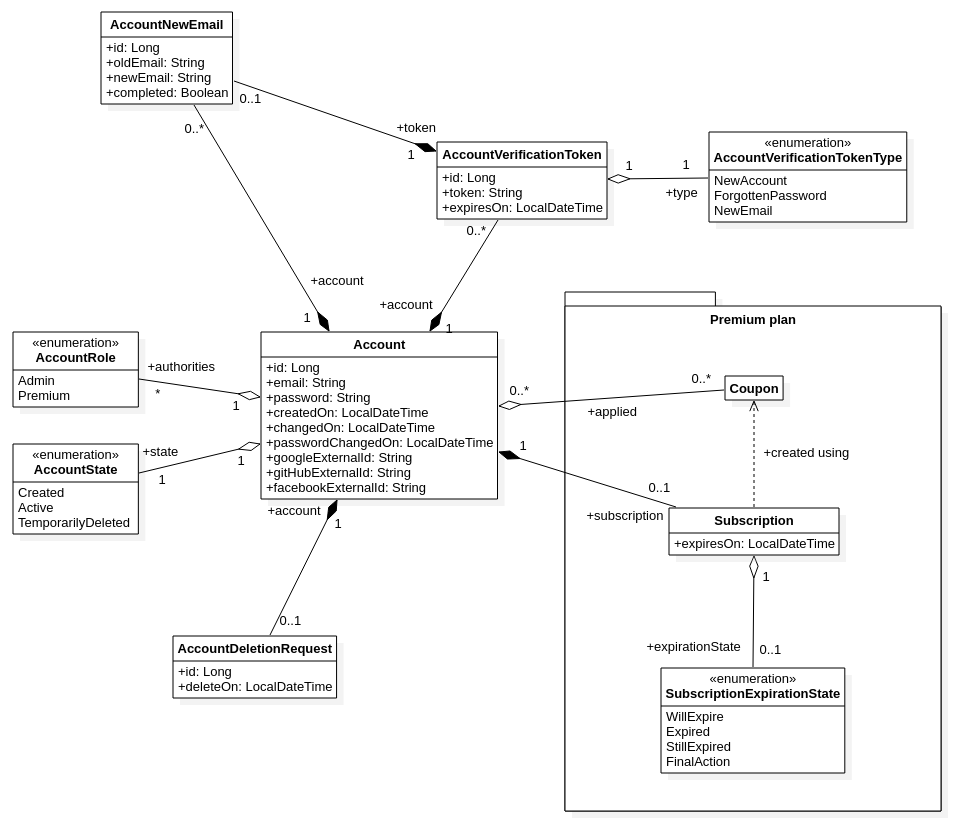
\includegraphics[width=\linewidth]{obrazky/datovy_model_ucet}\hfill
			\caption{Datový model popisující uživatelské účty. Zdroj: [autor]}
		\end{figure}

		Jak je možno vidět z diagramu, účet má kromě základních přihlašovacích informací v pohodě buď běžné kombinace emailové adresy
		a hesla nebo v podobě externích poskytovatelů externích uživatelských účtů, i spoustu
		doplňujících rozšiřujících tak možnosti.

		V první řadě, každý účet má přiřazený vždy nějaký stav.
		Při vytvoření má nový účet stav \emph{Created} vyjadřující nový a zatím neaktivovaný účet.
		Tento účet nelze využívat.
		Po aktivaci účtu se změní stav na \emph{Active}, který říká, že účet je již aktivovaný a tedy plně použitelný.
		Poslední stav \emph{TemporarilyDeleted} označuje účet dočasně smazaný, což znamená, že je naplánováno jeho permanentní
		smazání.
		Do tohoto stavu se účet dostane na uživatelovu žádost o smazání svého účtu a zajišťuje, že uživatel může v omezené
		lhůtě svůj účet zase obnovit, pokud by si žádost rozmyslel.

		Další velmi důležitou komponentou je systém ověřovacích tokenů sloužící k potvrzování různých uživatelských akcí, kde
		je potřeba ověřit, že akci provádí skutečný uživatel nikoliv podvodník.
		Tokeny jsou pseudo náhodně generované unikátní textové řetězce přiřazené vždy k jednomu určitému uživateli.
		Typ tokenu pak říká co daný token ověřuje.
		Ověřovanou akcí může být aktivace nového účtu, změna emailové adresy nebo zapomenuté heslo.
		Tyto tokeny jsou zasílány uživateli na jeho emailovou adresu což zaručí, že přístup k danému tokenu má pouze skutečný
		vlastník (emailová adresa slouží jako zdroj věrohodnosti).
		V případě tokenu pro změnu emailové adresy se nová emailová adresy se ukládá mimo samotný účet k danému tokenu.
		Díky tomu je možné emailovou adresu změnit až ve chvíli kdy byl token skutečně ověřen a zároveň je možné držet
		historii všech změn emailů pro zpětné dohledání v případě například odcizení účtu.

		Systém dále na několika místech pracuje s tzv. rolemi udávajícími obecná práva daného uživatele.
		Každé obecné roli jsou přiřazena nějaká práva v systému (čtení, modifikace...), a pokud uživatel má takovou roli
		přiřazenou, automatický dědí její práva.
		Toto je poměrně jednoduchý a efektivní systém práv.
		Momentálně systém pracuje s administrátorskou rolí a prémiovou rolí.
		Administrátorská role uděluje uživateli práva pro přístup do interní administrační části
		aplikace, pomocí které je možné spravovat samotný provoz aplikace.
		Tato role je určená výhradně pro správce aplikace, nikoliv pro běžné uživatele a je přiřazována ručně specifických
		uživatelům.
		Druhou rolí je role prémiová, která již určená pro běžné uživatele je a odemyká jim prémiové funkce aplikace.
		Tato role vzniká automaticky při vytvoření předplatného a zaniká s jeho expirací.

		Pro zmiňované plánované smazání účtu se uchovává požadavek s informací o jaký účet se jedná a kdy dojde k permanentnímu
		smazání daného účtu společně s jeho daty.
		Tyto požadavky jsou následně pravidelně kontrolovány zda-li již by měl daný účet být smazán.

		Poslední hlavní částů uživatelských účtů jsou komponenty pro prémiové funkce.
		Jedná se především o popisný objekt předplatného.
		Ten vzniká při přechodu na prémiový plán a jeho říká, že účet je má předplacený prémiový plán a má proto práva pro
		jinak uzamknuté funkce.
		V jistých případech může mít přiřazený datum expirace, se kterým automaticky zanikne.
		S tím se váže i stav expirace, která pomáhá upozorňovat uživatele na současný stav předplatného.

		\begin{figure}[H]
			\centering
			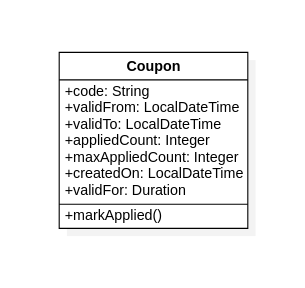
\includegraphics[width=6cm]{obrazky/datovy_model_kupon}\hfill
			\caption{Datový model kupónového systému. Zdroj: [autor]}
		\end{figure}

		Předplatné může vzniknout na základě zadání platného kupónu uživatelem, avšak systém kupónů je navržen obecně, aby
		bylo možné ho v případě budoucích rozšíření jednoduše přepoužít i na aktivaci jiných funkcionalit než jen
		prémiové plány.
		Každý kupón musí mít unikátní kód, buď pseudo náhodně vygenerovaný nebo zadaný správcem.
		Mimo to má definovanou platnost, aby bylo možné tvořit i tzv. "akční" kupóny pouze na dané období, maximální počet
		možných aplikování různými uživateli a doba po jakou bude vytvořené předplatné platné.

		\begin{figure}[H]
			\centering
			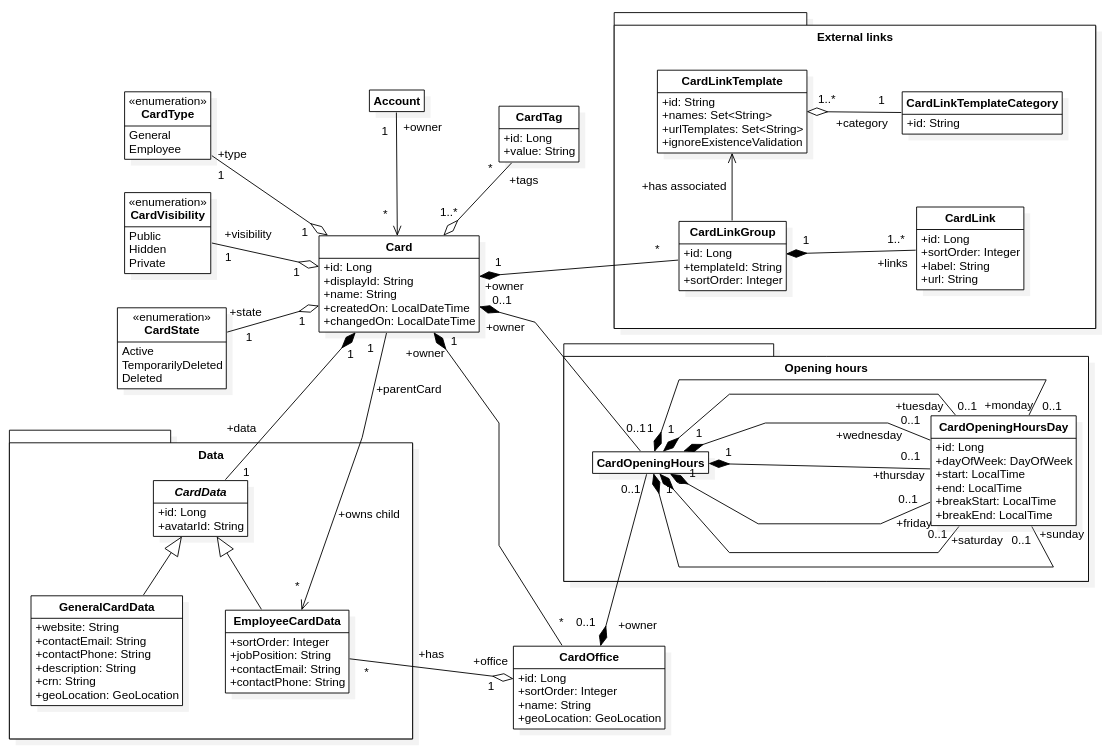
\includegraphics[width=\linewidth]{obrazky/datovy_model_karta}\hfill
			\caption{Datový model karet a navázaných dat. Zdroj: [autor]}
		\end{figure}

		Nejhlavnějším prvkem v této aplikaci jsou samotné karty a jejich data.
		Každá karta má v prvé řadě vždy nějakého vlastníka v podobně uživatelského účtu, který má jako jediný práva na
		úpravu.

		Samotná karta je rozpadnuta do několika částí pro potřebnou modulárnost udávanou více typy karet a různorodostí
		navázaných dat.
		Srdcem je jednoduchá třída popisující pouze obecné metadata, která jsou potřeba pro všechny typy karet.
		V této třídě je tedy zahrnut vlastník, typ, viditelnost, stav, veřejné jméno, tzv. "display ID" a další metadata.
		Display ID je unikátní textové ID karty určené primárně pro koncové uživatele.
		Toto ID je totiž zobrazováno v \ac{URL} adrese konkrétní karty a má za cíl umožnit jednoduše sdílet karty bez nutnosti
		znát kryptické náhodně generované číselné identifikátory.
		Toto ID je může být definováno ručně uživatelem podle jeho libosti (musí však splňovat unikátnost) nebo pseudo
		náhodně generováno aplikací (vhodné pro skryté karty).
		Typ karty definuje jak s danou kartou lze pracovat a jaká data poskytuje.
		Momentálními typy jsou obecná karta a karta zaměstnance, avšak tento systém dovoluje poměrně jednoduché rozšiřování
		o nové typy karet.
		Obecné karty je možné tvořit uživateli přímo a obsahují největší množství informací, protože nedefinují konkrétní
		využití.
		Původně byl tento typ rozdělen ještě na osobní a firemní kartu, nicméně jediný rozdíl bylo omezení podporovaných dat
		v osobních kartách, protože v tomto typu nedávali smysl.
		Tento přístup však přinášel mnoho duplicit a zároveň znemožňoval uživatelům osobních karet využívat funkce
		firemních karet, které ale za určitých okolností dávají smysl i u osobních karet (např.: pro OSVČ).
		Právě kvůli těmto nevýhodám a žádným jasným výhodám, byly tyto dva typy sjednoceny, především pro pohodlí
		koncových uživatelů.
		Karty zaměstnanců se pak tvoří nepřímo jako hierarchické děti obecné karty přímo v editaci nadřazené karty a
		obsahují specifická data pouze pro zaměstnance.
		Posledním důležitým metadatem je viditelnost specifikující kdo může danou kartu vidět.
		Veřejné karty může navštívit a vyhledat kdokoliv.
		Skryté může navštívit pouze uživatel disponující konkrétní \ac{URL} adresou odkazující na dano kartu.
		Privátní kartu pak už slouží pouze pro autora karty.

		Každé kartě lze přiřadit libovolné množství štítků pro jakousi kategorizaci dané karty.
		Štítky jsou uživatelsky definované a můžou tak obsahovat cokoliv, a jsou znovupoužitelné, takže více karet může
		být označeno stejným jedním štítkem.

		Pro definování informací o kartě existuje koncept napojených dat.
		Tyto data reprezentuje soubor informací, které daný typ karty podporuje zadat.
		Každý typ karty má svoji implementaci těchto dat definující podporované informace pro daný typ.
		Je pak business logice aplikace aby dokázala s daty správně pracovat podle typu karty, který je vždy specifikovaný mezi
		základními metadata karty.
		Tato obecnost umožňuje jednoduše vytvářet nové typy karet s úplně odlišnými daty, aniž by se data musela míchat
		a být nepřehledná.

		Pro většinu reálných obecných karet pak pravděpodobně nejdůležitějšími daty budou \ac{URL} odkazy na externí webové stránky,
		především na sociální sítě.
		Ty z karet dělají jakési rozcestníky pro objevení profilů subjektů na sociálních sítích, které koncové uživatele zajímají.
		Každý jeden odkaz má originální cílovou \ac{URL} adresu, popisek a pořadí mezi ostatními odkazy na stejné úrovni.
		Popisek slouží především pro odlišení více odkazů vedoucí na stejnou webovou stránku, nicméně uživatel může popisek
		využít libovolně.
		\ac{URL} adresa je ta hlavní informace a z důvodu bezpečnosti musí být validována oproti zvolené šabloně sítě.
		Díky tomu není možné vytvořit odkaz pod jednou sítí ale odkazovat na podvodnou.
		Jednotlivé odkazy jsou pak seskupovány do skupin odkazů vycházející ze stejné šablony a určují typ šablony pro vše
		vnořené odkazy.
		I přes to, že skupiny zastřešují vždy nějaký soubor sítí stejného typu, může existovat více skupin vycházející ze
		stejné šablony.
		To umožňuje poměrně velkou flexibilitu struktury odkazů a neomezuje uživatele na jeden odkaz pro jednu síť (což je
		nevýhoda některých konkurenčních řešení).
		Jednotlivé šablony jsou reprezentovány separátními konfiguračními třídami udržující definovanou aktuální konfiguraci
		dané šablony pro potřeby business logiky.
		Z návrhu vyplývá potřeba definovat názvy podle kterých lze šablony vyhledat uživateli a platné šablony \ac{URL} odkazů
		oproti kterým se validují konkrétní cílové \ac{URL} adresy.
		Podpora pro možnost definovat více názvu, i přes to že webové stránky mají většinou pouze jeden oficiální název,
		vyplývá z faktu, že mezi uživateli jsou většinou nějaké zažité zkratky názvů daných stránek a očekávají najití
		správné šablony i pod neoficiální zkratkou.
		Stejně jako názvů může být i více šablon \ac{URL} adres, protože většina webových stránek podporuje více domén třetího řádu
		a je tak nutné definovat všechny, protože není jasné jakou \ac{URL} adresu uživatel zrovna zadá.
		Každá taková šablona je pak zařazena do jedné nebo více kategorií sloužící čistě pro jednodušší vyhledávání uživateli
		a momentálně nemá žádné jiné interní využití.

		Pro firmy poměrně užitečnou informací může být jejich hierarchie poboček a zaměstnancům, zejména u větších společností.
		Proto každá obecná karta může mít libovolné množství přiřazených poboček/kanceláří/prodejen, kde každá má své jméno
		a geografickou lokaci pro snadné nalezení uživateli na mapě.
		Ke každé takové pobočce je možné přiřadit zaměstnanecké karty reprezentující jednotlivé zaměstnance setrvávájící
		na dané pobočce.
		Kromě zaměstnanců může mít pobočka přiřazenou i vlastní otevírací dobu.

		Velmi důležitou informací pro potencionální zákazníky je aktuální otevírací doba, ať už se jedná o samotnou kartu nebo
		jen pobočku.
		Byl proto navržen obecný model otevírací doby, který lze navázat na jakoukoliv jinou entitu.
		Model je zastřešen jednou třídou seskupující otevírací dobu jednotlivých dnů v týdnu.
		Každý den má pak definovaný interval kdy má daná entita otevřena a interval přestávky.

		\begin{figure}[H]
			\centering
			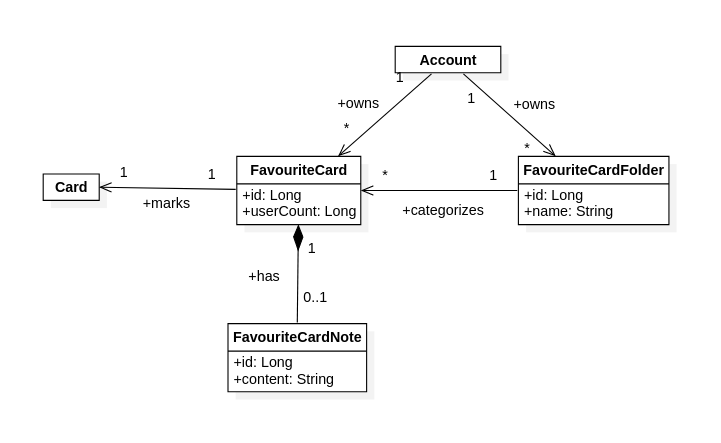
\includegraphics[width=\linewidth]{obrazky/datovy_model_oblibene_karty}\hfill
			\caption{Datový model oblíbených karet uživatelských účtů. Zdroj: [autor]}
		\end{figure}

		Oblíbené karty pak umožňují k uživatelskému účtu přiřazovat cizí karty jako oblíbené pro soukromé uchování a
		poznámkování.
		Každý účet tak může označit libovolný počet karet jako oblíbené, což danému uživateli umožní rychlý přístup
		k požadovaných informacím.
		Každá oblíbená karta může mít navíc jednu textovou poznámku s formátováním pro uživatelské poznámky.
		Oblíbené karty je pak možné seskupovat do složek definovaných uživatelem pro lepší orientaci.
		Složky, poznámky ani oblíbené karty však nevidí nikdo jiný než autor a každý uživatel má tak vlastní sadu těchto dat.

		\subsubsection{Práce s datovým modelem}

		Práci s datovým modelem zastřešuje právě již několikrát zmíněná business logika, která s ním manipuluje k dosažení
		cíle uživatelů.
		Struktura business logiky si bere inspiraci z návrhového vzoru domain-driven design \ac{DDD}, který se zabývá
		navrhováním přehledné, znovu použitelné a hlavně jednoduše rozšiřitelné struktury řešící zadané businessové požadavky
		projektu.
		Tento vzor pohlíží na problematiku jako na doménu problému a staví hlavně na konceptu tzv. služeb,
		což jsou speciální třídy objektového programování, které
		neudržují vnitřní stav, ale poskytují právě služby manipulující s datovými objekty \cite{ddd_quickly}.
		Jednotlivé služby by se měli vždy zabývat pouze jedním typem dat kvůli přehlednosti a ostatní data delegovat na
		ostatní služby \cite{ddd_quickly}.
		Druhým podstatným stavebním blokem jsou repozitáře zajišťující předávání dat mezi aplikací a databázovým systémem
		\cite{ddd_quickly}.
		\ac{DDD} obsahuje spoustu dalších konceptů, nicméně ty byly při implementaci využity jen vzdáleně a ve výsledku
		nereflektují návrhový vzor.
		Implementovaná business logika tak má několik službových tříd a repozitářů.
		Pro každou separátní část modelu existuje manipulující služební třída a jeden repozitář starající se především o
		načítání a ukládání společně s validací do databáze.
		Konzumující logika si pak může vybrat přesně s jakými daty chce pracovat.
		Zatímco repozitáře se starají pouze o komunikaci s databází pomocí \ac{SQL} jazyka nějaké podpůrné knihovny,
		služební třídy tyto informace předávají dál, upravují nebo validují podle potřeb požadavků.

		\begin{figure}[H]
			\centering
			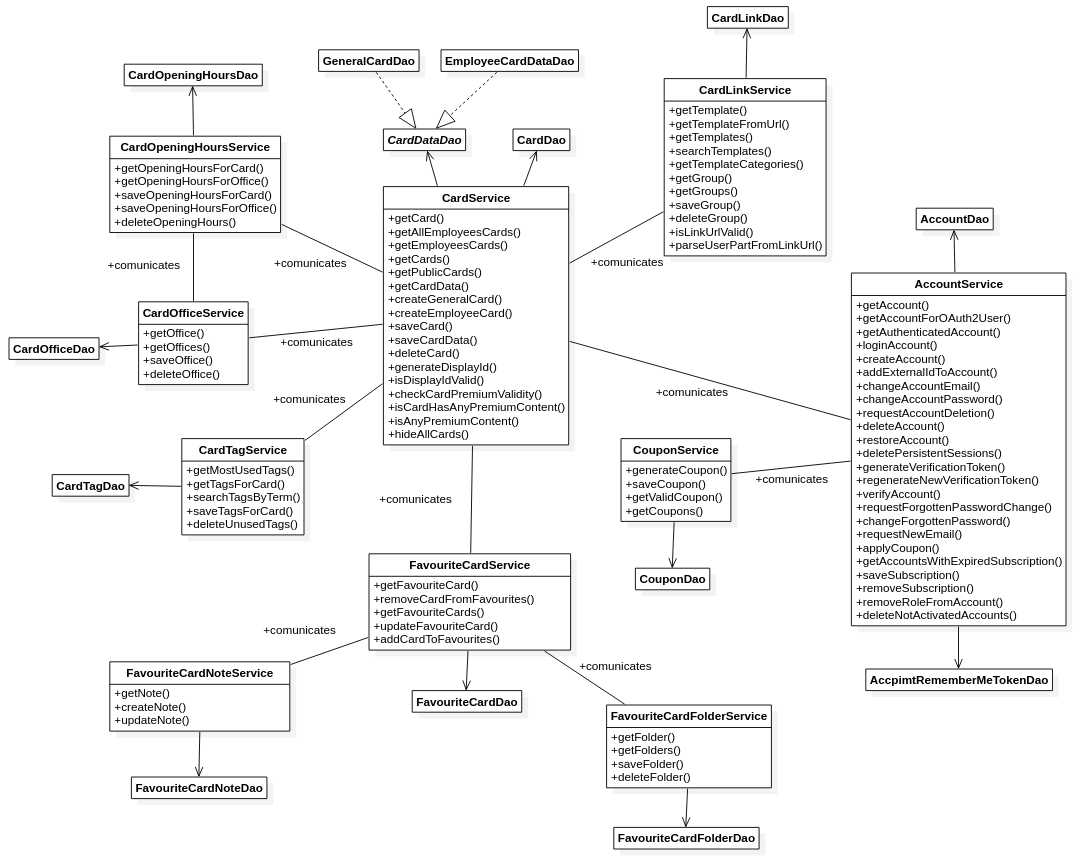
\includegraphics[width=\linewidth]{obrazky/sluzby_a_repozitare}\hfill
			\caption{Zjednodušený model služeb a repozitářů. Zdroj: [autor]}
		\end{figure}

		Momentální implementace služeb komunikuje mezi sebou převážně pomocí primárních klíčů jednotlivých entit, aby
		bylo zaručeno, že entita se kterou služba manipuluje je vždy aktuální verzí reflektující stav databáze.
		Nicméně tento přístup značně zesložiťuje závislost jednotlivých tříd na jiné třídy, což vede k složitějšímu
		instanciování a testování tříd.

		Bohužel, při postupném rozšiřování aplikačních požadavků se ukázalo, že rozpad logických celků entit není při větší
		komplexitě úplně vhodný a i když funguje bez problémů, jeho testování a nastavování už ideální není.
		I pro samotné získání celého logické celku (např.: karta společně se všemi navázanými daty) znamená provolání
		několika služeb a následné ruční sestavení výsledného celku, což vyžaduje zbytečnou vysokou provázanost několika tříd,
		která znemožňuje jednoduché rozšiřování a testování, protože při změně je mnohdy potřeba přepsat podstatnou část
		tříd využívající právě tyto služby.

		Tento problém však řeší právě návrhový vzor \ac{DDD} svými entitami a hodnotovými objekty.
		Podle tohoto vzoru by se mělo pracovat s logickými celky jako s jednou entitou, aby se předešlo výše zmíněné složitosti
		rozpadlosti služebních tříd.
		Další podstatnou výhodou této provázanosti je zaručení konzistentnosti dílčích entit.
		Tento problém implementovaný přístup řeší také, a to pomocí validací, nicméně složitost opět rapidně stoupá kvůli
		nutnosti stále se dotazovat na stav nadřazených entit na více místech.
		\cite{ddd_quickly}
		Pro momentální stav aplikace implementovaný model je dostačující, nicméně pro budoucí rozšíření by bylo nutné
		model značně optimalizovat za pomocí \ac{DDD} vzorů, které se sice nedají vždy aplikovat na každý problém, avšak
		ve většině případů tyto vzory pomáhají zpřehlednit model (záleží ale také na konkrétní implementaci vzorů).

		\subsubsection{Komunikace s databázových systémem}

		Prvním problémem k řešení při implementaci již samotné business logiky třídách služeb a repozitářů je výběr
		přístupu mapování objektů do databázové struktury.

		V případě, že by aplikace využívala nějakou z \ac{NoSQL} databází s podporou \ac{JSON} dokumentů, bylo by toto
		mapování poměrně jednoduché.
		Jedinou složitost by pravděpodobně představovalo mapování hierarchických karet, protože například MongoDB pouze
		značně omezené propojování mezi jednotlivými kolekcemi.

		V případě vybrané \ac{SQL} databáze je ale problém složitější, protože tyto databáze pracují s tabulkami místo objekty.
		Na první pohled se může zdát, že by to neměl být velký problém, protože sloupce tabulek jsou podobné vlastnostem
		objektům a \ac{SQL} databáze jsou dělané pro propojování navzájem čehokoliv.
		Bohužel problém spočívá právě v překladu mezi relačním modelem a objekty.
		Složitost je hlavně v načítání a ukládání komplexních složených entity z více objektů a kolekcí, hlavně pak
		kolekcí 1:N.
		Jazyk \ac{SQL} totiž neumožňuje jednoduše vrátit více řádků z jiných tabulek a tak není možné najednou
		vrátit objekty jiných tříd, kde jedna třída se mapuje na jednu tabulku.
		Stejný problém je i v případě ukládání dat, protože \ac{SQL} umožňuje ukládání pouze řádků do jedné tabulky.
		Horší to je ještě v případě ukládání již existujících dat, kdy \ac{SQL} neumožňuje hromadné úpravy.

		Naštěstí existuje několik knihoven a nástrojů pro, které tyto problémy více či méne řeší za programátora.
		Je možné vše implementovat ručně pomocí knihoven, které pouze zastřešují \ac{SQL} komunikaci a už neřeší
		právě to mapování.
		Nicméně kromě hodně specifických projektů, je tento přístup zbytečně složitý (zvýšený čas a nepřehledný kód)
		a knihovny navíc mnohdy tyto problémy řeší efektivněji.
		Mezi nejpoužívanější knihovny patří Hibernate a MyBatis.
		Poměrně novou zajímavou alternativou je Spring Data JDBC, bohužel tato knihovna v době vývoje nebyla příliš
		rozšířená a neosvědčená.

		Hibernate a MyBatis mají dost rozdílné přístupy k řešení výše zmíněných problémů.
		Zatím co Hibernate se snaží být plným \ac{ORM} frameworkem a odstínit programátora pokud možno od jakéhokoliv
		\ac{SQL} jazyka \cite{hibernate_docs}, MyBatis je lehčí alternativa, která poskytuje spíše nástroje pro mapování a dotazování, ale
		nezatěžuje programátora všemi nízkoúrovňovými problémy \cite{mybatis_getting_started}.
		Další velký rozdíl jakým knihovny pracují s entitami na pozadí.
		Hibernate využívá mezičlánku mezi repozitářem a databází, kde jsou dočasně entity uloženy \cite{hibernate_docs}.
		Díky tomu je Hibernate schopen poskytovat mezipamět pro entity při vícenásobném stahování a při ukládání
		se data nepromítají hned ale až na konci transakce \cite{hibernate_docs}.
		Kvůli tomu se tak repozitář chová spíše jako paměťové úložiště, kde má programátor okamžitý přístup k objektům.
		Bohužel to má i svá úskalí a to nejen v celkové komplexitě knihovny kvůli vysoké abstraktnosti, která může navíc
		i přístup k datům do jisté míry zpomalovat, právě díky té abstraktnosti.
		Úskalí se skrývá, hlavně pro tento projekt, v sdílení instancí reprezentujících jednu entitu při vícenásobném
		dotažení entity z databáze.
		Tento přístup zamezuje porovnávání originální verze entity a nové upravené (většinou přijaté skrze \ac{API} k
		uložení), protože interně ji Hibernate považuje za jednu instanci.
		Hibernate sice má dobré nástroje pro validaci dat entit, ty však validují pouze aktuální hodnoty v objektu a
		není možné porovnat hodnoty z již uloženou entitou v databázi.
		To je v případě kdy má vlastnosti, které se nesmí změnit poměrně limitující.
		Instance entity sice lze vyjmout z Hibernatu, je to však poměrně složité a těžkopádné a tím se zesložiťuje
		celá business logika.
		MyBatis tento neduh nemá a vrací vždy novou instanci entity.
		MyBatis se obecně nesnaží řešit vše a díky tomu jeho abstrakce je mnohem menší a snazší na pochopení.
		To ovšem znamená, že programátor musí odvést více práce při mapování a psát \ac{SQL} dotazy.
		Musí také ručně řešit ukládání složených entit, což Hibernate na proti tomu řeší.

		I když by se mohlo zdát, že Hibernate je ultimátním nástrojem pro 99\% projektů, existuje mnoho materiálů
		zkušených programátorů využívajících Hibernate spoustu let, kteří si nemyslí, že Hibernate je ideálním nástrojem.
		Jeho komplexnost abstrakce totiž může přinést spoustu problémů, které na první pohled nemusí někoho napadnout.
		Mezi největší problémy patří nejednoznačné chyby mapování, nutnost přizpůsobit databázový model zvyklostem Hibernatu
		(který nesplňuje běžné doporučované postupy), náhodné chyby s dodatečným dotahováním dat nebo nejednoznačné operace
		v \ac{API} knihovny.
		Na druhou stranu spousta uživatelů této knihovny jsou spokojeni s odstíněním \ac{SQL} jazyka a problémů jako
		mapování kolekcí a podobně. \cite{bad_hibernate}

		Záleží tedy hodně na konkrétním projektu a zkušenostech implementátorů jakou knihovnu zvolit.
		Pro tuto aplikaci byl z počátku zvolen Hibernate právě díky jeho odstínění od problémů mapování a poměrně
		jednoduché konfigurace složitějších entit.
		Bohužel se posléze začal projevovat již zmiňovaný problém validací verzí entit.
		Po dodatečné analýze padlo rozhodnutí nahradit Hibernate MyBatisem.
		Za cenu prvotní transformace, MyBatis zjednodušil práci s entitami a hledání chyb bylo přímočařejší.
		MyBatis navíc podporuje konfiguraci pomocí \ac{XML} souborů nebo pomocí Java anotací přívo v Java rozhraních.
		Pro zjednodušení a držení logiky na jednom místě byl vybrán přístup s Java anotacemi.
		Ten se ukázal jako dostačující ve většině případů, avšak výjimky se našli, kdy složitost použitého \ac{SQL} kódu
		byla na hraně přehlednosti v rámci Java rozhraních.
		Momentálně tedy existuje pro každý typ entity třída reprezentující repozitář obsahující metody obalené \ac{SQL}
		dotazy definující chování metody.
		Na základě definovaných metod a \ac{SQL} kódu pak MyBatis dynamicky vygeneruje konkrétní třídy zajišťující tuto
		logiku.
		Zde je možné vidět reprezentativní ukázku části repozitáře pro práci uživatelskými účty.

		\begin{lstlisting}[language=Java,caption={My Caption}]
@Mapper
public interface AccountDao {
	@Select({
		"select *",
		"from " + Account.TABLE_NAME,
		"where email = #{email}"
	})
	Optional<Account> findByEmail(String email);
}
		\end{lstlisting}

		% todo
 		Získání uživatelského účtu z databáze společně s vnořeným předplatným a kolekcí rolí.
		Entita je pak automaticky namapována MyBatisem díky stejnému pojmenování sloupců tabulek a atributů třídy.

		\subsubsection{Validace entit}

		Validace entit je velice důležitá, pokud uživatelé mohou data upravovat zvenčí.
		Díky ní se do databáze dostanou jen validní data.
		Tato aplikace využívá dva typy validace, každou pro validování něčeho jiného.
		První a hlavní validací je běžně využívaná validace formátu hodnot v entitách.
		Tato validace je ta jednodušší protože je jasně předem daný formát hodnot a navíc existují knihovny, které
		značně zjednodušují práci.
		Co se týče formátu hodnot, tím může být ku příkladu maximální délka textového řetězce, omezení pouze na velká
		písmena nebo maximální číselná hodnota.
		Druhým typem využívané validace v implementované aplikaci je validace, že určité hodnoty se u upravených entit
		nezměnily oproti původní verzi.
		Takovými hodnotami jsou většinou stavy entity nebo různé datumy.
		Příkladem může být stav karty, kdy smazaný karta již nesmí přejít do stavu aktivní karty, protože nemá potřebná data.
		Dalším příkladem je datum vytvoření entity, který se nesmí změnit jinak by postrádal svůj účel nebo typ karty,
		protože systém nepodporuje změnu typu karty (technicky náročné, protože každý typ karty obsahuje úplně jiný data
		a má jiný účel).

		Pro tento projekt byla využita knihovna Hibernate Validator zabývající se především prvním typem validací
		využívající Java anotace pro specifikování jednotlivých pravidel.
		Pravidla se můžou stahovat buď na celou třídu nebo na konkrétní atributy třídy.
		Knihovna sama o sobě poskytuje rozsáhlou sadu běžných pravidel, avšak umožňuje jednoduché implementování vlastních
		pravidel.
		Takto může vypadat třída s definovanými pravidly.
		\begin{lstlisting}[language=Java]
@CardLinkUrl
public class CardLinkGroup {

	@CardLinkTemplateId
	private String templateId;

	@NotNull
	@Size(min = 1)
	private List<@Valid CardLink> links;
}
		\end{lstlisting}
		Tato třída obsahuje vlastní třídní pravidlo pro validaci \ac{URL} adres vnořených odkazů na základě definované šablony,
		atributové pravidlo pro validaci existence šablony a validaci kolekce odkazů, která nesmí být prázdná.

		Díky rozšířitelnosti této knihovny je možné poměrně jednoduše implementovat i druhý typ validací.
		Tyto validace pak mají vlastní Java anotace tvářící se jako běžná pravidla, mají však vlastní implementaci
		validátoru ověřující validovaný objekt.
		Zde je vidět ukázka validátoru ověřující neměnitelné atributy upravené karty oproti její původní verzi:

		\begin{lstlisting}[language=Java]
public class UpdatedCardValidator implements ConstraintValidator<UpdatedCard, Card> {
	@Override
	public boolean isValid(Card updatedCard, ConstraintValidatorContext context) {
		final Optional<Card> originalCard = cardService.getCard(updatedCard.getId(), true);
		/* ... */
		if (originalCard.get().getState().equals(CardState.DELETED)) {
			return false;
		}
		if (!updatedCard.getType().equals(originalCard.get().getType())) {
			return false;
		}
		/* ... */
		return true;
	}
}
		\end{lstlisting}

		Pokud se nějaký takový atribut změnil o proti původní verzi změnil, validace selže a neumožní uživateli
		uložit novou verzi entity.

		Po nastavení pravidel entitám je již možné provádět samotnou validaci.
		K tomu v knihovně Hibernate Validator slouží jedna centrální třída reprezentující validátor příjímající
		entitu označenou pravidly a vrací kolekcí nalezených porušení pravidel.
		Je pak už na programátorovi jak s touto kolekcí naloží.
		V případě této aplikace, kód vyhodí výjimkou, která se následně v \ac{API} přeloží na chybu.
		\begin{lstlisting}[language=Java]
final Set<ConstraintViolation<Card>> violations = validator.validate(updatedCard);
Assert.isTrue(
		violations.isEmpty(),
		"Card is not valid: " + violations.stream().map(ConstraintViolation::getMessage).collect(Collectors.joining("; "))
);
		\end{lstlisting}

		\subsubsection{Úložiště souborů}

		Jak již bylo nastíněno, aplikace nebude implementovat vlastní souborové úložiště s generováním variant obrázků.
		Místo toho bude využívat externí službu Cloudinary, která zajistí uchování souborů, generování variant obrázků
		a \ac{CDN} pomocí \ac{REST} \ac{API} zajišťující komunikaci mezi aplikací a službou.
		Cloudinary navíc poskytuje knihovnu obalující \ac{REST} \ac{API} přímo do Java tříd, takže se není potřeba zabývat
		komunikací čistým \ac{REST} \ac{API}.
		Aplikace bude \ac{API} využívat k ukládání souborů a získávání uložených souborů pro interní validace.
		Získávání variant obrázku do \ac{GUI} bude zajišťovat přímo front-endová aplikace.

		Cloudinary poskytuje jeden velký adresář pro všechny soubory, což je při více typů souborů nevhodné.
		Naštěstí podporuje vnořené adresáře.
		Právě kvůli tomu vznikl koncept předem definovaných tzv. typů uložišť, kde každý typ definuje cestu
		relativního kořenového adresáře, typ ukládaných souborů a interní ID.
		Momentálně existuje pouze jedno uložiště a to pro profilové obrázky karet

		\begin{lstlisting}[language=Java]
public enum StorageType {
    CARDS_AVATARS("cards-avatars", "cards/avatars", "image");

    private final String id;
    private final String folderPath;
    private final String resourceType;
}
		\end{lstlisting}
		Ukázka definových typů uložišť. % todo

		Aby bylo možné zpětně jednoduše identifikovat autora a typ uložiště uloženého souboru, je potřeba ke každému
		souboru definovat dodatečná metadata.
		Cloudinary naštěstí takový metadata podporuje.
		Každý uložený soubor je pak popsán následující třídou obsahující všechny potřebné informace o souboru pro zobrazení
		a validaci:

		\begin{lstlisting}[language=Java]
public class StorageFile {
    private final StorageType storageType;
    private final long ownerId;
    private final String publicId;
    private final String url;
}
		\end{lstlisting}

		% todo popis
		ID uživatelského účtu, který tento soubor nahrál
		ID soubor v Cloudinary uložišti
		veřejná URL adresa, na které je obrázek možné zobrazit

		Autor a typ úložiště slouží momentálně hlavně k jednoduché validaci zvoleného obrázku při ukládání karty, kdy
		se validuje jestli majitel karty je zároveň majitelem obrázku a zda-li se jedná skutečně o profilový obrázek.
		Tyto validace existují, aby nebylo možné někým záměrně využít obrázek někoho jiného nebo soubor, který k tomu
		není určený.

		Finální uložení se pak už skládá pouze z načtení binárních dat obrázku a sestavení výše zmíněných metadat a zavolání \ac{API}
		služby:

		\begin{lstlisting}[language=Java]
final long authenticatedAccountId = accountService.getAuthenticatedAccount().getId();
final Map<String, Object> params = buildFileUploadParams(storageType, authenticatedAccountId);

final BufferedInputStream bis = new BufferedInputStream(file.getInputStream());
final byte[] fileBytes = bis.readAllBytes();

cloudinary.uploader().upload(fileBytes, params);
		\end{lstlisting}

		% todo
		sestavení metadat
		načtení souboru
		nahrání souboru do Cloudinary

		Získání popisného souboru z Cloudinary je podobně jednoduché jako uložení.
		\ac{API} umožňuje získat data o jednotlivých souborech pomocí interního ID a požadavek lze obohatit o dodatečné požadavky.
		V případě této aplikace se výsledek obohacuje o metadata.

		\begin{lstlisting}[language=Java]
final Map<String, Object> params = new HashMap<>();
params.put("metadata", true);

final ApiResponse response = cloudinary.api().resource(publicId, params);

return Optional.of(new StorageFile(
	StorageType.getById((String) ((Map) response.get("metadata")).get(STORAGE_FILE_METADATA_STORAGE_TYPE_NAME)),
	((Integer) ((Map) response.get("metadata")).get(STORAGE_FILE_METADATA_OWNER_ID_NAME)).longValue(),
	(String) response.get("public_id"),
	(String) response.get("secure_url")
));
		\end{lstlisting}

		Popisující soubor obecně používá na místech, kde nejsou potřeba konkrétní binární data souboru, ale pouze
		informace o něm.
		Binární data jsou většinou potřeba pouze v případě zobrazení souborů v \ac{GUI} nikoliv přímo v aplikaci díky
		odstínění generování variant.

		Konkrétní binární data souborů pro zobrazení například v \ac{GUI} aplikace je možné získat přímo ze serverů
		Cloudinary pomocí speciální \ac{URL} adresy obsahující identifikaci úložiště, identifikaci konkrétního souboru a
		požadovanou variantu.
		Díky přímému přístupu je možné využít \ac{CDN} pro menší odezvy při stahování.
		Konkrétní \ac{URL} adresa pro stažení profilové obrázku karty v podobě varianty o rozměrech 256x256 pixelů může
		vypadat následovně:
		\begin{lstlisting}
https://res.cloudinary.com/id_uloziste/image/upload/t_256x256/id_souboru
		\end{lstlisting}
		V tomto případě je varianta nakonfigurována přímo v administraci Cloudinary a v \ac{URL} adrese je pouze její jméno,
		je však možné formát varianty nadefinovat přímo v \ac{URL} adrese.

		\subsubsection{Transakční emaily}

		Aby bylo možné upozorňovat uživatele na nečekané údalosti vzniklé v aplikaci nebo zaslání informací uživateli,
		je potřeba nějaký komunikační kanál.
		Jak již bylo zmíněno, tím budou emailové zprávy.
		Cílem je tedy vytvořit systém odesílající předem definované zprávy přiřazené konkrétním událostem.
		Stejně jako v případě souborového úložiště, aplikace nebude implementovat vlastní řešení, ale využije externích
		služeb.
		Vlastní řešení by znamenalo značnou zátěž na implementaci aplikace a i tak by bylo nutné napojit odesílání
		emailů na ověřeného odesílatele emailů, aby emaily nekončily uživatelům v nevyžádané poště.
		Proto bylo zvoleno využít externí službu SendinBlue, která poskytne vše potřebné již připravené skrz \ac{API}
		s existující Java knihovnou.
		V aplikaci už je pak nutné pouze připravit propojení mezi tímto \ac{API} a událostmi v aplikaci.

		Pro odesílaní emailů je nejdříve nutné připravit šablony zpráv, aby bylo co odesílat.
		Ty lze připravit buď ručně pomocí šablonovacího jazyk (např.: FreeMarker) a odeslat pomocí \ac{API} do externí
		služby nebo v případě SendinBlue lze využít integrovaného klikacího editoru umožňujícího jednoduše připravit
		šablony pomocí předpřipravených prvků.
		Obsah emailů se vytváří v jazyce \ac{HTML}, nicméně podpora zobrazování ostylovaného \ac{HTML} obsahu v
		emailových klientech je poměrně omezená a velice se liší mezi jednotlivými klienty.
		Kvůli tomu je časově náročné připravit šablonu fungující na všech populárních klientech a to navíc ve dvouch
		verzích: desktopové a mobilní.
		Tyto problémy do jisté míry řeší právě interaktivní editor, avšak za cenu nižších možností přizpůsobení vzhledu
		a struktury.
		Výhodou je, že SendinBlue poskytuje oba přístupy a není problém použít jeden nebo druhý.
		Právě proto padla volba na interaktivní editor, který ušetří v začátku spoustu času a v budoucnu je možné
		přejít na vlastní šablony.

		Každá šablona má v systému unikátní ID, takže byla tvořena jednoduchá enumerace pro explicitní mapování
		šablon ke kryptickým identifikátorům.

		\begin{lstlisting}[language=Java]
public enum EmailTemplate {
    NEW_ACCOUNT_CONFIRMATION(1),
    NEW_ACCOUNT_WELCOMING(2),
    ACCOUNT_PASSWORD_CHANGED(3),
    ACCOUNT_FORGOTTEN_PASSWORD(4),
    ACCOUNT_NEW_EMAIL(5),
    ACCOUNT_EMAIL_CHANGED(6),
    ACCOUNT_DELETED(7),
    ACCOUNT_SUBSCRIPTION_WILL_EXPIRE(8),
    ACCOUNT_SUBSCRIPTION_EXPIRED(9),
    ACCOUNT_SUBSCRIPTION_EXPIRATION_WARNING(10),
    ACCOUNT_SUBSCRIPTION_EXPIRATION_FINAL_ACTION(11);

    private final long id;
}
		\end{lstlisting}

		Díky této enumeraci je pak v aplikaci jasné jaká šablona bude použita.
		Dále může šablona využívat parametry místo konkrétního textu, které jsou při zpracování šablony nahrazeny
		parametry požadavku.
		Těmi může být cokoliv, například emailová adresa adresáta nebo expirační datum nějaké entity.

		Odeslání konkrétního emailu už je pak jednoduché a vyžaduje pouze specifikování emailové adresy adresáta,
		šablonu emailu a volitelně i parametry šablony.
		Aplikace pak už pouze sestaví požadavek o odeslání emailu a předá ho \ac{API}.

		\begin{lstlisting}[language=Java]
public CreateSmtpEmail sendTransactionalEmail(@NonNull String to, @NonNull EmailTemplate template, Properties templateArguments) {
	final SendSmtpEmail sendSmtpEmail = new SendSmtpEmail();

	final SendSmtpEmailTo sendSmtpEmailTo = new SendSmtpEmailTo();
	sendSmtpEmailTo.email(to);
	sendSmtpEmail.to(List.of(sendSmtpEmailTo));

	sendSmtpEmail.setTemplateId(template.getId());

	if (templateArguments == null) {
		templateArguments = new Properties();
	}
	templateArguments.put(DOMAIN_TEMPLATE_PROPERTY_NAME, appConfig.getDomain());
	sendSmtpEmail.setParams(templateArguments);

	try {
		log.info("Sending transaction email to " + to + " with template " + template + " ...");
		return new TransactionalEmailsApi(apiClient).sendTransacEmail(sendSmtpEmail);
	} catch (ApiException e) {
		throw new RuntimeException("Could not send transactional email to " + to + " with template " + template + ": ", e);
	}
}
		\end{lstlisting}

		Jak bylo nastíněno, systém bude odesílat emaily automaticky jako reakci na vzniklé události v aplikaci.
		Události jsou v tomto případě reprezentování aplikačními událostmi z frameworku Spring.
		Spring umožňuje do systému publikovat aplikační události a definovat pozorovatele, kteří naslouchají na konkrétní
		vzniklé aplikační události a mohou na ně reagovat vykonáním libovolných operací.
		Samotná aplikační událost je pouze jednoduchý objekt nesoucí kontextové data reprezentovaná událostí.

		\begin{lstlisting}[language=Java]
public class CardUpdatedEvent extends ApplicationEvent {
    private final Card originalCard;
    private final Card updatedCard;

    /* ... */
}
		\end{lstlisting}

		Příkladem může být událost vyvolaná jako následek uložení upravené karty.
		Událost tedy reprezentuje úpravu karty a může sebou nést danou upravnou kartu, kterou pozorovatel může
		využít pro provedení svých operací.
		\begin{lstlisting}[language=Java]
public class CardUpdatedEventListener {
    @EventListener
    public void processCardUpdatedEvent(@NonNull CardUpdatedEvent event) {
        /* ... */
    }
}
		\end{lstlisting}

		Právě tento přístup využívá modul odesílání emailů.
		Modul má do systému vystavené vlastní posluchače na konkrétní aplikační události (změna emailu uživatele, změna hesla,
		vypršení platnosti předplatného...) vytvářející požadavky pro odesílání správných emailů.
		Tento přístup vhodný, protože moduly uživatelských účtů, karet a podobně vůbec nevědí o modulu emailů a nevzniká
		tak fyzické propojení znepřehledňující kód.
		Navíc je pomocí aplikačních události jednoduché přidávat nové události a jejich posluchače.

		\begin{lstlisting}[language=Java]
@EventListener
public void processAccountNewEmailRequestedEvent(@NonNull AccountNewEmailRequestedEvent event) {
	final Properties templateArguments = new Properties();
	templateArguments.put(TOKEN_TEMPLATE_PROPERTY_NAME, event.getVerificationToken().getToken());
	mailService.sendTransactionalEmail(event.getNewEmail(), EmailTemplate.ACCOUNT_NEW_EMAIL, templateArguments);
}
		\end{lstlisting}
		Ukázka odeslání emailu jako reakce na událost informující o novém požadavku na změnu hesla. % todo

		\subsubsection{Vyhledávání karet a míst}

		Fulltextové vyhledávání je komplexní operace, který vyžaduje analýzu textů a přípravu vyhledatelných dat.
		Tyto data musí být při vyhledávání korektně párována s uživatelkou frází, tak aby systém vrátil co nejrelevantnější
		výsledky.
		Naštěstí existují nástroje zabývající se touto problematikou.
		Vybraným nástrojem pro tuto aplikaci je populární a všestranný databázový systém Elasticsearch.
		Ten umí spoustu věcí, avšak pro tento projekt je důležitá problematika fulltextového vyhledávání.
		Tuto problematiku Elasticsearch schovává před programátorem a programátorovi stačí pouze popsat
		vyhledatelné entity a při vyhledávání definovat pouze požadavky.

		I přes míru abstrakce je potřeba znát základní koncepty fulltextového vyhledávání.
		Fulltextové vyhledávání pracuje s tzv. analyzátory, kteří analyzují text a generují z něj index relevantních
		slov podle určených pravidel.
		Tento proces je aplikovat na vyhledatelné dokumenty i na vyhledávací frázi zadanou uživatelem.
		Vygenerované indexy se při vyhledávání porovnávají a podle určitých kritérií, databáze vyhodnotí relevantnost
		dokumentu pro vyhledávanou frázi. \cite{index_search_analysis}

		Každý analyzér se skládá z filtrů znaků, tokenizérů a filtrů tokenů.
		Filtry znaků v analyzovaném textu upravují jednotlivé znaky.
		Znaky mohou přidávat, odebírat nebo nahrazovat jinými (např.: odstranění diakritiky).
		Poté je takto upravený text předán tokenizérům, kteří text rozdělí na kolekci tokenů.
		Token může představovat cokoliv co dává v kontextu aplikace smysl, nicméně většinou token přestavuje jedno
		slovo věty.
		Tyto tokeny můžou být ještě upraveny pomocí filtrů tokenů.
		Ty podobně jako filtry znaků umožňují přidávání, úpravu a mazání tokenů.
		Těmi mohou být: filtr pro odmazání generických slov bez přidaného významu (např.: spojky), filtr pro odstranění
		diakritiky nebo filtr pro převedení tokenů na malá písmena, aby nezáleželo na tvaru zadaného slova oproti slovu
		v dokumentu.
		Výsledné tokeny pak tvoří index, nad kterým lze již vyhledávat.
		\cite{analyzer_anatomy}

		Elasticsearch pracuje s tzv. indexy, což jsou kolekce indexovaných \ac{JSON} dokumentů entit stejného typu.
		Tyto dokumenty pak lze vyhledávat pomocí dotazovacího jazyka.
		Každý index má kromě samotných dat i konfiguraci jak s daty pracovat.
		Kromě obecných konfiguračních hodnot obsahuje hlavně strukturu dokumentů, aby databáze mohla efektivně vyhledávat
		nad uloženými daty.
		Tato definice zahrnuje v první řadě určení datových typů jednotlivých hodnot entit.
		Od datového typu se pak odvíjí další dostupné konfigurační hodnoty.
		Nejdůležitějším takovým nastavením pro fulltextové vyhledávání je specifikování analyzérů pro textové hodnoty.
		Specifikované analyzéry by měli odpovídat analyzéru použitému při vyhledávání pro kompatibilitu indexů tokenů.

		Elasticsearch pro práci s těmito indexy a dokumenty poskytuje Java knihovnu reflektující jeho \ac{REST} \ac{API},
		prostřednictvím které lze jednoduše nahrávat entity do indexu k indexaci.

		\begin{lstlisting}[language=Java]
final SearchableCard cardToIndex = searchableCardFactory.create(card);
final IndexResponse cardResponse = esClient.index(i -> i
		.index(SearchableCard.INDEX_ALIAS)
		.id(String.valueOf(card.getId()))
		.document(cardToIndex));
		\end{lstlisting}
		Ukázka indexace jedné karty do Elasticsearch databáze. % todo

		% todo
		vytvoření entity
		nahrání entity do Elasticsearch indexu, který ji automaticky zanalyzuje

		Podobně jednoduše lze entity fulltextově vyhledávat napříč vícero atributy entit
		\begin{lstlisting}[language=Java]
final SearchResponse<SearchableCard> response = esClient.search(
		_0 -> _0
				.index(SearchableCard.INDEX_ALIAS)
				.query(_1 -> _1
					.multiMatch(_2 -> _2
						.query(phrase)
						.analyzer(ANALYZER_MAIN)
						.fields(
							"name",
							"description",
							"contactEmail",
							"contactPhone",
							"jobPosition",
							"crn",
							"website",
							"linkProfiles",
							"tags")))
				.from(pageSpecs != PageSpecs.UNPAGED ? (int) pageSpecs.getOffset() : null)
				.size(pageSpecs != PageSpecs.UNPAGED ? (int) pageSpecs.getSize() : null),
		SearchableCard.class);
		\end{lstlisting}

		Hlavní řešený problémy tak spočívají spíše v v přípravě entit a správě indexů a jejich konfigurace.
		Tuto problematiku totiž Elasticsearch knihovna řeší ve formě dílčích operací, nikoliv však jako celek.
		Bylo potřeba vyřešit indexaci a vyhledávání karet a geografických míst.
		Karty musí být uživatel schopen vyhledat fulltextově skrze vícero atributů (název, popisek, odkazy...) a geografická
		místa podle lokace uživatele.

		První jednodušší problematikou je příprava entit.
		Mohlo by se zdát, že tento problém nastane spíše v nestandardním projektu, avšak data využívaná k vyhledávání
		jsou trochu jiná než ta hlavní.
		V případě karet je nebytné komplexní strukturu všech navázaných dat značně zjednodušit, proto by jinak Elasticsearch
		nebyl schopen tolik zanořená data správně analyzovat.
		Některé atributy je zase potřeba zagregovat do jiné formy.
		V případě geografických míst je na proti tomu nutné zagregovat více různých dat a paradoxně struktury míst lehce
		zesložitit, aby obsahovala vše co uživatel potřebuje.

		\begin{lstlisting}[language=Java,label{lst=Ukázka indexovatelné varianty karty.}]
public class SearchableCard {

    String displayId;
    String avatarId;
    Set<CardLinkDto> links;
    CardOpeningHoursDto openingHours;

    String name;
    String website;
    String contactEmail;
    String contactPhone;
    String description;
    String crn;
    String jobPosition;
    Set<String> linkProfiles;
    Set<String> tags;
    Set<String> officeNames;

    /* ... */
}
		\end{lstlisting}

% todo
metadata pouze pro následné zobrazení entity
atributy, podle kterých lze fulltextově vyhledávat

		Na ukázce varianty karty připravené pro indexaci je možné vidět právě zmiňované zjednodušení a agregace dat.
		První řadě třída obsahuje pouze část originálních dat, která jsou relevantní pro vyhledávání.
		Následně je možné vidět, že karta obsahuje data z různých typů karet nebo jen části vnořených entit (z poboček jsou
		zde pouze jejich názvy).

		Ukázkovým příkladem agregace je pak kolekce profilových ID odkazů.
		Originální karta má totiž přístup pouze k cílovým \ac{URL} adresám odkazům a je tak na aplikaci, aby z těchto dat
		vytáhla ID profilů uživatelů.
		K tomu využívá šablony \ac{URL} adres z šablon sítí a standardizovaného formátu \ac{URL} adres.
		Pomocí \ac{URL} šablony je možné získat část \ac{URL} adresy, která je specifická pro uživatele a obsahuje profilové ID.
		Tento řetězec je následně očištěn částí \ac{URL} adres jako jsou: část cesty nebo dotazovací parametry.

		\begin{lstlisting}[label={lst=Ukázka transformace URL adresy na profilové ID.}]
// URL adresa
https://example.com/profile/jan_novak?detail
// ID
jan_novak
		\end{lstlisting}

		Tyto transformovací operace zajišťují speciální třídy tzv. továrny, které vezmou originální entity a vytvoří
		z ní indexovatelnou entitu.
		Takové entity již lze předat \ac{API} k indexaci.

		Dalším složitějším problémem je změna struktury dat a změna konfigurace již existujících indexů.
		Je předpokládatelné, že entity se v průběhu vývoje budou měnit a rozšiřovat.
		Bohužel tím že Elasticsearch je spíše vyhledávacím strojem než klasickou databází, neposkytuje nástroje pro editaci
		dílčích data již indexovaných entit jako tomu je v případě \ac{SQL}.
		Stejně tak má omezené nástroje pro úpravu konfigurace indexu a není proto možné jednoduše změnit například
		použitý analyzátor.
		Naštěstí Elasticsearch nabízí alespoň možnost vzít dokumenty z jednoho indexu a zindexovat je do jiného pomocí jeho
		konfigurace.
		To ovšem stále neřeší stav kdy se změnila struktura entit nebo formát jednotlivých atributů entit.
		Bylo proto nezbytné vytvořit systém správy těchto dat, který by zajistil reindexaci všech entit dvěma způsoby.
		Oba způsoby mají podobnou základní strukturu, ale liší se v samotné přípravě dat.
		Proces nejdřív vytvoří nový prázdný index s novým nastavením.
		Následně se některým ze způsobů indexují data do nového indexu.
		Po dokončené indexaci je možné přesunout unifikovaný identifikátor indexu na nový index a starý index premanentně
		smazat.

		Prvním jednodušším a rychlejším způsobem je reindexace na úrovni Elasticsearch.
		Pro tento případ má Elasticsearch připravené jednoduché \ac{API}, kde programátor pouze specifikuje starý a nový
		index a vše ostatní už si zařídí sám Elasticsearch.
		Tento způsob však nenabízí možnost nahrání upravených dat entit, pouze změnu konfigurace indexu.

		\begin{figure}[H]
			\centering
			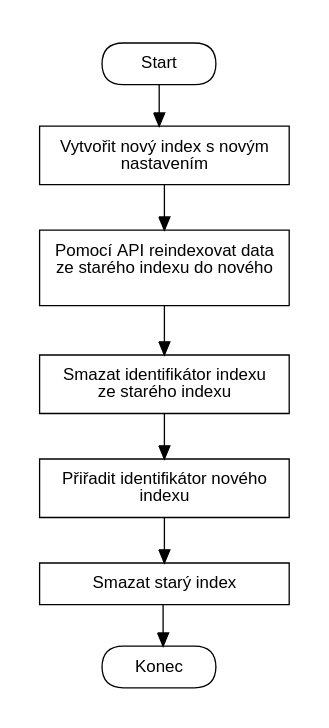
\includegraphics[width=5cm]{obrazky/proces_reindexace_na_urovni_es}\hfill
			\caption{Ukázka procesu hromadné reindexace dat na úrovni Elasticsearch. Zdroj: [autor]}
		\end{figure}

		Druhým složitějším a časově náročnějším způsobem, který však umožňuje indexovat kompletně nová data, je
		reindexace dat z primární databáze.
		Tento způsob vyžaduje hromadné stažený entit z primární databáze, jejich transformaci do indexovatelných entit
		a konečně hromadnou indexaci pomocí \ac{API}.
		Tento proces je zdlouhavý právě kvůli nutnosti přesunutí dat mezi dvě kompletně oddělenými systémy přes mezičlánek,
		kterým je aplikace.

		\begin{figure}[H]
			\centering
			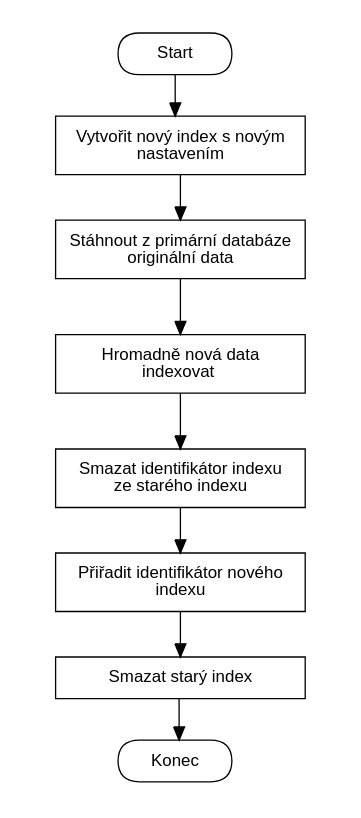
\includegraphics[width=5cm]{obrazky/proces_reindexace_z_db}\hfill
			\caption{Ukázka procesu hromadné reindexace nových dat z primární databáze. Zdroj: [autor]}
		\end{figure}

		Každý index pak má svého správce obsahující napojení na korektní index a jeho nastavení, aby se nastavení nemohla
		mezi indexy míchat.

		\subsubsection{Nastavení aplikace}

		Nedílnou součástí větší aplikace běžící ve více prostředích jsou rozdílná nastavená na každém takovém prostředí.
		Nastavení každé aplikace je vysoce individuální a záleží čistě na požadavckých aplikace jaké nastavení potřebuje
		se změnou prostředí změnit.
		U většiny aplikací se nachází alespoň nastavení připojení k primární databázi, která je pro každého prostředí
		odlišná, aby nedocházelo k poškození dat (např.: mezi vývojovým a produkčním prostředím).
		Dalšími otázkami jsou formát zápisu nastavení a přístup k nastavení z kódu aplikace.
		V případě Java aplikací se často využívá tzv. "properties" souborů obsahující nastavení v podobě klíč-hodnota.
		V modernějších aplikacích postavených na frameworku Spring se ale tento formát postupně nahrazuje flexibilnějším
		\ac{YAML} umožňující lépe definovat celé objekty a hodnoty jejich atributů podobně jako jazyk \ac{JSON}.

		\begin{lstlisting}
accounts:
	deletion:
		process-accounts-deletion-requests-every: 300
		delete-account-after: 180
	subscription:
		process-expiration-every: 60
		\end{lstlisting}
		Ukázka části nastavení aplikace v jazyce YAML. % todo

		Spring tyto soubory umí zpracovat a poskytnout jednotlivé hodnoty atributů programátorovi.
		Nicméně používání tohoto způsobu pro získaní nastavení napříč aplikací je jednak náchylné k chybovosti a
		především zesložiťuje úpravu struktury nastavení.
		Navíc pokud struktura nastavení je komplexní a očekává se její průběžné rozšířování.

		Proto byla vytvořena tenká abstrakce nad Springovými nástroji vystavující jasně definovavé třídy a jejich atributy
		reflektující nastavení celé aplikace.
		Konkrétní naplněné objekty lze následně pomocí Springu získat skrze celou aplikaci.
		Implementace zahrnovala připravení datového modelu a analyzátoru uživatelem definovaných vlastností.
		Analyzátor pak z načtených a výchozích hodnot sestaví finální objekty reprezentující aktuální nastavení.

		\begin{figure}[H]
			\centering
			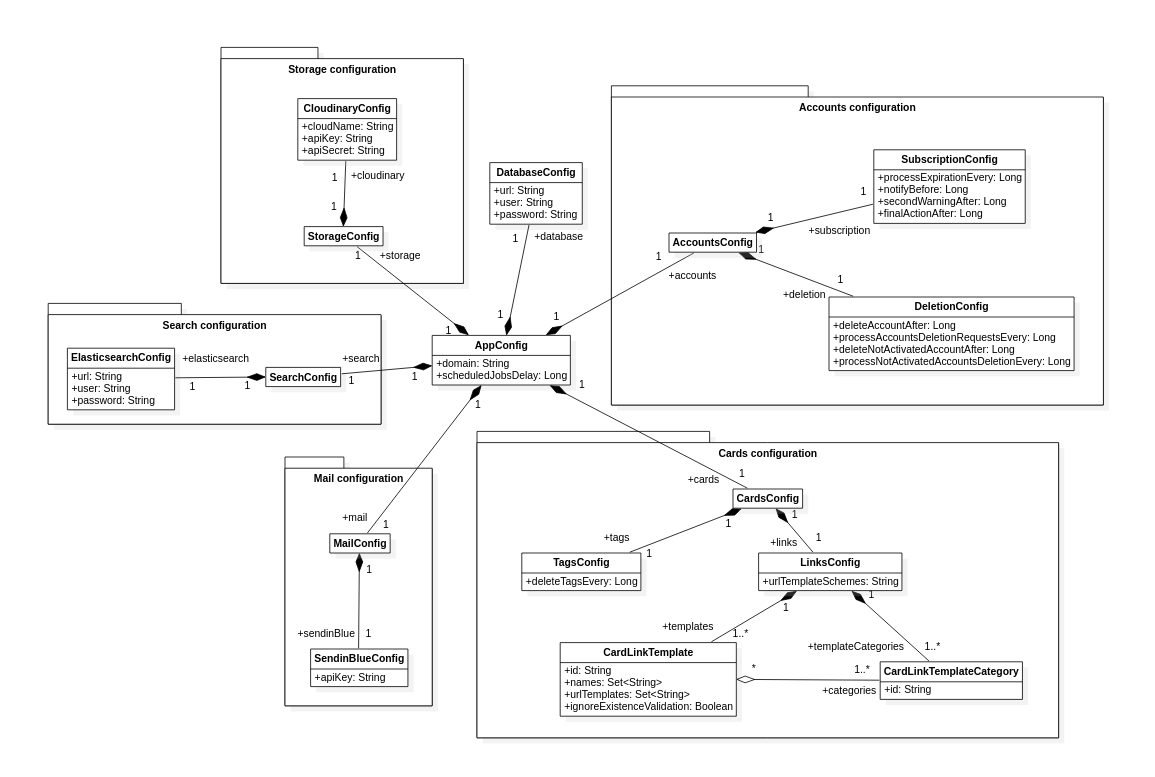
\includegraphics[width=\linewidth]{obrazky/datovy_model_nastaveni_aplikace}\hfill
			\caption{Ukázka datového modelu nastavení aplikace.}
		\end{figure}

		\subsubsection{Šablony odkazů sítí}

		Aby bylo možné uživatelům poskytnou komfort v podobě předdefinovaných sociálních sítí společně s validací \ac{URL} adres,
		bylo potřeba vytvořit robustní systém.
		Byl proto vytvořen systém šablon, kde každá šablona definuje vlastnosti jedné sítě.
		Každý konkrétní odkaz pak má přiřazenou jednu šablonu, na základě které je možné adresu validovat a
		zobrazit uživateli správnou ikonu a název sítě.
		Šablona má tak v první řadě hlavně unikátní identifikátor, oficiální název a ikonu.
		Dále má kolekci možných názvů a zkratek pro potřeby pohodlného vyhledávání.
		Nejdůležítějšími daty pro validaci jsou šablony \ac{URL} adres a příznak zda se má validovat konkrétní \ac{URL} adresa odkazu.

		\begin{lstlisting}[language=Java]
public class CardLinkTemplate {
    String id;
    Set<String> names;
    Set<String> urlTemplates;
    Set<CardLinkTemplateCategory> categories;
    boolean ignoreExistenceValidation;
}
		\end{lstlisting}
		Ukázka možných nastavení pro každou šablonu sítí. % TODO

		% todo
		názvy podle kterých lze šablony vyhledat v uživatelské administraci
		validní URL adresy
		kategorie, ve kterých lze šablonu vyhledat
		zda se má validovat existence odkazu s touto šablonou

			\paragraph{Šablony URL adres}

			Šablony \ac{URL} adres slouží pro specifikování vzoru povolených \ac{URL} adres dané sítě.
			Tím je zaručeno, že odkaz vede skutečně na ověřenou sít a jen se tak netváří.
			Zároveň to umožňuje získat u \ac{URL} adresy ID uživatelského profilu na cílové síti pro možnosti fulltextového
			vyhledávání karet podle těchto identifikátorů.

			S pomocí speciálních vyhrazených sekvencí znaků je tak možné definovat poměrně velké množství kombinací
			šablon.
			Šablony jsou pak následně zanalyzovány a vytvoří se z nich Regex výrazy, pomocí kterých dokáže Java zjistit
			zdá daný textový řetězec odpovídá nějakému výrazu.
			Regex je výrazový jazyk skládající se ze speciálních znaků definující pravidla porvnávání \cite{regex}.
			Systém momentálně podporuje sekvence \lstinline{*} a \lstinline!{userPart}!.
			Sekvence \lstinline{*} říká, že se na tomto místě může nacházet jakýkoliv znak vyjma hostové části \ac{URL}
			adresy, kde se mohou pod touto sekvencí skrývat pouze písmena a pomlčky.
			Sekvence \lstinline!{userPart}! může obsahovat stejné znaky jako \lstinline{*} sekvence, avšak textové
			řetězec označený touto sekvenci v cílové \ac{URL} adresa má speciální význam.
			Nachází se v něm totiž právě zmiňované profilové ID.
			Díky tomuto označení je pak systém schopen určit, kde se profilové ID nachází a vytáhnou jej.

			\begin{lstlisting}
https://*.example.com/{userPart}
https://{userPart}.example.com
			\end{lstlisting}
			Ukázka šablon URL adres. % todo

			Systém navíc obsahuje různé validace aplikované při analyzování šablon, aby se do aplikace nemohli načíst
			nevalidní šablony.
			Momentálně definovanými pravidly URL šablon jsou následující:
			\begin{itemize}
				\item právě jedna sekvence \lstinline{userPart}
				\item oddělovač mezi jednotlivými sekvencemi
				\item šablona je po záměně sekvencí validní URL adresa
			\end{itemize}

			\paragraph{Validace odkazů}

			Na základě nakonfigurovaných šablon URL odkazů je možné konkrétní odkazy validovat.
			Standardní validace se skládá ze dvou hlavních částí.
			První část řeší jestli \ac{URL} adresa odpovídá předpokládané šabloně sítí.
			Předpokládaná šablona je určena nadřazenou skupinou odkazů.
			Validátor se pak pokusí nalést existující šablonu z předané URL adresy.
			Pokud je tento předpoklad splněn a zároveň se má validovat existence adresy, přechází validátor do druhé části.
			Druhá část se zabývá validací existence \ac{URL} adresy, tj. zda URL adresa odkazuje na nějakou existujicí
			webovou stránku.
			Toto se ověřuje simulováním \ac{HTTP} požadavku webového prohlížeče a z odpovědi se zjistí, že buď stránka
			existuje, stránka neexistuje nebo URL adresa přesměrovává na jinou stránku.
			V prvních dvou případech validace končí.
			V tom posledním se proces opakuje s novou vrácenou URL adresou.
			I u této adresy se kontroluje šablona a existence.
			Takto se proces opakuje do té doby než validátor dostane jasnou odpověď existence nebo vyprší interně stanovený
			limit přesměrování.
			Limit byl zaveden, aby nemohlo dojít k potencionálnímu zacyklení validace.
			Je ale nastaven dostatečně vysoký, aby nedocházelo k předčasným selhání validací.

			\begin{figure}[H]
				\centering
				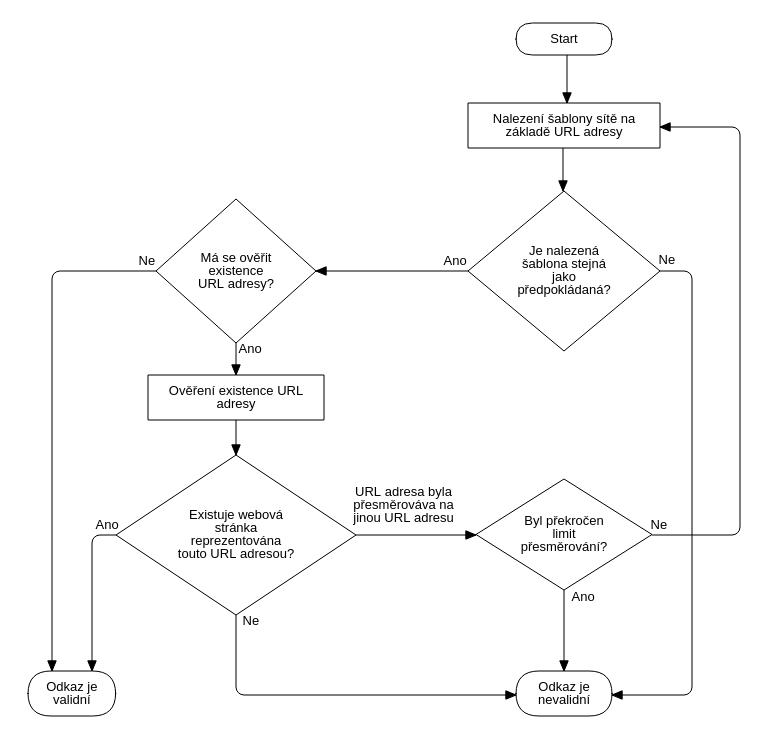
\includegraphics[width=\linewidth]{obrazky/proces_validace_odkazu}\hfill
				\caption{Proces validace URL adresy odkazu. Zdroj: [autor]}
			\end{figure}

			Bohužel ne u všechn URL adres lze validovat existence.
			Některé stránky totiž mají pokročilou ochranu proti škodlivým strojovým botům a tato validace je tedy
			vyhodnocena některými jako škodlými bot.
			Byly provedeny optimalizace v podobě úpravy \ac{HTTP} hlaviček, aby se validace tvářila jako webový prohlížeč
			a u některých stránek to skutečně pomohlo, jiné jsou ale pečlivější.
			Proto se zavedl příznak přímo do definice šablon, který tuto validaci existence vypíná.
			Naštestí se jedná o nižší procenta stránek a pro bezpečnost uživatelů je stěžejní pouze první část validace.

		\subsubsection{Prémiový plán a předplatné}

		Prémiový plán odemyká uživateli prémiové funkce, které jsou běžně uzamknuté.
		S tím souvisí pojem předplatného popisující stav aktuálního plánu uživatele.
		Prémiový plán lze momentálně aktivovat pouze aplikování kupónu, nicméně systém by měl počítat s budoucím rozšíření
		o možnost předplácet si plán na dobu neurčitou.

		Bez aktivovaného prémiového plánu, uživatel může vytvořit maximálně dvě karty a to navíc bez firemní hierarchie.
		Limity se ale můžou s přibývajícími funkcemi v budoucnu měnit a systém by s tím měl počítat.

		Proces aktivace prémiového plánu začíná aktivováním platného kupónu.
		Na základě této aktivace je uživateli přiřazena speciální role a vytvořen nový popisný objekt předplatného
		definující datum expirace.
		Datum expirace je vypočítán z doby platnosti kupónu.
		Každý kupón definuje po jakou dobu bude předplatné aktivní a při aktivace se tato doba přičte k aktuálnímu datumu.
		V tuto chvíli uživatel může využívat všechny prémiové funkce.
		Pokud v tuto chvíli uživatel aplikoval další jiný kupón, datum expirace by změnil podle nového kupónu.

		V případě placeného předplatného by objekt předplatného zprvu neměl datum expiraci.
		Ta by se nastavila automaticky až při neprovedené následující platbě.

		Systém tedy při vytváření a ukládání karet musí vždy validovat zda daná karta neobsahuje prémiový obsah.
		Pokud ano, musí zkontrolovat, zda-li uživatel má příslušnou roli.
		V případě, že by neměl, je celý požadavek zaříznut a uživateli je vrácena chyba.

		Nejkomplikovanější částí celého systému je expirace předplatného.
		Problém spočívá v existenci prémiového obsahuje.
		Pokud uživatel v době expirace nemá prémiový obsah na svém účtu, je situace jednoduchá a předplatné se zruší.
		Pokud však uživatel prémiový obsah na svém účtu má v době expirace, je potřeba definovat způsob jakým se
		s takovými daty naloží.
		Uživatel pak v takovém případě má tři možnosti.
		Tou nejjednodušší je upozornění ignorovat a v takovém případě se po nějaké době všechny karty uživatele skryjí
		a veřejnost je na ně již nepodívá.
		Druhou možností je prémiový obsah pomocí speciálního formuláře odstranit, aby bylo možné zrušit předplatné.
		Poslední možností je prodloužení předplatného.
		V tomto případě uživateli všechen obsah zůstane a může prémiové funkce nadále využívat.

		Celý proces začíná nějakou dobou před samotnou expirací.
		Uživatel je dopředu upozorněn na blížící se expiraci emailem.
		Pokud uživatel do té doby nesmaže všechen prémiový obsah, v den expirace přijde druhý email s informací o
		proběhlé expiraci a možnosti, které uživatel může provést.
		Pokud bude uživatel ignorovat toto upozornění, během několika dnů mu přijde druhé stejné upozornění.
		V případě, že uživatel ignoruje i toto poslední varování, všechna data uživatele jsou během několika dnů
		automaticky skryta.
		Uživateli už jen přijde informativní email o skrytí dat.

		Zvolený přístup se jeví jako dostatečně flexibilní a pokrývající všemožné scénáře požadované aplikací.

		\subsubsection{REST API}

		K zajištění komunikace mezi front-endovou \ac{GUI} aplikací a aplikací \ac{API} serveru, server
		vysvavuje právě \ac{REST} \ac{API}.
		Díky němu je možné vytvářet, ukládat a získávat entity a spouště různé akce.

		\ac{REST} \ac{API} obecně pracuje s tzv. zdroji.
		Každý zdroj představuje jeden typ pojmenovatelné informace.
		Tím může být třeba entita, obrázek, dokument nebo kolekce.
		Jednotlivé zdroje jsou pak vystaveny na přesně daných \ac{URL} adresách a pomocí \ac{HTTP} metod (GET, POST, PUT...)
		je možné s těmito zdroji provádět operace.
		Operacemi jsou většinou následující: získání konkrétního zdroje nebo kolekce, vytvoření nového zdroje na základě
		předaných dat nebo úprava již existující zdroje opět na základě předaných dat.
		Nejrozšířenějším jazykem pro popis zdrojů je \ac{JSON}, díky kterému je možné objekty aplikace poměrně jednoduše
		mapovat na \ac{JSON} dokumenty. \cite{restfulapi}

		Implementované \ac{API} v běžných scénářích (získání, vytvoření, úprava zdrojů) respektuje doporučovaná pravidla.
		Nicméně v krajních případech je potřeba provádět i jiné, většinou servisní, operace, které tyto pravidla porušují.
		Toto je však poměrně běžná praxe, a pokud takto není navržena větší část \ac{API}, tak to většinou nepředstavuje
		problém.

		Jak je možné vidět níže, \ac{API} pro uživatelské účty zahrnuje manipulaci s účtem přihlášeného uživatele a manipulaci
		s oblíbenými kartami.

		\begin{figure}[H]
			\centering
			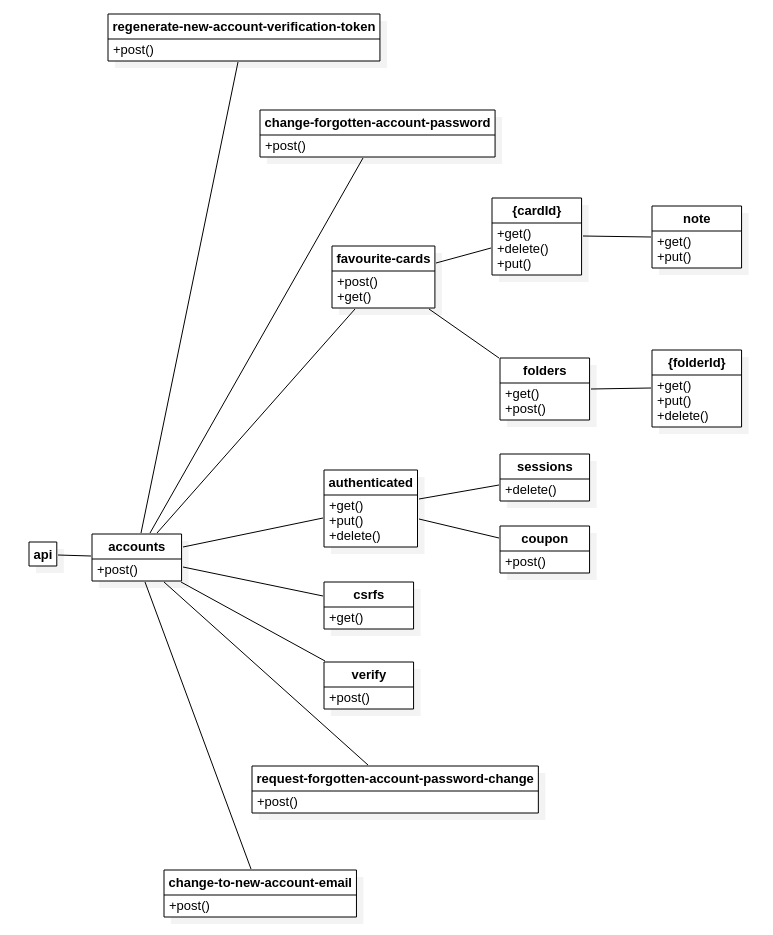
\includegraphics[width=\linewidth]{obrazky/api_model_ucty}\hfill
			\caption{Stromový přehled struktury API uživatelských účtů. Zdroj: [autor]}
		\end{figure}

		Nejpodstatnější \ac{API} se zabývá manipulací karet a zároveň umožňuje získávat i další podržezané entity.
		Mimo to nabízí i pomocné operace pro manipulaci s display ID.

		\begin{figure}[H]
			\centering
			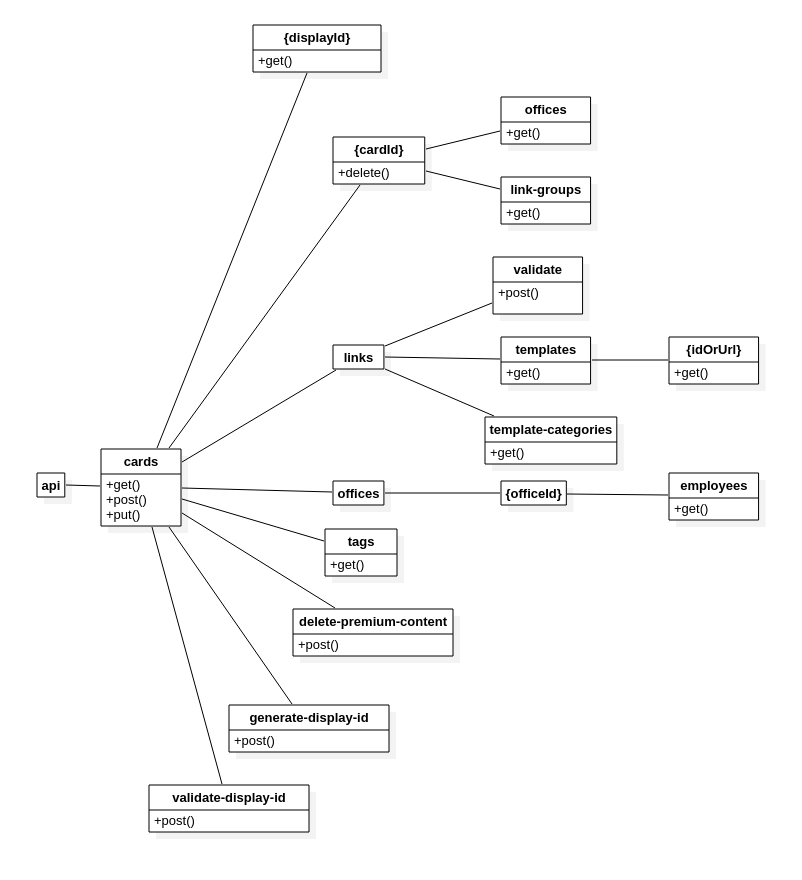
\includegraphics[width=\linewidth]{obrazky/api_model_karty}\hfill
			\caption{Stromový přehled struktury API karet. Zdroj: [autor]}
		\end{figure}

		\ac{API} úložiště momentálně umožňuje pouze soubory nahrávat, protože systém pracuje pouze s věřejnými soubory, které
		lze získat přímo z Cloudinary serverů.

		\begin{figure}[H]
			\centering
			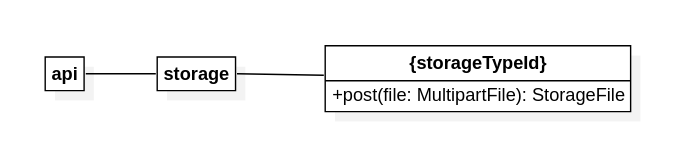
\includegraphics[width=8cm]{obrazky/api_model_uloziste}\hfill
			\caption{Stromový přehled struktury API uložiště. Zdroj: [autor]}
		\end{figure}

		Pro vyhledávání karet a míst existuje separátní vyhledávací \ac{API} pro přehlednost.

		\begin{figure}[H]
			\centering
			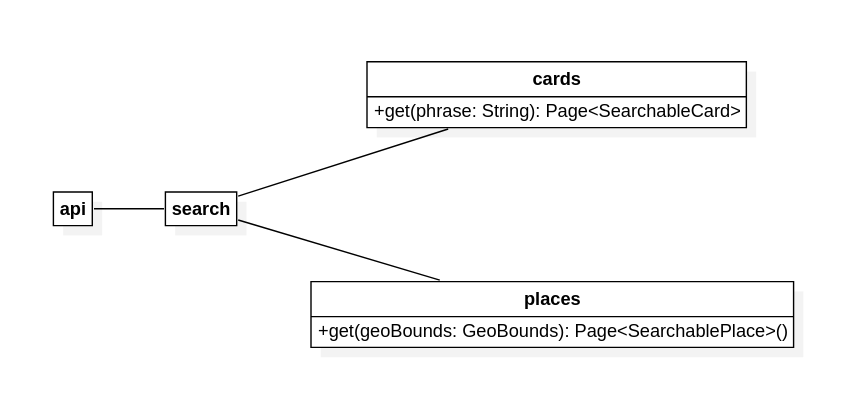
\includegraphics[width=8cm]{obrazky/api_model_vyhledavani}\hfill
			\caption{Stromový přehled struktury API vyhledávání karet. Zdroj: [autor]}
		\end{figure}

		Aplikace také nabízí interní administraci celé aplikaci pro správce.
		Proto vzniklo i \ac{API} pro spouštění servisních operací a k správě zákulisních zdrojů (např.: kupóny).

		\begin{figure}[H]
			\centering
			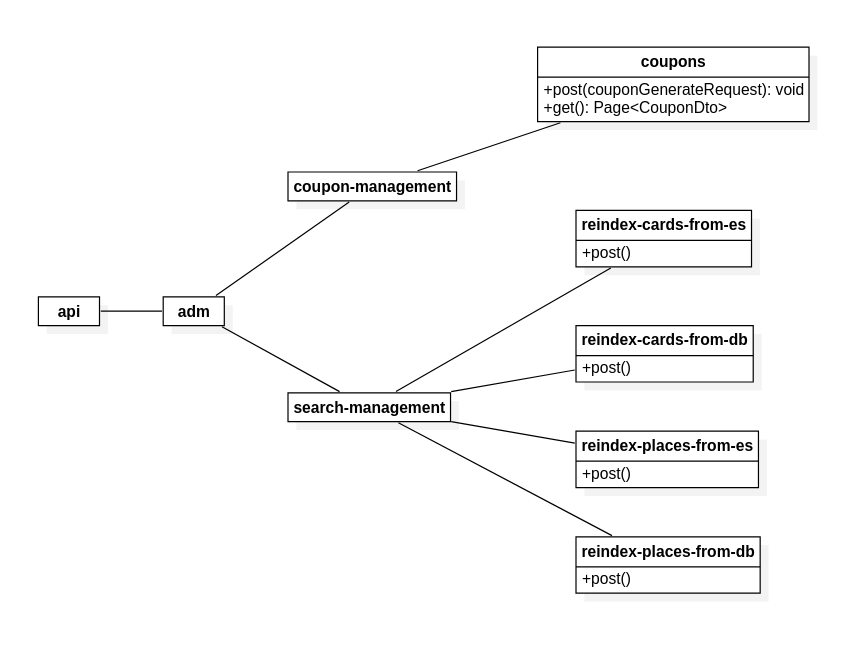
\includegraphics[width=\linewidth]{obrazky/api_model_adm}\hfill
			\caption{Stromový přehled struktury API operací administrace. Zdroj: [autor]}
		\end{figure}

			\paragraph{Objekty pro přenos dat}

			V rámci komunikace mezi konzumentem \ac{API} a serverem je nezbytné přenášet objekty reprezentující data
			aplikace.
			K tomu by šlo přímo využít datových tříd z business logiky.
			Bohužel některé tyto třídy obsahují data, která by se neměla dostat ven ze serveru.
			Nejtypičtějšími takovými daty jsou hesla uživatelů.
			Nicméně někdy je také nezbytné poskytnout agregované atributy, které však nemají své místo v originálních datech.
			Právě z těchto důvodů \ac{API} využívá tzv. objektů pro přenost dat \ac{DTO}.
			Tyto datové objekty slouží obecně pro přenos daty mezi procesy.
			V tomto případě přenáší data mezi \ac{API} serverem a front-endovou aplikací.

			\ac{API} tak na venek pracuje pouze s \ac{DTO} objekty reflektující doménové objekty.
			Speciálním případem jsou \ac{DTO} objekty nemající ekvivalentní doménový objekt a slouží tak pouze pro jednorázové
			předání dat.
			Většinou se používají pro specifikování požadavků front-endové aplikace na zvolenou operace nebo jako
			objekty nesoucí výsledek nějaké operace.

			Pro transformaci mezi doménovými objekty a \ac{DTO} objekty vznikla jednoduchá podpora pro standardizovanou
			a centralizovanou transformaci.
			Slouží k tomu továrnové třídy dědící z obecného rozhraní zpřístupňující metodu pro transformaci z doménového
			objektu na \ac{DTO} objekt a metodu pro obráceno transformaci.

			\begin{lstlisting}[language=Java]
public interface DtoFactory<E, D> {
    D createDto(E entity);
    E updateEntity(E originalEntity, D dto);
}
			\end{lstlisting}
			Ukázka obecného rozhraní třídy pro transformaci mezi doménovými objekty a DTO objekty. % todo

			Transformace z \ac{DTO} objektu na doménový objekty je specifická v tom, že pro transformaci používá zároveň
			i originální doménový objekt z databáze.
			Díky tomu je možné zajistit, že výsledný objekt bude mít změněné pouze ty atributy, které jsou povolené.

			Rozhraní továrny je generické a proto pro každou transformovatelnou entitu je potřeba implementovat konkrétní
			transformaci.
			Každá entita má vlastní doménovou třídu a vlastní \ac{DTO} třídu a především jiná data a jiný způsob transformace.

			\paragraph{Zabezpečení}

			Zabezpečení je velmi důležitou součástí aplikace pro znemožnění zneužití dat útočníky.
			Je nezbytné zajistit, aby se neoprávnění uživatelé nedostali k datům, které jim nepřísluší a aby nemohl
			poškodit cizí data.
			Těmito problémy se zabývá především společnost OWASP poskytující kvalitní materiály o bezpečnosti programátorům.
			Avšak řešit všechny existující problémy svépomoci by zabralo spoustu času a bez dlouholetých znalostí v
			oblasti bezpečnosti, by implementovaný systém nemusel být ani správně zabezpečený.
			Navíc nové hrozby stále vznikají a udržovat bezpečnostní systém paralelně s rozšiřováním aplikace by vyžadovalo
			celý tým vývojářů.

			Naštěstí framework Spring zahrnuje i knihovnu Spring Security pro zabezpečení celé webové aplikace.
			Tato knihovna jednak automaticky zajišťuje doporučené bezpečnostní praktiky a jednak poskytuje programátorovi
			nástroje pro tvorbu přihlašování a práv uživatelů.
			Knihovna obsahuje předpřipravené nástroje pro běžné postupy přihlašování a implementaci práv.
			Programátor si však tyto nástroje může relativně snadno rozšířit nebo implementovat vlastní.

			Specificky pro tuto aplikaci bylo definováno jaké \ac{URL} adresy \ac{API} vyžadují přihlášení a specifické
			role a výchozí přihlašovací proces byl rozšířen o externí poskytovatele a vlastní správu účtů.

			\begin{lstlisting}[language=Java]
@Override
protected void configure(HttpSecurity http) throws Exception {
        http
            .mvcMatchers(HttpMethod.GET, "/api/search/cards").permitAll()
            .mvcMatchers(HttpMethod.GET, "/api/search/places").permitAll()
            .mvcMatchers("/api/adm/**").hasRole("ADMIN")
            .mvcMatchers("/api/**").authenticated()
            .anyRequest().denyAll()
        /* ... */
}
			\end{lstlisting}
			Ukázka části nastavení zabezpečení pomocí knihovny Spring Security. % todo

			% todo
			tuto URL adresu mohou využívat i nepřihlášení uživatelé
			tuto URL adresu mohou využívat i nepřihlášení uživatelé
			URL adresy s tímto vzorem mohou využít jen uživatelé s rolí ADMIN
			všechny ostatní URL adresy začínající "/api" prefixem využadují přihlášeného uživatele
			ostatní URL adresy nemůže využít nikdo

			\paragraph{Přihlašování}

			Korektní implementace procesu přihlašování je pro aplikaci využívající uživatelské účty stěžejní.
			Zabraňuje neoprávněným uživatelům vydávat se za jiné uživatele.
			Standardním, dlouhá léta využívaným, přístupem je ověření kombinace emailové adresy/uživatelského jména
			a hesla.
			U tohoto přístupu kombinaci ověřuje přímo aplikace.
			Druhým, stále více používaným, přístupem je přihlašování pomocí třetích stran.
			Při tomto přístupu aplikace deleguje přihlašování na jiného poskytovatele uživatelských účtu, který následně
			vrátí po přihlášení původní aplikaci informace o přihlášeném uživateli.
			Aplikace se tak nemusí starat o ověřování hesla a podobně.
			Takovýchto poskytovatelů existuje celá řada, což pomohlo vzniknout standardu OAuth2 standardizující proces
			komunikaci mezi aplikací a poskytovatelem.
			Díky tomu není potřeba pro každého poskytovatele implementovat odlišný proces.

			Aby měli uživatelé volnost při výběru, jakým způsobem se chtějí přihlašovat, byly do této aplikace implementovány
			oba způsoby.
			Uživatel se tak může přihlásit a zaregistrovat buď pomocí běžné kombinace emailové adresy a hesla nebo pomocí
			některých z poskytovatelů.
			Momentálně jsou připraveni nejvýužívanější poskytovatelé Google, Github a Facebook, nicméně rozšíření o
			další poskytovatele nepředstavuje příliš práce.
			Zaregistrovaný uživatel si navíc může ke svému účtu připojit i další způsoby, tj. pokud se zaregistroval emailovou
			adresou, může si připojit některého z poskytovatelů a obráceně.
			Díky tomu si uživatel může při každém přihlášení vybrat, jakým způsobem se přihlásí.

			Druhým řešeným problémem je, jak verifikovat přihlášeného uživatele při každém \ac{HTTP} požadavku na server
			aniž by uživatel musel zadávat přihlašovací údaje při každém takovém požadavku.
			Aplikace na serveru může buď udržovat v paměti sezení každého uživatele nebo vygenerovat uživateli token
			obsahující informace o uživateli.

			V případě, že aplikace využívá sezení, je na serveru spravován objekt se informací o přihlášeném uživateli.
			Uživatel pomocí webového prohlížeče pak pouze předává ID daného sezení.
			Server má tak plnou kontrolu nad daným sezením.
			Bohužel server musí opatření proti krádeži těchto ID na úrovni webových prohlížečů

			Alternativou je vygenerování tokenu obsahující uživatelské informace.
			Tento token je následně předán klientovi a ten musí zaručit, aby při každém požadavku předal vygenerovaný token.
			Tento způsob převážně využíván pro komunikaci mezi servery, avšak začíná se používat i v aplikacích, kde
			je aplikace rozdělena na \ac{GUI} část a \ac{API} část.
			Díky tomuto přístupu server nemusí udržovat sezení všech přihlášených uživatelů.
			Tím že ale token nemá pod správou server, není snadné takový token označit jako neplatný v případě odhlášení.
			To jde řešit například ukládáním tokenů do databáze, nicméně správa tokenů se pak částečně přenáší zpět
			na server a výhody nezávislosti na serveru mizí.
			Řešení se tak přibližuje přístupu se sezeními, avšak za cenu sloužitější implementace.

			V případě této aplikace proběhli nějaké experimenty s druhým typem ověřování, posléze se ale ukázalo, že
			řešení je zbytečně složité a ne úplně spolehlivé.
			Přihlašování bylo tedy přepracováno na řešení se sezeními, které Spring Security knihovna má již v základu
			vyřešené na rozdíl od předchozího přístupu.
			Díky tomu se celý proces zjednodušil a delegoval na externí knihovnu, na které pracují experti v oboru.
			Bonusem bylo zjednodušení implementace přihlašování pomocí poskytovatelů třetích stran, protože
			knihovna Spring Security má připravenou podporu pro tyto scénáře.

			Jediným problémem bylo spojení interních uživatelských účtů a OAuth2 účtů.
			Spring Security totiž pro každý způsob využívá jiné objekty.
			Proto byl proces připravený knihovnou rozšířen o vlastní zakončení.
			Toto zakončení je vyvoláno knihovnou po úspěšném přihlášení a dává možnost provést vlastní operace nad
			přihlášeným uživatelem než se odpověď dostane ke koncovému uživateli.
			Proces řeší i registraci nového uživatele, protože OAuth2 nerozlišuje mezi novým a existujícím uživatelem.
			OAuth2 zajišťuje pouze poskytnutí dat o uživatelích.

			Následující diagram popisuje zpracování nově přihlášeného OAuth2 uživatele.

			\begin{figure}[H]
				\centering
				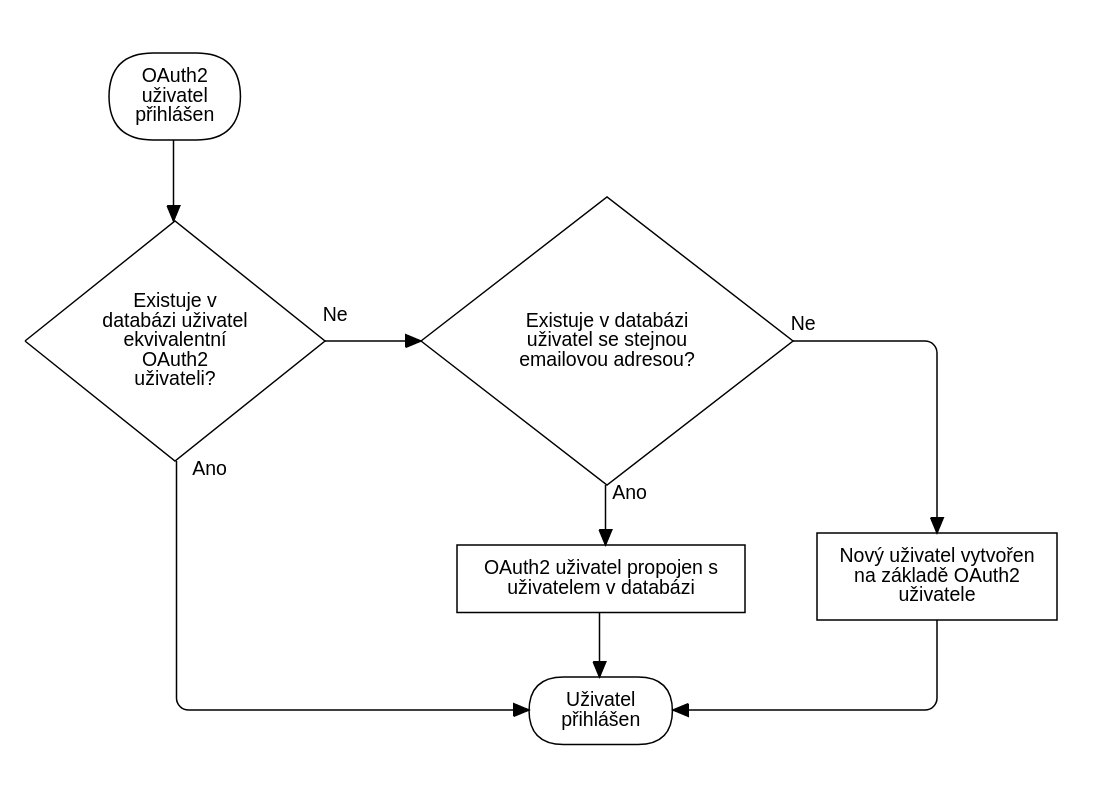
\includegraphics[width=\linewidth]{obrazky/proces_prihlaseni_oauth2}\hfill
				\caption{Proces zpracování přihlášeného OAuth2 uživatele a transformace na interního uživatele. Zdroj: [autor]}
			\end{figure}

		\subsubsection{Automatizované testování}

		Automatizované testování umožňuje kód aplikace otestovat ještě před samotným spuštěním a testovat
		kód průběžně při úpravách a rozšiřováních.
		Díky tomuto testování je možné předejít velkému množství logických chyb již v počátku implementace.

		Způsobů testování je více.
		Tato aplikace využívá tzv. "unit" testování a integrační testování.
		Unit testování izolovaně ověřuje předpokládané chování komponent systému bez ovlivnění chováním
		ostatních komponent\cite{unit_testing}.
		Opakem je integrační testování ověřující souhru více komponent najednou \cite{integration_testing}.

		Služební třídy a pomocné třídy provádějící nějaké transformace (\ac{DTO} továrny, analyzátor šablon odkazů...)
		jsou testovány izolovaně pomocí unit testů.
		Pro každou metodu každé třídy je připraveno několik testů ověřující různé scénáře: běžné chování při různých datech,
		chování při chybných datech a podobně.
		Hlavní knihovnou zpřístupňující nástroje pro spouštění testů a ověřování výsledků je JUnit.
		Aby bylo možné třídy testovat izolovaně, je potřeba simulovat chování ostatních komponent, se kterými testovaná
		třída komunikuje.
		K tomu je využita knihovna Mockito, která zároveň umožňuje zkoumat proběhlé interakce a vyhodnocovat testy
		na základě toho.

		\begin{lstlisting}[language=Java]
@Test
public void getMostUsedTags_ExpectedFoundCorrectOnes() {
	when(cardTagDaoMock.findMostUsed(3)).thenReturn(Set.of(
			new CardTag(null, "dev"),
			new CardTag(null, "nature"),
			new CardTag(null, "tech")
	));
	assertEquals(
			Set.of("dev", "nature", "tech"),
			cardTagService.getMostUsedTags(3)
	);
}
		\end{lstlisting}
		Ukázka Unit testu ověřující, že služba štítků vrací správné nejvyužívanější štítky. % todo

		% todo
		příprava simulace chování repozitáře poskytující data štítků pomocí Mockito knihovny
		ověření, že služba vrací očekávané štítky pomocí JUnit knihovny

		Třídy repozitářů a třídy poskytující \ac{REST} \ac{API} jsou spíše integračními testy spojující více
		komponent k zajištění vypovídajících výsledků.

		Při testování repozitářů je potřeba testovat \ac{SQL} dotazy oproti reálné databázi s daty.
		K spuštění takových testů je tedy potřeba běžící testovací databáze a připravená testovací data.
		Ta jsou do databáze nahrána před každým testem a smazána po každém testu.
		Tím je zaručena izolovanost jednotlivých testů, aby nedocházelo k mylným výsledkům.

		\begin{lstlisting}[language=Java]
@After
public void clean() {
	DbTestUtils.resetTables(
			dataSource,
			CardOffice.TABLE_NAME,
			EmployeeCardData.TABLE_NAME,
			Card.TABLE_NAME,
			Account.TABLE_NAME
	);
}

@Test
@Sql(scripts = "/tests/dao/card/insertMockCards.sql")
public void findById_WithoutDeletedAndNoCard_ExpectedEmpty() {
	assertTrue(cardDao.findById(4, false).isEmpty());
}
		\end{lstlisting}
		Ukázka integračních testů repozitáře karet. % todo

		% todo
		vymaže všechna data z testovací databáze po každém testu
		test ověřující získaní karty z databáze
		nahraje testovací data před spuštěním testu

		Testy \ac{REST} \ac{API} jsou kombinací integračních a unit testů.
		Knihovna Spring poskytuje nástroje pro volání \ac{API} skrze \ac{URL} adresy simulující tak reálnou komunikaci
		s \ac{API}.
		Napojení na služební třídy už je řešeno simulací služebních tříd, aby nebylo nutné zprovozňovat všechny části
		aplikace.

		\begin{lstlisting}[language=Java]
@Test
@WithMockUser
public void validateLink_InvalidLink_ExpectedFalse() {
	/* ... */
	mockMvc.perform(post("/api/cards/links/validate")
					.accept(MediaType.APPLICATION_JSON)
					.contentType(MediaType.APPLICATION_JSON)
					.content(objectMapper.writeValueAsString(requestBody))
					.with(csrf()))
			.andDo(print())
			.andExpect(status().isOk())
			.andExpect(content().contentType(MediaType.APPLICATION_JSON))
			.andExpect(content().json(objectMapper.writeValueAsString(expectedResponseBody)));
}
		\end{lstlisting}
		Ukázka testu volání API validující odkaz. % todo

	\subsection{Implementace front-endové aplikace}

	Front-endová aplikace zpřístupňující \ac{GUI} koncovým uživatelům pro \ac{REST} \ac{API} byla postavena na frameworku
	Nuxt obalující knihovnu Vue.
	Díky tomu je zajištěna reaktivnost komponent a prvotní vykreslení stránek na serveru.
	Zaměření tak padlo na konkrétní problémy řešené domény.

		\subsubsection{Komunikace s API serverem}

		Prvním stavebním kamenem je možnost komunikovat s vyvinutým \ac{API}.
		Opět existuje spousta ověřených knihoven řešící pohodlnou komunikace.
		Nuxt přichází se svou vlastní, která má jednoduché \ac{API} a byla tedy zvolena ta.
		Díky integraci s Nuxt frameworkem bylo možné jednoduše centralizovaně přednastavit knihovnu pro všechna volání \ac{API}.
		Hlavní takovou konfigurací byla správa chyb z volání \ac{API}.
		Ta řeší obecné chyby jako nepřihlášený uživatel nebo nedostačená práva uživatele.
		Zároveň řeší aby v každém požadavku byl zahrnut platný \noindent\ac{CSRF} token.
		\ac{CSRF} token zabraňuje útočníkům provádět operace pod účet jiného uživatele pomocí podvodných stránek \cite{csrf}.
		Token je poskytován \ac{API} serverem na vyžádání.
		Front-endová aplikace však musí zaručit jeho získání a následné uložení pro další požadavky.
		To je zajištěno přidáním \ac{CSRF} tokenu do speciální hlavičky \ac{HTTP} požadavku ještě před odesláním požadavku.
		Pokud token v aplikaci ještě neexistuje, je odeslán paralelní požadavek na \ac{API} server pro vygenerování tokenu.

		\begin{lstlisting}
$http.onRequest(async (request) => {
	if (!csrfAllowedMethods.includes(request.method)) {
		await addCsrfTokenToRequest(store, $http, request)
	}
})
		\end{lstlisting}
		Ukázka vložení CSRF tokenu do každého požadavku putujícího na API server. % todo

		\subsubsection{Centrální zdroj informací}

		Dalším důležitým stavebním prvkem je tzv. centrální zdroj informací.
		Ten představuje centralizované místo pro ukládání a získávání dočasných dat napříč celou aplikací.
		Je zde možné například uložit informace o přihlášeném uživateli nebo výše zmíněný \ac{CSRF} token.
		K tomu slouží knihovna Vuex řešící uchování dat a záznam změn dat v čase.
		Díky ní je pak uživatelský účet jednoduše přístupný ze všech komponent bez nutnosti opakovaného provolávání
		\ac{API} serveru.

		\subsubsection{Lokalizace textů}

		Lokalizace textů se zabývá zobrazováním textů prvků \ac{UI} v konkrétním jazyce uživatele.
		Díky tomu různí uživatelé mluvící odlišnými jazyky mohou bez problému aplikaci využívat jejich nativním jazyce.
		Tuto problematiku je dobré řešit hned na počátku implementace potencionálně vícejazykové aplikace.

		Knihovna i18n of tvůrců frameworku Nuxt tuto problematiku řeší.
		Konkrétně zajišťuje nahrazování klíčů konkrétními texty v komponentech a automatické přepínání použitého jazyka
		podle webové prohlížeče.

		\begin{lstlisting}
{
  "general": {
    "button": {
      "add": "Add",
      "apply": "Apply",
  /* ... */
}
		\end{lstlisting}
		Ukázka souboru s mapováním klíčů na texty pro anglický jazyk. % todo

		\begin{lstlisting}[language=HTML]
<button>
	{{ $t('general.button.apply') }}
</button
		\end{lstlisting}
		Ukázka definování klíče na stránce, který je při vykreslení stránky nahrazen textem. % todo

		Problém ale nastal při tvorbě informačních stránek (nápověda, podmínky použítí...).
		U těchto stránek je obsah zapsán jako jeden velký \ac{HTML} soubor pro podporu formátování, nikoliv
		jako dílčí texty.
		Knihovna totiž očekává všechny texty zapsané v jednom \ac{JSON} dokumentu.
		Do těchto dokumentů tedy bylo potřeba nějakým způsobem vložit i ty \ac{HTML} dokumenty.
		Z tohoto důvodu pro každý jazyk vznikl \ac{JS} soubor, který posbírá všechny překladové materiály a poskládá z nich
		výsledný \ac{JSON} dokument se všemi překladovými texty.

		\begin{lstlisting}
import cardLinkTemplates from '../universal/card-link-templates.json'

import lang from './en/en.json'

import helpAboutContent from './en/help/about-content.help'
import helpCookiesContent from './en/help/cookies-content.help'
import helpPrivacyContent from './en/help/privacy-content.help'
import helpTermsContent from './en/help/terms-content.help'
import helpSupportBasicContent from './en/help/support-basic-content.help'
import helpSupportSecurityContent from './en/help/support-security-content.help'

lang.card.link.template = cardLinkTemplates
lang.help.about.content = helpAboutContent
lang.help.cookies.content = helpCookiesContent
lang.help.privacy.content = helpPrivacyContent
lang.help.terms.content = helpTermsContent
lang.help.support.basic.content = helpSupportBasicContent
lang.help.support.security.content = helpSupportSecurityContent

export default lang
		\end{lstlisting}
		Ukázka sestavení JSON dokumentu se všemi překladovými texty. % todo

		\subsubsection{Validace formulářových polí}

		Validace uživatelsky vložených dat je důležitá především pro zaručení správnosti uložených dat.
		Ne všichni uživatelé jsou však podvodníci chtějící poškodit data.
		Většina uživatelů zadávají očekávaná data, nicméně je velká pravděpodobnost, že se nějaký uživatel omylem upíše
		a udělá nechtěnou chybu.
		Proto je dobré v rámci kvalitního \ac{UX} poskytnou uživatelům rychlou a cílenou zpětnou vazbu o chybně zadaných
		datech.

		\begin{figure}[H]
			\centering
			
\includegraphics[width=8cm]{obrazky/nevalidni_pole_formulare}\hfill
			\caption{Ukázka pole formuláře s textem v nevalidním formátu. Zdroj: [autor]}
		\end{figure}

		Pomocí knihovny Vuelidate bylo možné snadno implementovat zobrazování chyb přímo v konkrétních polích
		hned jakmile uživatel vyplní dané pole.
		Knihovna řeší celý mechanismus validace hodnot polí a poskytování výpisu všech chyb ve formuláři.
		Zároveň přichází s obecnými validátory, ale programátor může implementovat vlastní.
		Toho bylo využito například u validace \ac{URL} adresy odkazu na sociální síť, kdy je potřeba se dotázat \ac{API},
		které adresu zvaliduje.

		\begin{lstlisting}
export const displayId = function (cardId) {
	return async function (displayId) {
		const requestBody = { cardId, displayId }
		try {
	  		return (await this.$http.$post('cards/validate-display-id', requestBody)).valid
		} catch (e) {
		    this.$notifyError()
		}
	}
}
		\end{lstlisting}
		Ukázka implementace vlastního validátoru využívající API k validaci hodnoty. % todo

		S připravenými dílčími validátory je pak možné definovat pravidla pro jednotlivá pole ve formuláři.
		Tyto pravidla jsou následně aplikována na jednotlivá pole, která sledují změnu hodnoty a informují o tom změnách
		a případných chybách formulář.
		Díky reaktivnosti Vue je pak možné chybu zobrazit hned jakmile vznikne.
		Následně při odeslání formuláře uživatelem, je validace provedena ještě jednou a buď je formulář odeslán nebo
		zobrazena chyba.
		V případě běžných uživatelů by se tedy na server vůbec chybná data neměla dostat.

		\begin{lstlisting}
validations () {
	return {
		card: {
			name: {
				required,
				minLength: minLength(3)
			},
			displayId: {
				required,
				minLength: minLength(2),
				maxLength: maxLength(64),
				displayIdFormat,
				displayId: displayId(this.card.id)
			}
		}
	}
}

submitForm () {
	this.$v.$touch()
	if (!this.$v.$invalid) {
		/* ... */
	}
}
		\end{lstlisting}
		Ukázka definice pravidel polí a odeslání formuláře. % todo

		% todo
		definice pravidel polí
		poslední validace a odeslání formuláře
		naposled zvalidovat data ve formuláři, pokud budou nevalidní, chyby se zrovna zobrazí

		\subsubsection{Upozornění v UI}

		Pokud v aplikace vznikne nějaká událost o které by měl být uživatel okamžitě informován (chyba, úspěšnost operace...).
		To je v tomto případě vyřešeno vyskakujícími upozorněnými po vzoru upozorněních využitých v mobilních operačních
		systémech.
		Tento způsob je výhodný v tom, že uživatel si upozornění všimne ať už je kdekoliv na stránce.
		Zároveň při přechodu mezi modálními okny se upozornění neztratí.

		\begin{figure}[H]
			\centering
			
\includegraphics[width=6cm]{obrazky/upozorneni_chyba}\hfill
			\caption{Ukázka upozornění na chybu vzniklou špatnými přihlašovacími údaji. Zdroj: [autor]}
		\end{figure}

		K implementaci upozornění byla využita knihovna \url{https://www.npmjs.com/package/vue-notification}{Vue.js notifications}
		poskytující dostatečnou volnost přizpůsobení vzhledu a chování oproti ostatním podobným knihovnám.
		Je navíc na míru tvořena pro knihovnou Vue.
		Knihovna poskytuje jednoduché \ac{API} pro vystavování upozornění pomocí specifikování typ zprávy (chyba, úspěch, info...)
		samotné zprávy.
		Pro velkou aplikaci, kde je nutné na spoustě místech taková upozornění vystavovat je nevhodné duplikovat
		pokaždé celou specifikaci upozornění.
		Stejně jako komponenty i upozornění využívají překladových textů.
		Tato kombinace tak značně zvyšuje riziko chybovosti délky kódu.
		Vznikla proto jednoduchá abstrakce zpřístupňující pomocné metody dostupné skrze celou aplikaci.
		Pro každý používaný typ zprávy (chyba, úspěch, info) existuje právě jedna metoda vyžadující pouze klíč překladového textu.
		Malou výjimkou jsou chybové zprávy, kde existují dvě metody: jedna s možností vložení vlastního textu, druhá
		zobrazující generickou chybu.

		\begin{lstlisting}
this.$notifySuccess('general.success.added')
this.$notifyInfo('general.info.linkCopied')
this.$notifyError('general.error.invalidData')
this.$notifyError()
		\end{lstlisting}
		Implementované pomocné metody pro vystavení různých typů upozornění. % todo

	\subsection{Příprava pro produkční provoz}

	Tím že celá aplikace poběží na orchestračním systému Kubernetes, je nutné zprovoznit obě aplikace v Docker kontejnerech.
	Následně nakonfigurovat Kubernetes, aby sám aplikace spustil a navázal mezi nimi spojení.

		\subsubsection{Příprava Docker image}

		Docker image je šablona, podle které se automatizovaně vytvářejí běžící kontejnery obsahující běžící aplikace.
		Pro \ac{API} server aplikaci a front-endovou aplikaci je nutné tedy připravit separátní Docker image.
		K tomu poslouží speciální soubor zvaný Dockerfile sloužící jako předloha pro vytvoření Docker image.
		Dockerfile obsahuje všechny příkazy potřebné pro spuštění aplikace \cite{dockerfile_reference}.

		Součástí nadstavby Spring frameworku Spring Boot je možné automatizovaně Docker image vytvořit bez manuální tvorby
		Dockerfilu.
		Tato funkcionalita vychází ze standardizované struktury aplikací postavené na Spring Boot knihovně.
		Díky ní je Spring Boot schopen automatizovaně vytvořit optimalizovaný Docker image celé aplikace připravené k
		použití.
		Tato aplikace naštěstí nevybočuje ze standardizované struktury Spring Boot aplikací, a proto byla tato podpora využita.

		V případě front-endové aplikace tato podpora není a bylo nutné Dockerfile připravit ručně.
		Nicméně příprava front-endové aplikace pro provoz v Docker kontejneru byla jednodušší než by byla příprava \ac{API}
		serverové aplikace.
		Dockerfile obsahuje příkazy podobné tomu jak se aplikace spouští pro lokální vývoj.
		Dockerfile nejdříve vytvoří cílový adresář pro aplikace a nainstaluje potřebné systémové aplikace pro sestavení
		a běh aplikace.
		Následně aplikaci sestaví do vytvořeného adresáře a aplikaci spustí na portu \lstinline{3000}.

		\begin{lstlisting}
FROM node:14.17.6-alpine

RUN mkdir -p /usr/src/netreachme-web-app
WORKDIR /usr/src/netreachme-web-app

RUN apk update && apk upgrade
RUN apk add git

COPY . /usr/src/netreachme-web-app/
RUN npm install yarn
RUN yarn install
RUN yarn build

EXPOSE 3000

ENV NUXT_HOST=0.0.0.0
ENV NUXT_PORT=3000

ENTRYPOINT yarn start --dotenv=.env.$ENV
		\end{lstlisting}

		\subsubsection{Nastavení Kubernetes}

		S připravenými Docker imagi pro obě aplikace bylo možné zprovoznit Kubernetes systém.
		V systému běží především implementované aplikace.
		Společně s nimi se zde nachází i webový server nginx a databázový systém Elasticsearch.
		Jediný primarní databáze PostgreSQL je provozována samostatně poskytovatelem DigitalOcean.
		Není tak nutné se starat o ruční zálohovaní a výpadky.

		\begin{figure}[H]
			\centering
			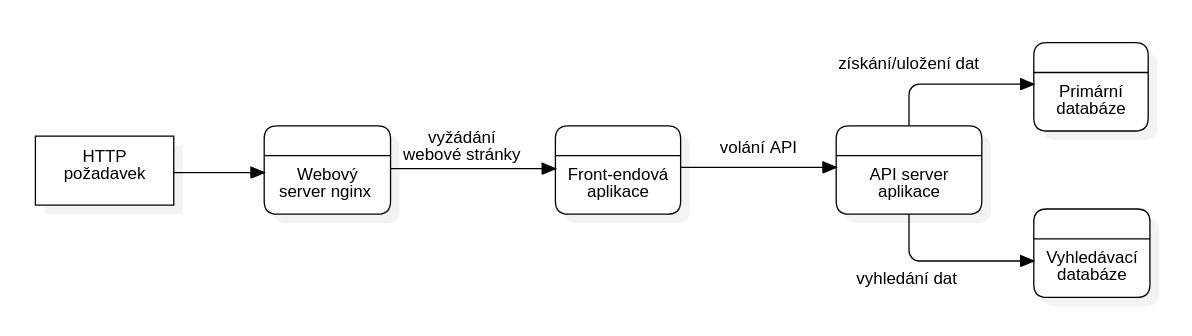
\includegraphics[width=\linewidth]{obrazky/architektura_produkce}\hfill
			\caption{Ukázka putování HTTP požadavku infrastrukturou. Zdroj: [autor]}
		\end{figure}

		Webový server slouží jako vstupní brána do celého systému a poskytuje nástroje pro zabazpěčení
		zpracování požadavků.
		Zároveň zahazuje neplatné požadavky ještě dřív než by mohli způsobit škody v samotných aplikacích.
		Ten následně platné požadavky deleguje na serverovou část front-endové aplikace s požadavek na poskytnutí aplikace.
		V případě, že jsou vyžadována data z API server, front-endová aplikace část požadavku deleguje právě na \ac{API}.
		\ac{API} server si data může navíc vyžádata z primární databáze nebo vyhledávácí databáze.
		Zpracovaný požadavek se nakonec vrací uživateli opět skrze nginx.

		Obě aplikace a server nginx jsou nakonfigurované jako Deploymenty a Elasticsearch jako StatefulSet.
		Deployment je entita Kubernetes systému popisující jak bude aplikace spuštěna \cite{deployements}.
		Deploymenty se používají v případě kdy aplikace neudržuje důležitá data, o která by se v případě vypnutí přišlo
		\cite{deployements}.
		StatefulSety jsou jakousi nadstavbou nad Deploymenty a zaručují uržení stavů spuštěných aplikací. \cite{statefulsets}.
		Právě z těchto důvodů mohou být implementované aplikace spouštěné jednodušími Deploymenty, protože všechna důležitá
		data se nachází v databázi PostgreSQL.
		Elasticsearch databáze je na proti tomu sama zdrojem dat a není vhodné, aby docházelo k její vypínání.

		\begin{lstlisting}
apiVersion: apps/v1
kind: Deployment
spec:
	replicas: 1
	template:
		metadata:
			labels:
				app: web-app
		spec:
			containers:
			- image: cloud.canister.io:5000/quickcards/quickcard-web-app:1.0.0
				name: web-app
				env:
					- name: ENV
				value: prod
				ports:
					- containerPort: 3000
		\end{lstlisting}
		Ukázka konfigurace Kubernetes pro spuštění front-endové aplikace. % todo

		O finální spuštění takto nakonfigurovaného Kubernetes systému a vytvoření SSL certifikátů pro bezpečnou komunikaci
		se už postará poskytovatel Kubernetes serveru; v tomto případě DigitalOcean.
		V tomto momentě jsou obě aplikace spuštěny a připraveny zpracovávat uživatelské požadavky.

% ####################################
\section{Závěr}

Tato bakalářské práce se zabývala vývojem webové aplikace pro tvorbu, správu, zobrazení a sdílení vstupních stránek
různých subjektů a objektů.
Vývoj začal návrhem funkčních požadavků definující, které možnosti bude aplikace uživatelům poskytovat.
Mezi hlavní patří tvorba veřejně dostupných vstupních stránek s kontaktními údaji, firemní hierarchií nebo geolokací,
fulltextové vyhledávání a ukládání oblíbených stránek.

Následovala analýza a provonání webových technologií a nástrojů vhodných pro samotnou implementaci.
Výběr obsahoval programovací jazyky a frameworky pro vývoj uživatelského rozhraní a serverové aplikace, nástroje pro návrh
rozhraní a podpůrné systémy.
Mezi technologiemi pro implementaci uživatelského rozhraní se objevily frameworky Vue, React, Angular nebo Swelte.
Z těchto byl vybrán framework Vue pro jeho jednoduchost a kvalitní dokumentaci pro začátečníky.
U jazyků a frameworků pro vývoj serverové části obsahující veškerou logiku aplikace bylo rozhodování mezi Javou,
C\#, PHP a Javascriptem.
Kvůli velmi podobným výhodám napříč programovacími jazyky, byl vybrán jazyk Java společně s frameworkem Spring spíše podle
osobních preferencích a předchozích znalostí.

Další rozhodování se zabývalo výběrem vhodné primární databáze pro uchování uživatelských dat a nástrojem pro
poskytnutí fulltextového vyhledávání.
Výběr zahrnoval populární databáze PostgreSQL, MySQL, Oracle DB, MariaDB a MongoDB.
Na základě požadavků aplikace se výběr zúžil pouze \ac{SQL} databáze z nichž byla vybrána PostgreSQL podle preferencí.
Kromě primární databáze bylo nutné zvolit ještě separátní systém pro fulltextového vyhledávání.
V tomto případě byl vybrán Elasticsearch pro jeho rozšířenost, univerzálnost a možnost lokálního provozu.

Po zvolení všech potřebných technologií, byl v první řadě vytvořen návrh uživatelského rozhraní.
Na zakladě toho byl navržen datový model a zvolen návrhový vzor \ac{DDD} pro strukturování
kódu aplikace.
Na základě modelu byl následně implementován \ac{API} server s veškerou business logikou.
S připraveným funkčním \ac{API} se zaměření přesunulo tvorbu front-endové části podle návrhu uživateslkého rozhraní
komunikující s \ac{API} serverem.

Všechny definované požadavky na aplikaci byly ve výsledku splněny a aplikace byla otestována na produkčním prostředí.
Aplikace je dále otevřena k potencionálním budoucím rozšířením možností pro koncové uživatele.

% todo
% - změnit vzhled FE
% - vymazat todočka z projektů
% - vymazat WIP todočka (hlavně z HP)
% - smazat emaily
% - smazat hesla
% - možná omezit sítě jen na ty co mají nějaké zvláštnosti
% - zajištění přístupu ke službám třetích stran?
% - smazat statistiky
% - připravit český návod pro rozjetí lokálně všeho komplet, asi i s hosts a tak
% - popisky i ke blokům kodu
% - autoři obrátků a kodu i když to je autor
% - vygenerovat poslední stránku https://ris2.uhk.cz/eVSKP/
% - testovací dataset - sql dump
% - žádné zkratky v názvech kapitol
% - mention spriung boot
%GIT21Q4HUB100-7e075147